\newcommand{\ClassPath}{../../../yukibook.cls}
\documentclass{\ClassPath/yukibook}


\begin{document}

    \yukibook{Sistemas Informáticos} % Title
    {Rubén Gómez}  % Author
    {2022-2023}    % Year
    {Técnico superior en \linebreak Desarrollo de  Aplicaciones Multiplataforma} % Name of degree
    {}% catch phrase
    {}% the phrase's author
    {img/portada.png} %cover
    {28436c}
    {si} %mini-title

    \coverpage
%    \licensepage

    \tableofcontents

    %--------------------------------------------------------------------------
    % Start your parts, chapters and sections here
    %--------------------------------------------------------------------------

    \part{Sistemas de numeración y unidades}
    \graphicspath{{../../../temas_comunes/sistemas_de_numeracion/img}}
    \chapter{Sistemas de numeración}
La información que queremos utilizar en un sistema informático debe estar representada de alguna manera que el ordenador pueda entender.

En sistemas orales, o escritos, lo habitual es hacer uso de un idioma concreto mediante un alfabeto conocido. En informática se hace uso de distintos sistemas de numeración para representar tanto números como el resto de información.

\section{Sistema decimal}
El ser humano, desde hace tiempo ha utilizado como sistema para contar el sistema decimal, representado mediante el sistema \href{https://es.wikipedia.org/wiki/N%C3%BAmeros_ar%C3%A1bigos}{arábigo}. Posiblemente se adoptó este sistema por contar con 10 dedos en las manos.

El sistema numérico decimal está basado en diez símbolos ordenados (0, 1, 2, 3, 4, 5, 6, 7, 8, 9), situados de manera ponderada (cada posición tiene un peso específico), que permiten representar las cantidades deseadas. Debido a que hacemos uso de diez símbolos se dice que utiliza la \textbf{base 10}.

%\subsection*{Representación}
Cuando se combina con otros sistemas de numeración, debemos indicar la base en la forma $ \mathbf{19_{(10}} $ , es decir, poniendo un pequeño “\textbf{(10}” a la derecha del número representado la base 10.

La representación de cualquier combinación del sistema decimal se puede representar en forma de potencia, donde la base es 10 y el exponente es la posición en la que se sitúa el símbolo.

Vamos a tomar como ejemplo el siguiente número: \textbf{146}. La representación en forma de potencias:

\begin{center}
    \vspace{-10pt}
    $ 146 = 100+40+6 $

    $ 146 = 1\times100 + 4\times10 + 6\times1 $

    $ 146 =1\times10^2 + 4\times10^1 + 6\times10^0 $
\end{center}

Como se puede comprobar, lo que hemos hecho ha sido coger cada símbolo representado y lo hemos multiplicado por la base (en este caso base 10) y a la base le hemos puesto el exponente de la posición en la que se encuentra. \textbf{El símbolo de más a la derecha tiene como exponente el cero}, y hacia la izquierda el exponente se incrementa en uno para cada posición.


\hypertarget{binario}{}
\section{Sistema binario}

En informática el sistema binario es el más importante ya que es el sistema que internamente utilizan los circuitos digitales. En este sistema sólo se hace uso de dos símbolos, el “0” y el “1”, y por tanto \textbf{su base es 2}. Los dos dígitos se denominan \textbf{bits} (contracción de \textbf{binary digit}).

%\subsection*{Representación}

Para representar que estamos haciendo uso del sistema binario debemos indicar la base al lado del número, por ejemplo: $\mathbf{ 101001_{(2}} $. Como se puede ver es añadir “\textbf{(2}” en pequeño al final del último símbolo.


\section{Sistema hexadecimal}

Esta vez necesitamos dieciséis símbolos ordenados, así que es un sistema de \textbf{base 16}. Para la representación se hace uso de los símbolos numéricos que conocemos (0, 1, 2, 3, 4, 5, 6, 7, 8, 9) y para representar los siguientes, las letras “A”, “B”, “C”, “D”, “E” y “F”, de esta manera formamos los 16 símbolos que necesitamos.

Teniendo en cuenta esto, podemos hacer la representación directa de que $\mathbf{A_{(16} = 10_{(10}}$ y que $\mathbf{E_{(16} = 14_{(10}}$.

En informática es muy habitual hacer uso del sistema hexadecimal a la hora de trabajar con \textbf{bytes} (que es una “palabra” de \textbf{8 bits}). Un símbolo hexadecimal se representa como 4 bits, por lo que necesitaríamos 2 símbolos hexadecimales para un byte.

También se usa durante la edición de código en formato de datos, o durante la programación en ensamblador.

%\subsection*{Representación}
Al igual que con los sistemas anteriores, debemos añadir la base cuando estemos utilizando el sistema hexadecimal: $\mathbf{ F17A_{(16}} $ , $\mathbf{ FBE1D_{(16}} $ , $\mathbf{ 1FAB27_{(16}} $


\section{Sistema octal}
En ordenadores antiguos era habitual hacer uso del sistema octal. Hoy día se usa más como sistema intermedio entre binario y hexadecimal.

Esta vez nos basamos en ocho símbolos ordenados (0, 1, 2, 3, 4, 5, 6, 7), que, al combinarlos, permiten representar las cantidades deseadas. Debido a que hacemos uso de ocho símbolos se dice que utiliza la \textbf{base 8}.

%\subsection*{Representación}
Para representar la base, debemos añadir “(8” a la derecha del número que hayamos indicado, como por ejemplo: $\mathbf{ 770_{(8} }$ , $\mathbf{ 175_{(8}} $


\section{Conversiones entre los distintos sistemas de numeración}

Hasta ahora no nos habíamos encontrado con distintos sistemas de numeración, pero ahora que conocemos cuatro de ellos, tenemos que saber que existe la posibilidad de realizar conversiones entre ellos.


Una vez entendidos los distintos sistemas de numeración nos tiene que quedar claro que aunque la representación de los símbolos sea la misma, el número o cantidad representada no es la misma. Por ejemplo:

\errorbox{
    \begin{center}
        $\mathbf{ 1010_{(10}  \neq  1010_{(2}  \neq  1010_{(16}  \neq 1010_{(8}} $
    \end{center}
}

A continuación se va a explicar cómo realizar conversiones entre los distintos sistemas de numeración que hemos visto, y a modo de resumen está la \hyperlink{tabla_conversiones_directas}{tabla de conversiones directa}.

\subsection{Conversión de decimal a...}
La manera más sencilla para realizar las distintas conversiones partiendo de un número decimal es hacer divisiones sucesivas usando la base a la que queremos realizar la conversión.

\subsection*{... binario}
Se trata de dividir sucesivamente el número decimal y los sucesivos cocientes entre dos (la base binaria).

Vamos a utilizar como ejemplo el número decimal $\mathbf{27_{(10}}$ :

\begin{center}
    \vspace{-20pt}
    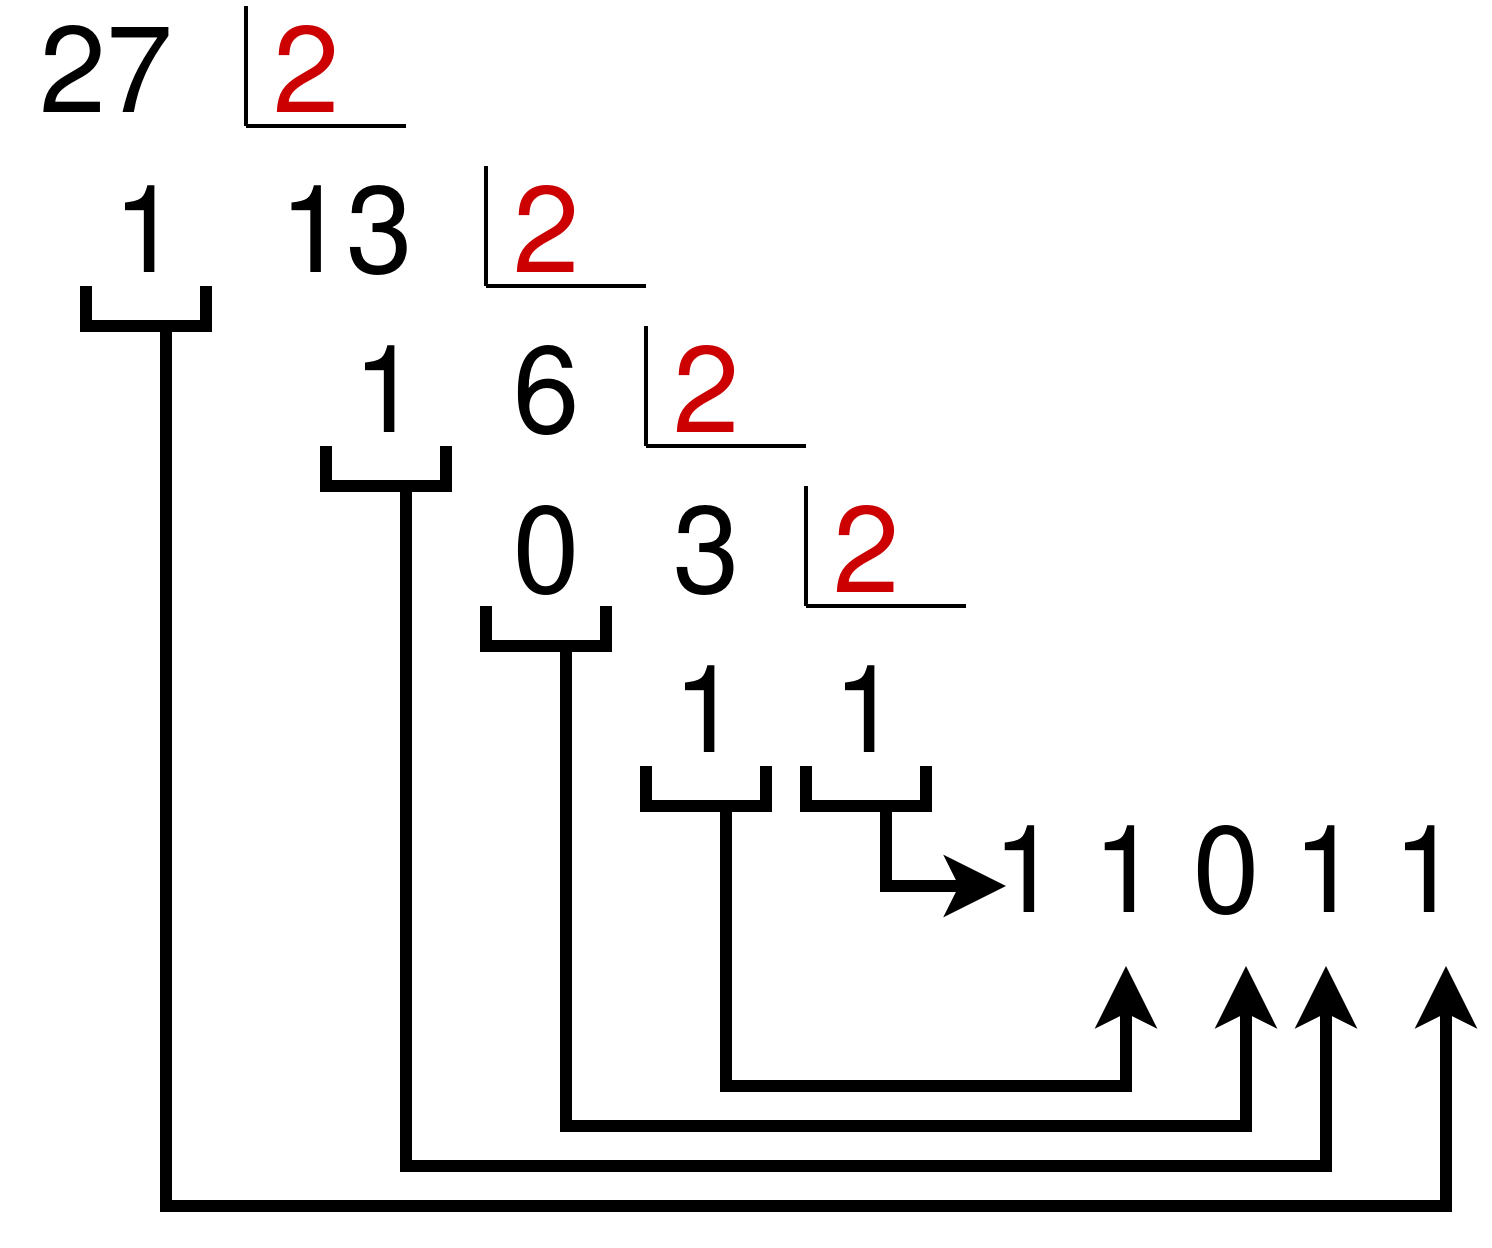
\includegraphics[width=0.29\linewidth]{decimal_binario.png}
    \vspace{-20pt}
\end{center}

\textbf{Los restos los cogemos en orden inverso} para obtener la siguiente equivalencia: $\mathbf{27_{(10} = 11011_{(2}}$

\subsection*{... hexadecimal}
Se trata de dividir sucesivamente el número decimal y los sucesivos cocientes entre 16 (la base hexadecimal). Cuando el cociente o resto sea entre 10 y 15, habrá que cambiarlo por la letra correspondiente.

\begin{center}
    \vspace{-10pt}
    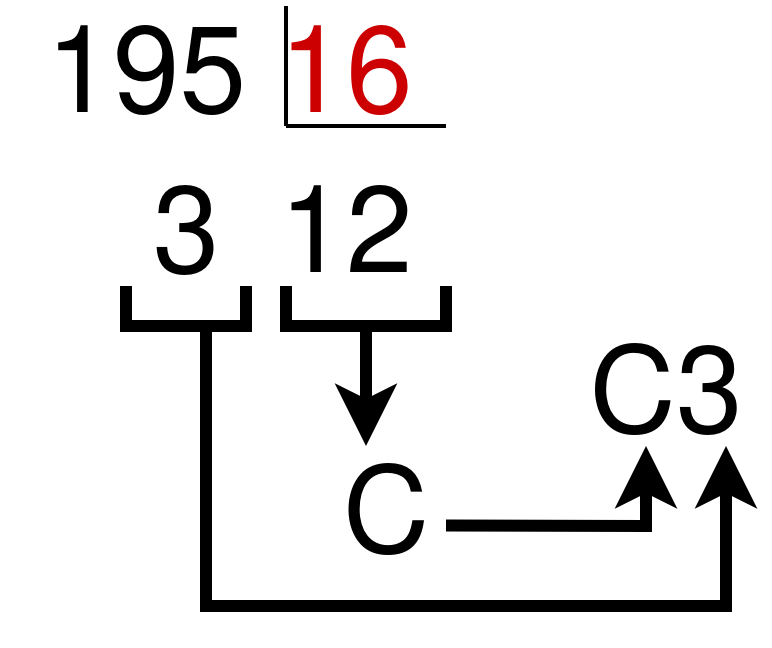
\includegraphics[width=0.2\linewidth]{decimal_hexadecimal.png}
    \vspace{-15pt}
\end{center}

\textbf{Los restos los cogemos en orden inverso} para obtener la siguiente equivalencia: $\mathbf{195_{(10} = C3_{(16}}$

\subsection*{... octal}
Al igual que los anteriores, hacemos divisiones sucesivas:

\begin{center}
    \vspace{-10pt}
    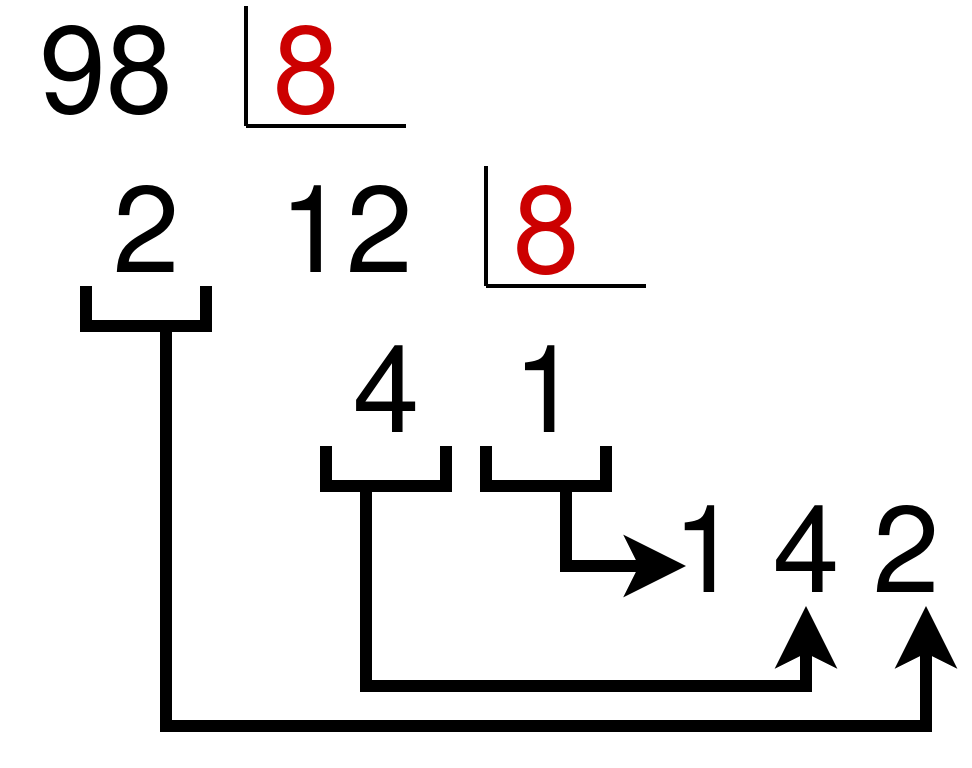
\includegraphics[width=0.25\linewidth]{decimal_octal.png}
    \vspace{-15pt}
\end{center}

\textbf{Los restos los cogemos en orden inverso} para obtener la siguiente equivalencia: $\mathbf{98_{(10} = 142_{(8}}$


\subsection{Conversión de binario a...}

\subsection*{... decimal}
El sistema de numeración binario es un sistema posicional donde cada dígito binario (bit) tiene un valor basado en su posición relativa al \textbf{LSB} (\textit{Least Significant Bit} = bit menos significativo, que es el que está más a la derecha y que tiene el menor valor).

Cualquier número binario puede convertirse a su equivalente decimal multiplicando cada bit por la base (2) y usando como exponente la posición (siendo 0 el exponente del bit de más a la derecha). Para ilustrarlo, cojamos como ejemplo el número binario $\mathbf{11011_{(2}}$:

\begin{center}
    \vspace{-20pt}

    $ \mathbf{11011_{(2}} $

    $ \mathbf{1\times2^4 + 1\times2^3 + 0\times2^2 + 1\times2^1 + 1\times2^0} $

    $ \mathbf{16 + 8 + 0 + 2 + 1 = 27_{(10}} $
    \vspace{-15pt}
\end{center}

Nótese que el procedimiento consiste en determinar los valores (es decir, las potencias de 2) de cada posición de bit que contenga un 1 y luego sumarlos.

Nótese también que el \textbf{MSB} (\textit{Most Significant Bit} = bit más significativo,\textbf{ el que está más a la izquierda}, el que tiene mayor valor) tiene un valor de $\mathbf{2^4}$ a pesar de que es el quinto bit. Esto se debe a que el \textbf{LSB} (\textit{Least Significant Bit}, el bit menos significativo, el que está a la derecha) es el primer bit y tiene un valor de $\mathbf{2^0}$.

\subsection*{... octal}
Para convertir un número binario a octal \textbf{se agrupan los dígitos de 3 en 3 empezando desde el lado derecho} hacia la izquierda, sustituyendo cada trío de dígitos binarios por su equivalente en octal.

Si en el lado izquierdo quedase algún bit “suelto” (sin formar un grupo de 3), se pueden poner “0” a la izquierda.

Cogemos como ejemplo el número binario $\mathbf{1100101001001_{(2}}$ para pasarlo a octal, haremos:

\begin{center}
    \vspace{-15pt}
    $\mathbf{001\ \ 100\ \ 101\ \ 001\ \ 001_{(2} = 14511_{(8}}$
    \vspace{-15pt}
\end{center}

\subsection*{... hexadecimal}
Similar al caso anterior, pero en este caso \textbf{la agrupación que se realiza debe de ser de 4 en 4 bits}. Si usamos el mismo ejemplo anterior $\mathbf{1100101001001_{(2}}$ :

\begin{center}
    \vspace{-15pt}
    $\mathbf{0001\ \ 1001\ \ 0100\ \ 1001_{(2} = 1949_{(16}}$
    \vspace{25pt}
\end{center}



\subsection{Conversión de hexadecimal a...}
\subsection*{... binario}
Para pasar de hexadecimal a binario convertiremos cada símbolo hexadecimal a 4 dígitos binarios.

\begin{center}
    \vspace{-15pt}
    $\mathbf{F17A_{(16} = 1111\ \ 0001\ \ 0111\ \ 1010_{(2}}$

    $\mathbf{1A4F_{(16} = 0001\ \ 1010\ \ 0100\ \ 111_{(2}}$
    \vspace{-15pt}
\end{center}


\subsection*{... decimal}
Al igual que hemos hecho con las conversiones previas a decimal, se podría realizar haciendo potencias de 16, pero se entiende que es más complicado de realizar.

Por lo tanto, \textbf{la manera más sencilla es pasar primero a binario} como acabamos de ver \textbf{y posteriormente convertir ese binario a decimal} como hemos visto previamente.

\subsection*{... octal}
Pasar primero a binario y después a octal.



\subsection{Conversión de octal a...}
\subsection*{... binario}
Cada dígito en octal se convierte en su representación en 3 bits:

\begin{center}
    \vspace{-15pt}
    $\mathbf{167_{(8} = 001\ \ 110\ \ 111_{(2}}$

    $\mathbf{253_{(8} = 010\ \ 101\ \ 011_{(2}}$
    \vspace{-15pt}
\end{center}
Los ceros de la izquierda se podrían quitar, ya que no alteran el valor.

\subsection*{... decimal}
Se puede realizar de dos maneras. La primera es hacer uso de potencias de 8 (similar al paso de pasar de binario a decimal, pero cambiando la base):

\begin{center}
    \vspace{-15pt}
    $\mathbf{157_{(8} = 1\times8^2 + 5\times8^1 + 7\times8^0 = }$

    $\mathbf{1\times64 + 5\times8 + 7\times1 = }$

    $\mathbf{64 + 40 + 7 = 111_{(10}}$

    Resultado: $\mathbf{157_{(8} = 111_{(10}}$
    \vspace{-15pt}
\end{center}

Con números grandes puede ser un poco complicado calcular las potencias de 8, por lo que \textbf{la alternativa es pasarlo primero a binario} como hemos visto, \textbf{y después pasarlo de binario a decimal}.

\subsection*{... hexadecimal}
La manera más sencilla es realizar la conversión primero a binario tal como hemos visto, y posteriormente pasar el número binario a hexadecimal como se ha visto previamente.

\section{Comprobar conversiones}

Podemos hacer uso de la calculadora del sistema Windows para comprobar si estamos realizando de manera correcta las conversiones. El problema es que por defecto sólo hace uso del sistema decimal. Para poder utilizar los sistemas de numeración que hemos aprendido, es necesario utilizar la versión “Programador”.

\begin{center}
    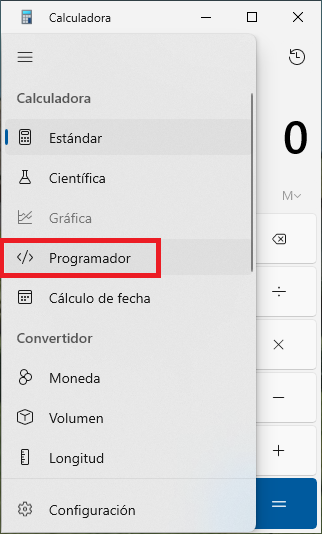
\includegraphics[width=0.45\linewidth]{calculadora1.png}
    \hfill
    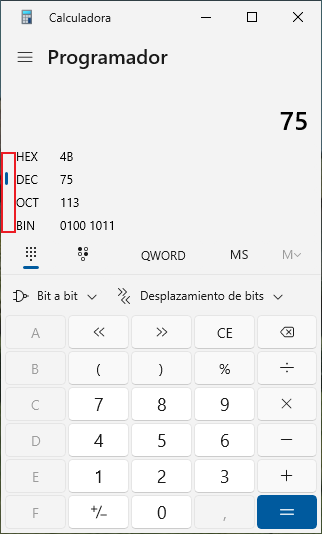
\includegraphics[width=0.45\linewidth]{calculadora2.png}
\end{center}

Una vez está en modo “Programador”, nos debemos fijar qué sistema de numeración está elegido. Al escribir cualquier número, en el resto de opciones veremos las conversiones automáticamente.

    \graphicspath{{../../../temas_comunes/unidades_informacion/img}}
    \chapter{Unidades de Información digital}

A la hora de almacenar información digital es importante conocer el tamaño del objeto que queremos almacenar y el espacio libre del lugar en el que lo queremos guardar.

En decimal estamos acostumbrados a contar usando el \href{https://es.wikipedia.org/wiki/Sistema_Internacional_de_Unidades}{Sistema Internacional de Unidades}, y dependiendo de la magnitud que queramos medir, haremos uso de unos prefijos establecidos. Por ejemplo, para medir la distancia usamos el \textbf{metro}, y por tanto nos quedaría:

\begin{itemize}
    \item \textbf{Sin prefijo} : metro, una unidad.
    \item \textbf{deca-}metro: $10^1$ metros
    \item \textbf{hecto-}metro: $10^2$ metros
    \item \textbf{kilo-}metro: $10^3$ metros
    \item \textbf{mega-}metro: $10^6$ metros
    \item \textbf{giga-}metro: $10^9$ metros
    \item ...
\end{itemize}

En decimal hacemos uso de la \textbf{base 10}, y por tanto  con cada prefijo lo que estamos haciendo es modificar el exponente que indica la cantidad. Para unidades pequeñas el exponente varía de uno en uno, pero a partir de cierta cantidad (\textbf{kilo-}), la cantidad cambia multiplicando por 1000 ($10^3$).


\section{Sistema binario}

En informática la información se guarda en formato binario, y la unidad más pequeña es el \textbf{bit}, que es un acrónimo de \textit{\textbf{bi}nary digi\textbf{t}}. Cada bit es una única unidad que sólo permite dos estados: \textbf{0} o \textbf{1}. A la hora de representarlo se hace uso de la letra \textbf{b} minúscula, por lo tanto, \textbf{10b} son 10bits.


\subsection{Múltiplos}

Al igual que en decimal, a medida que aumentamos la cantidad, se hace uso de prefijos para facilitar el conocer de qué cantidad estamos hablando.

A continuación se expone una tabla de las medidas más utilizadas:

\begin{yukitblr}{X X X}
    Nombre & Símbolo & Cantidad \\
    \textbf{Bit} & \textbf{b} & $2^0=1$ \\
    Nibble & & 4b \\
    \textbf{Byte} & \textbf{B} & 8b \\
    \textbf{Kibi}byte & \textbf{KiB} & $2^{10}=1024 B$ \\
    \textbf{Mebi}byte & \textbf{MiB} & $2^{20}=1024 KiB$ \\
    \textbf{Gibi}byte & \textbf{GiB} & $2^{30}=1024 MiB$ \\
    \textbf{Tebi}byte & \textbf{TiB} & $2^{40}=1024 GiB$ \\
    \textbf{Pebi}byte & \textbf{PiB} & $2^{50}=1024 TiB$ \\
    \textbf{Exbi}byte & \textbf{EiB} & $2^{60}=1024 PiB$ \\
\end{yukitblr}

Aunque esta es la manera correcta de nombrar las unidades cuando hablamos en términos informáticos, lo habitual es que se haga uso de los prefijos del sistema decimal.

\section{Usos}

A la hora de utilizar las medidas vistas previamente hay que diferenciar qué queremos medir, ya que no se hará siempre igual.

\begin{itemize}
    \item \textbf{Almacenamiento}: A la hora de querer expresar una cantidad de almacenamiento (para un disco duro, un \textit{pendrive} USB, RAM, ...) se hace uso del \textbf{Byte} y de sus múltiplos usando los prefijos vistos previamente.

    \begin{center}
        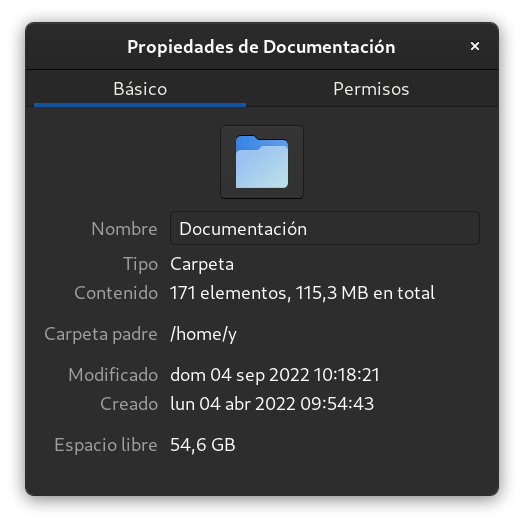
\includegraphics[width=0.4\linewidth]{hdd.png}
    \end{center}

    \item \textbf{Transmisión}: Cuando hablamos de tasa de transferencia de datos se hace uso del término “tasa de bits” (en inglés \textit{\textbf{bitrate}}), que indican el número de bits que se transmiten por unidad de tiempo. Hoy día se suele medir en kbps (o kb/s, kilobits por segundo), Mbps (Mb/s, o megabit por segundo), ... Para convertirlo a Bytes por segundo habría que dividirlo por “8”.

    \begin{center}
        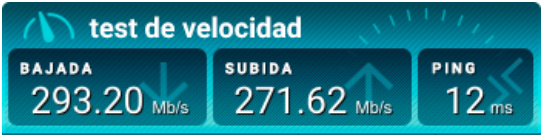
\includegraphics[width=0.4\linewidth]{bitrate.png}
    \end{center}

\end{itemize}

\warnbox{\textbf{La transmisión de datos se expresa en “bits por segundo”}}

    \vfill
    \pagebreak

    \part{Hardware y Software}
    \graphicspath{{img/si/}}
    \chapter{Introducción a Laravel}

\href{https://laravel.com/}{Laravel} es un \textit{framework} para crear aplicaciones y servicios web haciendo uso del lenguaje de programación \href{https://es.wikipedia.org/wiki/PHP}{PHP}, buscando la simplicidad y evitar el “\textit{spaghetti code}”. Hace uso de la arquitectura “modelo-vista-controlador” (MVS) y es un proyecto de código abierto.

\section{Características}
Entre las características que tiene Laravel, se pueden destacar:

\begin{itemize}
    \item Sistema de enrutamiento, también RESTful.
    \item Motor de plantillas web llamado \href{https://laravel.com/docs/10.x/blade}{Blade}. Nos permite:
    \begin{itemize}
        \item Crear plantillas que pueden incluir otras plantillas.
        \item Hacer uso de PHP dentro de las plantillas.
        \item Permite cachear las plantillas hasta que se modifiquen.
    \end{itemize}
    \item Creador de queries a la base de datos llamada \href{https://laravel.com/docs/10.x/queries}{Fluent}.
    \item \href{https://laravel.com/docs/10.x/eloquent}{Eloquent} como ORM (\textit{object-relational mapper}).
    \item Uso de “\textit{migrations}” para crear la base de datos a modo de sistema de control de versiones.
    \item Sistema de enrutado de la aplicación para relacionar rutas de acceso con controladores.
    \item Posibilidad de usar “semillas” (en inglés “\textit{seeds}”) en la base de datos para importar datos, ya sea de test o datos iniciales necesarios.
    \item Permite hacer uso de paquetes de \href{https://getcomposer.org/}{Composer}.
    \item Soporte para usar servicios de caché.
    \item Posibilidad de paginación automática.
\end{itemize}

Estas características las iremos utilizando para crear nuestro primer proyecto y para posteriormente aprender a crear una API que podrá ser accedida desde cualquier tipo de aplicación: un interfaz web, una aplicación móvil, desde línea de comandos...

    \chapter{Hardware}

Como ya se ha comentado previamente, el \textbf{hardware} es todo lo que forma parte del ordenador, que \textbf{puede ser tocado físicamente}. Dentro de un ordenador vamos a poder diferenciar distintos componentes que cumplirán una función distinta que detallaremos más adelante.

Es posible que ya conozcamos alguno de estos componentes, pero debemos conocer el origen y cómo surge la arquitectura de los ordenadores modernos.

\hypertarget{von_neumann}{}
\section{Arquitectura Von Neumann}

Las primeras computadoras electromecánicas eran diseñadas para un único propósito, estaban “diseñadas” para realizar una tarea. Un caso conocido puede ser \href{https://es.wikipedia.org/wiki/Bombe}{\textbf{Bombe}}, una máquina electromecánica capaz de descifrar los sistemas criptográficos nazis de Enigma. \movie{https://www.imdb.com/title/tt2084970/}{The Imitation Game}

Algunas se podían “reprogramar”, pero a base de recablear distintos componentes tras un estudio de lo que se quería realizar. Podía tomar hasta tres semanas preparar un programa de ENIAC y conseguir que funcionara.

El concepto de máquinas de computación universal y el uso de programa almacenado ya existía a nivel teórico desde mediados de la década de 1930 (escrito por \href{https://es.wikipedia.org/wiki/Alan_Turing}{Alan Turing}).

El matemático y físico \href{https://es.wikipedia.org/wiki/John_von_Neumann}{John von Neumann}, junto con otros compañeros, \textbf{describe en 1945 un diseño para una arquitectura de computadoras} en el que se describren los siguientes componentes que se interrelacionan entre sí a través del bus del sistema que actúa como canal de comunicación entre ellos:

\vspace{-10pt}
\begin{center}
    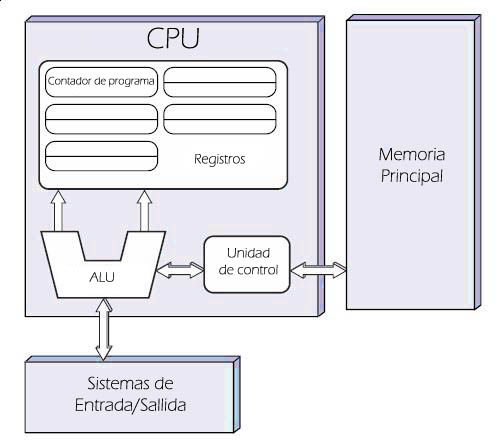
\includegraphics[width=0.5\linewidth]{vonneumann.jpg}
    \captionof{figure}{Arquitectura Von Neumann. Fuente: \href{https://es.wikipedia.org/wiki/Arquitectura_de_Von_Neumann}{wikipedia}}
\end{center}

\begin{itemize}
    \item \textbf{Unidad Central de Proceso} (\textbf{CPU}, por sus iniciales en inglés), que a su vez, contiene:
    \begin{itemize}
        \item \textbf{Unidad Aritmético Lógica} (\textbf{ALU} en inglés): Es un circuito digital que realiza operaciones aritméticas (suma, resta, multiplicaciones,...) y operaciones lógicas (AND, OR, X-OR,...) entre los valores de los argumentos (uno o dos).
        \item \textbf{Registros del procesador}: Memoria de alta velocidad y poca capacidad integrada en la CPU para almacenar datos utilizados durante la ejecución de un programa:
        \begin{itemize}
            \item Contador de programa
            \item Acumulador
            \item Registro de instrucciones
        \end{itemize}
        \item \textbf{Unidad de control}: Su función es buscar las instrucciones en la memoria principal, decodificarlas y ejecutarlas, empleando para ello la unidad de proceso.
    \end{itemize}
    \item La \textbf{memoria principal}: Sistema donde se almacenan las instrucciones y los datos del programa que se está ejecutando en ese instante, dividida en celdas que se identifican por medio de una única dirección.
    \item Los \textbf{sistemas de Entrada/Salida}: Realizan la transferencia de información entre periféricos de entrada y/o salida para extender las capacidades del equipo.
\end{itemize}


Hoy en día, los ordenadores han evolucionado, pero la arquitectura sigue siendo la misma, aunque más compleja.

\infobox{\textbf{Podemos ver una simulación de la Arquitectura Von Neumann \href{https://lab.xitrus.es/VonNeumann/}{aquí}}}


\section{Componentes básicos}

Un ordenador moderno se puede distinguir de distintos componentes, los cuales cumplen una función específica. Así mismo, también pueden contar con subcomponentes integrados que son necesarios para cumplir su cometido final.

A continuación se van a detallar los componentes necesarios de un ordenador moderno.

\hypertarget{placa_base}{}
\subsection{Placa base}

La placa base (conocida en inglés como \textit{motherboard}) es una tarjeta de circuito impreso que tiene elementos electrónicos (resistencias, condensadores, reguladoresm ...)  a la que se conectan el resto de componentes que forman el ordenador. Es por eso que se puede considerar como la parte fundamental a la hora de montar un ordenador, ya que sin ella, el resto de componentes no se podrán comunicar entre sí.


\subsubsection{Formatos de placa base}
Las placas base deben tener un tamaño compatible con las cajas en las que van a ir montadas, y es por eso que hay distintos tamaños estandarizados. Cada uno de estos tamaños determinan dónde van a ir montados algunos de los componentes y conectores, así como los agujeros donde irán los tornillos de sujeción a la caja.

Si queremos profundizar más en los distintos formatos, la \href{https://es.wikipedia.org/wiki/Placa_base#Formatos_de_placa_base}{Wikipedia} cuenta con una sección en la que se comparan los distintos tamaños.


\subsubsection{Conectores de la placa base}

Como ya hemos indicado, a la placa base se conectan el resto de componentes que forman el ordenador, y es por eso que va a tener distintos conectores:

\hypertarget{socket}{}
\begin{itemize}
    \item \textbf{Zócalo del microprocesador}: También llamado \textit{\textbf{socket}}. Es donde se conecta el microprocesador sin tener que soldarlo a la placa, y de esta manera puede ser sustituido. El número de conexiones que conectan la placa base al microprocesador ha ido aumentando a medida que ha ido evolucionando la tecnología, siendo hoy día de hasta 1700 conectores.

    Dependiendo del tipo de procesador, y el modelo, el socket variará en número de contactos y el tipo de los mismos. Existen distintas maneras de interconexión:
    \begin{itemize}
%        TODO: mejorar esto
        \begin{minipage}{0.6\linewidth}
            \setlength{\parskip}{1.2em}
            \item \textbf{PGA}: De \textit{ping grid array}, o matriz de rejilla de pines. El procesador cuenta con unos pines en formato perpendicular que se conectan al socket donde estarán unos agujeros.

            En la imagen se puede ver un Socket AM4 con tecnología PGA que tiene 1331 contactos.
        \end{minipage}
        \hfill
        \begin{minipage}{0.3\linewidth}
            \vspace{15pt}
            \hfill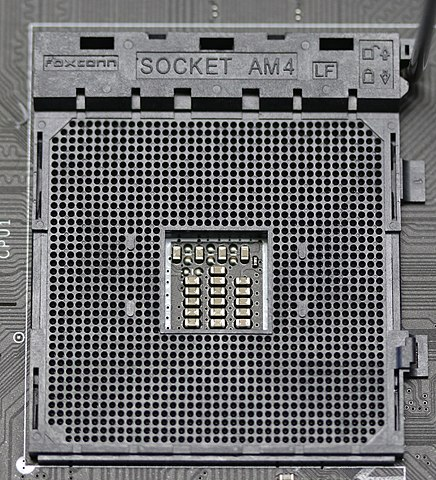
\includegraphics[width=\linewidth]{socket_pga.jpg}
        \end{minipage}
        \vspace{10pt}

        \begin{minipage}{0.6\linewidth}
            \setlength{\parskip}{1.2em}
            \item \textbf{LGA}: De \textit{land grid array}, o matriz de contactos en rejilla. En este caso el procesador \textbf{no cuenta} con pines, sino que es una matriz de contactos chapados en oro. Esta rejilla de contactos hacen contacto con el zócalo de la placa base que es la que cuenta con unos pequeños pines flexibles.
        \end{minipage}
        \hfill
        \begin{minipage}{0.3\linewidth}
            \hfill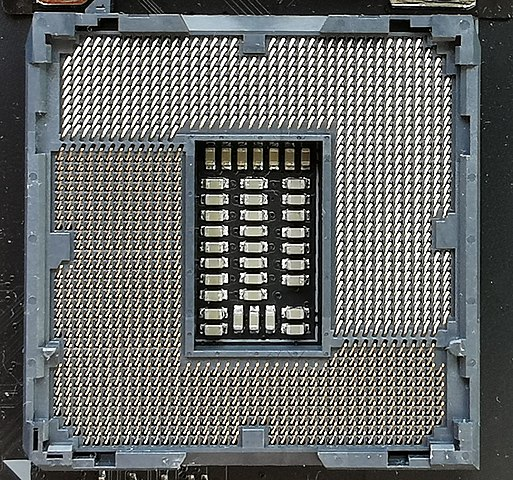
\includegraphics[width=\linewidth]{socket_lga.jpg}
        \end{minipage}
        \vspace{15pt}

        \item \textbf{BGA}: De \textit{ball grid array}, o matriz de rejilla de bolas. El procesador cuenta con unas bolas de estaño que al calentarse se sueldan a la placa base. Hoy en día se utiliza en componentes de tamaño reducido, como en móviles, los chips de memoria en los módulos de RAM, ...
    \end{itemize}

    \item \textbf{Conectores de alimentación}: La placa base tendrá distintos conectores provenientes de la fuente de alimentación con diferentes voltajes, para así proveer de alimentación a los componentes conectados a ella.

    \item \textbf{Ranuras de memoria RAM}: Hoy en día es habitual contar con varias ranuras donde conectar las memoria RAM. Más adelante hablaremos en profundidad sobre la memoria RAM.

    \item \textbf{Chipset}: Es un conjunto de chips, o circuitos electrónicos, que gestionan la comunicación entre los distintos componentes que forman el ordenador, y que están conectados en la placa base. Hoy en día se suelen dividir en dos partes:
    \begin{itemize}
        \item \textbf{Northbridge}: O puente norte. Controla el tráfico de los componentes que trabajan a más alta frecuencia. Comunica el microprocesador, la memoria RAM y la GPU (la ranura PCI express).
        \item \textbf{Southbridge}: O puente sur, comunica los periféricos, los dispositivos de almacenamiento, puertos de entrada/salida como USB, ethernet, ...
    \end{itemize}

    \item \textbf{Ranuras de expansión}: Vamos a identificar estas ranuras como las más modernas  \textbf{PCIexpress}. Son un bus de comunicación de datos de alta velocidad que es usado principalmente para conectar tarjetas gráficas.

    Es cierto que se pueden conectar otro tipo de tarjetas de expansión, como capturadoras de vídeo, tarjetas de red, controladoras RAID, ...

    Hoy en día existen conectores (\textbf{M.2}) donde poder conectar discos duros que tienen un tipo de conector especial.

    \item \textbf{Otros conectores de entrada/salida}: En la placa base existen otros muchos conectores de entrada y salida, que cumplirán distintas funciones dependiendo del tipo de conector, función y/o protocolo de comunicación que utilicen.

    Algunos de estos conectores tendrán conector exterior (al que se podrá conectar directamente el dispositivo), mientras que otros necesitarán de un adaptador (como sucede hoy día con conectores extra USB o el conector “serie”). Algunos ejemplos son:
    \begin{itemize}
        \item \textbf{USB}: Donde poder conectar distintos dispositivos como teclados, ratón, pendrives, mandos de juegos, impresoras, ... El USB (\textbf{Universal Serial Bus}) es un estándar de comunicación de periféricos hoy día. En las placas actuales también hay conectores de tipo \textbf{USB-C}.

        \item Conectores de \textbf{pantalla} como \textbf{VGA}, \textbf{HDMI} o \textbf{DisplayPort}. Dependiendo de lo moderna que sea la placa base, contará con uno o varios de estos conectores.

        \item \textbf{Red}: Hoy día el conector RJ45 es el estándar, que dependiendo de la versión ethernet, nos dará al menos 1Gbit de transmisión. Dependiendo del modelo de placa base también puede tener conectores para realizar conexiones a redes inalámbricas.

        \item \textbf{Audio}: Tanto de entrada como de salida. Normalmente se hace uso de conectores de tipo \textbf{jack}, pero también puede haber conectores de salida digital.

        \item \textbf{Pila}: Las placa base cuentan con una pila para mantener la alimentación para guardar la información de la RAM-CMOS, que es una pequeña memoria que usa la BIOS durante el arranque del sistema.

        \item \textbf{Conectores para ventiladores}: Para regular la temperatura del microprocesador y del interior de la caja, la placa tiene varios conectores que se conectarán a distintos ventiladores que se regularán en intensidad.

        \item \textbf{Otros conectores}: Existen otros conectores para otros puertos que hoy en día no se usan tanto (serie, paralelo, ...) y también los conectores para encender el ordenador, realizar el reset, comprobar el funcionamiento del disco...
    \end{itemize}

\end{itemize}

A continuación un diagrama simplificado de una placa base. Fuente: \href{https://es.wikipedia.org/wiki/Placa_base}{Wikipedia}.
\vspace{-10pt}
\begin{center}
    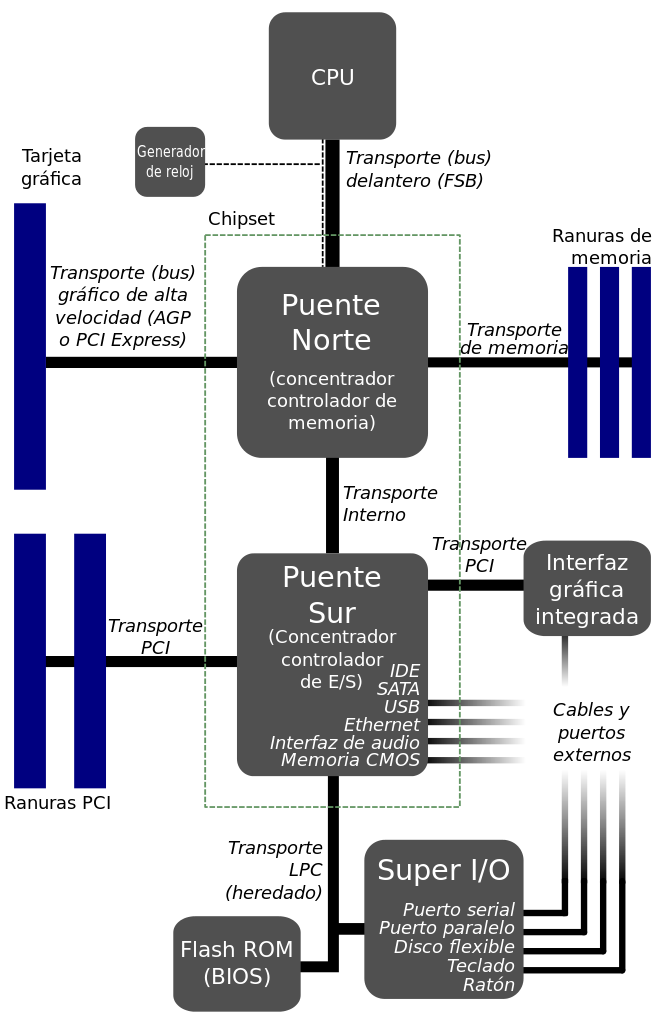
\includegraphics[width=0.56\linewidth]{placa_base_chipset.png}
\end{center}


\subsubsection{Ejemplo de placa base}

A continuación se van a diferenciar los componentes vistos anteriormente en una placa base real, utilizada para crear un equipo de escritorio moderno:

\begin{center}
    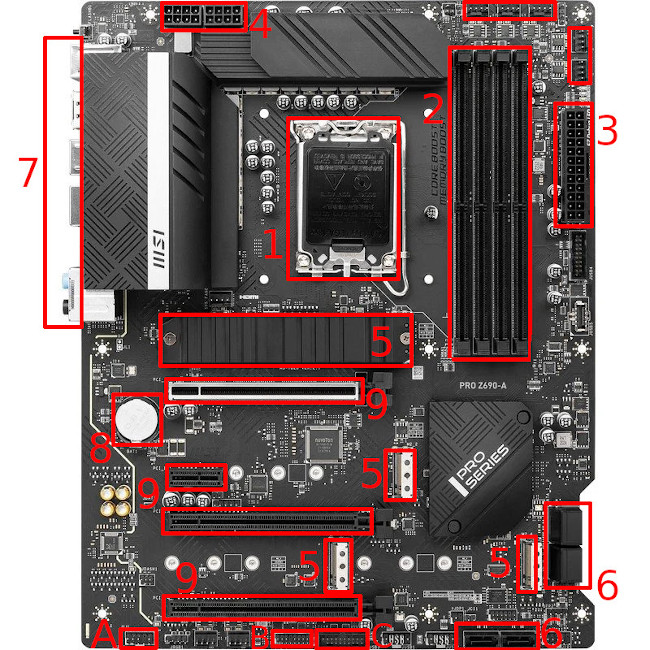
\includegraphics[width=\linewidth]{placa_base.jpg}
    \captionof{figure}{Placa Base MSI PRO Z690-A.  \href{https://download.msi.com/archive/mnu_exe/mb/M7D25v2.0.pdf}{Manual}}
\end{center}

\begin{enumerate}
    \item Zócalo (socket) del procesador.
    \item Ranuras para la memoria RAM.
    \item ATX de alimentación.
    \item Conectores de alimentación extra necesarios por la CPU.
    \item M.2 para discos duros.
    \item SATA para discos duros.
    \item Conectores exteriores (se verán a continuación)
    \item Pila.
    \item Ranuras PCIexpress de distintas velocidades.
    \item[A.] Audio
    \item[B.] Conectores frontales.
    \item[C.] USB 3.0
\end{enumerate}

Los conectores exteriores de esta placa tienen el siguiente aspecto:
\begin{center}
    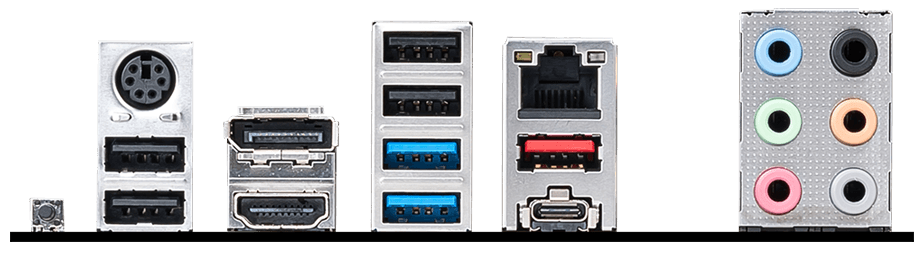
\includegraphics[width=\linewidth]{placa_base_frontal.png}
    \captionof{figure}{Placa Base MSI PRO Z690-A.  \href{https://download.msi.com/archive/mnu_exe/mb/M7D25v2.0.pdf}{Manual}}
\end{center}

De izquierda a derecha, y de arriba abajo:
\begin{itemize}
    \item Pulsador para actualizar la BIOS.
    \item Conector PS2 y USB para actualizar la BIOS.
    \item DisplayPort y HDMI
    \item Usb 2.0 y 3.2
    \item Conector LAN, USB y USB-C
    \item Conectores de audio
\end{itemize}


\subsection{BIOS/UEFI}
La BIOS/UEFI es un interfaz de firmware que está incorporado en un chip en la placa base.

La función principal es la de iniciar el ordenador, realizar una comprobación del \textit{hardware} del sistema  y se encarga de arrancar el gestor de arranque.

Se ha unificado en esta sección BIOS y UEFI ya que cumplen de manera similar la misma función, pero la segunda es una evolución de la primera.

\subsubsection{BIOS}

El sistema básico de entrada-salida (del inglés \textit{Basic Input/Output System}, o BIOS) lo creó IBM para sus ordenadores “\textbf{Personal Computer}”. Posteriormente se obtuvo por ingeniería inversa las funciones que realizaba tratando de buscar equipos  que fueran compatibles (denominados “PC-compatible”) y de esta manera convirtiéndose en un estándar de facto.

\begin{center}
    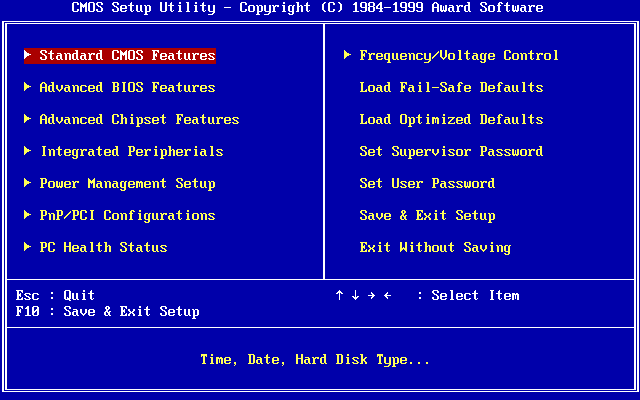
\includegraphics[width=0.7\linewidth]{bios.png}
    \captionof{figure}{Interfaz BIOS. Fuente \href{https://en.wikipedia.org/wiki/BIOS\#/media/File:Award_BIOS_setup_utility.png}{Wikipedia}}
\end{center}

A través de este interfaz se podían configurar algunos aspectos del hardware como las interrupciones de teclado que utilizaban los sistemas operativos antiguos (como MS-DOS), direcciones, el orden del sistema de arranque, ...


\hypertarget{UFI}{}
\subsubsection{UEFI}
La \textit{\textbf{Unified Extensible Firmware Interface}} (UEFI o «interfaz unificada de firmware extensible») es una especificación pública que define un interfaz entre el sistema operativo y el firmware de la plataforma.


\begin{center}
    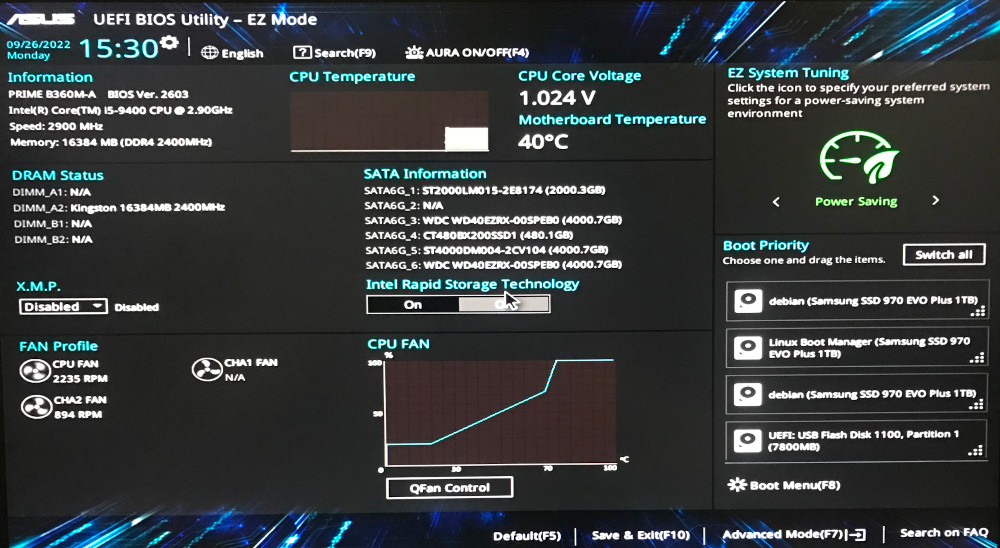
\includegraphics[width=0.7\linewidth]{uefi.jpg}
\end{center}

Se puede considerar una evolución de la BIOS  que tiene las siguientes características:

\begin{itemize}
    \item Permite arrancar desde particiones de más de 2TB gracias a eliminar las limitaciones del MBR (\textit{master boot record}).
    \item Diseño modular y extensible.
    \item Retro-compatible con BIOS.
    \item Interfaz gráfica más amigable con el usuario.
\end{itemize}


\subsection{Procesador}
El procesador (o microprocesador) es la unidad central de proceso (CPU) de la \hyperlink{von_neumann}{arquitectura Von Neumann}, y es el  circuito integrado más complejo que tiene el ordenador. Se puede considerar el “cerebro”.

Es el encargado de ejecutar todos los programas y operaciones que realizamos, pero sólo sabe ejecutar instrucciones en lenguaje máquina (código binario).

El microprocesador se conecta a la placa base a través del \hyperlink{socket}{socket}, y encima de él se añade un sistema de refrigeración para disipar el calor que genera durante su funcionamiento.


\subsubsection{Características}
A la hora de determinar las características principales que cuenta un procesador podemos destacar las siguientes:

\begin{itemize}
    \item \textbf{Frecuencia del reloj}: Es la cantidad de veces que los transistores internos del procesador pueden conmutar eléctricamente (abrir y cerrar el flujo de corriente eléctrica). Hoy en día se mide en GHz (gigahercios), donde 1GHz es mil millones de ciclos por segundo.

    Normalmente se confunde con el número de operaciones o instrucciones que puede ejecutar en un segundo, pero eso no es del todo correcto.

    Tampoco determina que cuanta mayor frecuencia el procesador vaya a ser mejor que otro con menor frecuencia (ya existían procesadores a 4GHz hace años).

    \item \textbf{Bus de direcciones}: Este tamaño determinará la cantidad máxima de memoria que podemos direccionar. Con 32 bits se pueden direccionar 2³², es decir, 4GB. Mientras que con 64 bits en los procesadores modernos llegamos hasta los 16 exabytes de memoria RAM (2⁶⁴).

    \item \textbf{Bus de datos}: Es el dato más grande que es capaz de manejar en una única instrucción.

    \item \textbf{Memoria caché}: Es una memoria que se encuentra internamente dentro del procesador, que es mucho más rápida, pero también de mucho menor tamaño, si la comparamos con la memoria RAM. Los procesadores actuales cuentan con unos pocos MB de tamaño dependiendo del nivel de caché. Ejemplo el \href{https://ark.intel.com/content/www/us/en/ark/products/134586/intel-core-i512400-processor-18m-cache-up-to-4-40-ghz.html}{Intel Core i5-12400} con 7.5MB de L2 caché.

    \item \textbf{Voltaje}: Para que el procesador funcione necesita ser alimentado con frecuencia eléctrica. Normalmente a mayor voltaje se consigue mayor frecuencia de reloj.

    \item \textbf{Número de cores}: Los microprocesadores actuales no cuentan con una única CPU interna (como era habitual hasta el año 2006 más o menos), ya que pueden contar con varias, denominadas “\textit{\textbf{cores}}”.

    Actualmente también se pueden diferenciar en el tipo de \textit{core} que tiene, ya que algunos están diseñados para más eficiencia mientras que otros para mayor carga de trabajo.

    \item \textbf{Multihilo/Hyperthreading}: Consiste en simular dos procesadores lógicos dentro de un único procesador físico. Permite ejecutar programas que están preparados, y eso permite una mejora en el rendimiento.
\end{itemize}


Existen otro tipo de características más técnicas, pero que también son importantes de conocer. A nivel de cómo está diseñado el procesador, lo que se denomina la \textbf{arquitectura interna} también contamos con diferencias. Hoy día podemos encontrar dos arquitecturas diferenciadas:
\begin{itemize}
    \item \textbf{CISC}: Del inglés \textit{Complex Instruction Set Computer} (conjunto de instrucciones complejas), es un conjunto de instrucciones  que se caracteriza por ser muy amplio y permitir operaciones complejas entre operandos situados en la memoria o en los registros internos.

    Los CISC pertenecen a la primera corriente de construcción de procesadores. Pertenecen a esta arquitectura la mayoría de los procesadores actuales de ordenadores personales: AMD, X86\_64.

    \item \textbf{RISC}: Del inglés \textit{Reduced Instruction Set Computer} (computador con conjunto de instrucciones reducido) es una filosofía de diseño de CPU para computadora que está a favor de conjuntos de instrucciones pequeñas y simples que toman menor tiempo para ejecutarse.

    Hoy en día podemos encontrar esta arquitectura sobre todo en \href{https://es.wikipedia.org/wiki/Arquitectura_ARM}{ARM} que se utiliza en procesadores de móviles como los A15 de Apple (pero también en los procesadores de escritorio M1 y M2), Qualcomm Snapdragon, ...

\end{itemize}



\subsubsection{Rendimiento}
Dadas todas las características que hemos visto previamente, no podemos determinar si un procesador es mejor a otro sólo mirando sus características y determinando que “cuanto más mejor”. Por ejemplo:

\begin{itemize}
    \item \textbf{Intel Pentium 4}: 2.80GHz de frecuencia de reloj
    \item \textbf{Intel Core 2 Duo E8200}: 2.66GHz de frecuencia de reloj
    \item \textbf{Intel i5-11400}: Frecuencia de reloj base 2.60GHz.
    \item \href{https://cpu.userbenchmark.com/Compare/Intel-Pentium-4-280GHz-vs-Intel-Core2-Duo-E8200/m3163vsm3200}{Comparativa entre los dos primeros}
    \item \href{https://cpu.userbenchmark.com/Compare/Intel-Core-i5-11400-vs-Intel-Core2-Duo-E8200/4112vsm3200}{Comparativa entre los dos últimos}
\end{itemize}

\errorbox{\textbf{No nos podemos quedar con la idea de que “cuanto más mejor” cuando nos referimos a cantidades en as características del procesador}}

Es por eso que existen las \textbf{pruebas de rendimiento}, también conocido en inglés como \textbf{benchmark}.

Estas pruebas de rendimiento se ejecutan a través de un programa que va a ejecutar un conjunto de operaciones (que siempre serán las mismas) y determinará el tiempo llevado a cabo, y junto con otras especificaciones terminará dando una puntuación al resultado obtenido.

De esta manera, si utilizamos el mismo programa de benchmark en dos procesadores distintos, obtendremos puntuaciones distintas. Por ejemplo, \href{https://www.geekbench.com/}{Geekbench} es un programa multiplataforma muy popular hoy día:

\begin{center}
    \vspace{-20pt}
    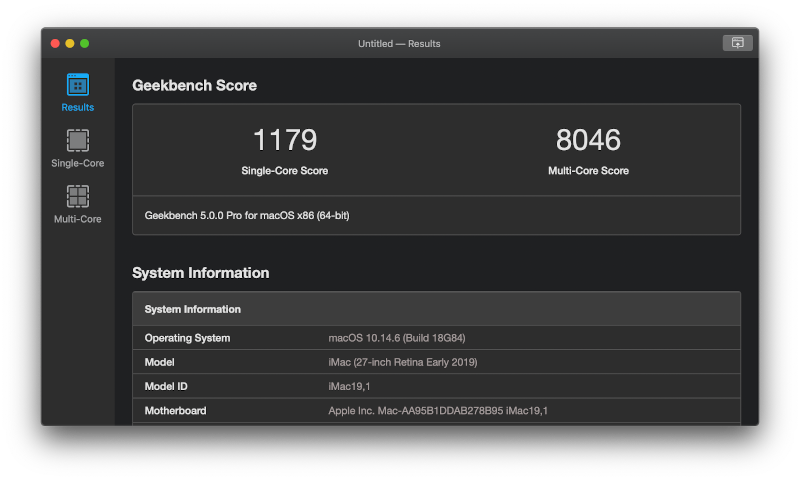
\includegraphics[width=0.8\linewidth]{geekbench.png}
    \vspace{-20pt}
\end{center}


\subsection{Sistema de refrigeración}
Debido a que el procesador genera calor durante su funcionamiento, y que esto repercute en su funcionamiento, se debe de mantener a una temperatura acorde. Es por ello que debemos hacer uso de un sistema de refrigeración.

El sistema de refrigeración cuenta con dos partes:
\begin{itemize}
    \item \textbf{Disipador}: Está en contacto con el procesador y por el \href{https://es.wikipedia.org/wiki/Principio_cero_de_la_termodin%C3%A1mica}{principio cero de la termodinámica} le traspasa el calor.
    \item \textbf{Sistema de reducción de temperatura}: Trata de reducir el calor que recibe el disipador para que el procesador se enfríe. Podemos diferenciar los siguientes sistemas:
    \begin{itemize}
        \item \textbf{Por aire}: Usando ventiladores.
        \item \textbf{De agua autocontenida y aire}: Es un circuito cerrado de agua que pasa a través de un radiador refrigerado por ventiladores. Venden el sistema cerrado, por lo que no hay que hacer nada con el líquido.
        \item \textbf{Refrigeración líquida}: Se utilizan componentes especiales para realizar el contacto con la CPU (y la GPU), y se debe hacer un circuito cerrado por el que pasará el líquido refrigerante, y una bomba que moverá el líquido.
    \end{itemize}
\end{itemize}

{
\hfill
\begin{minipage}{0.3\linewidth}
    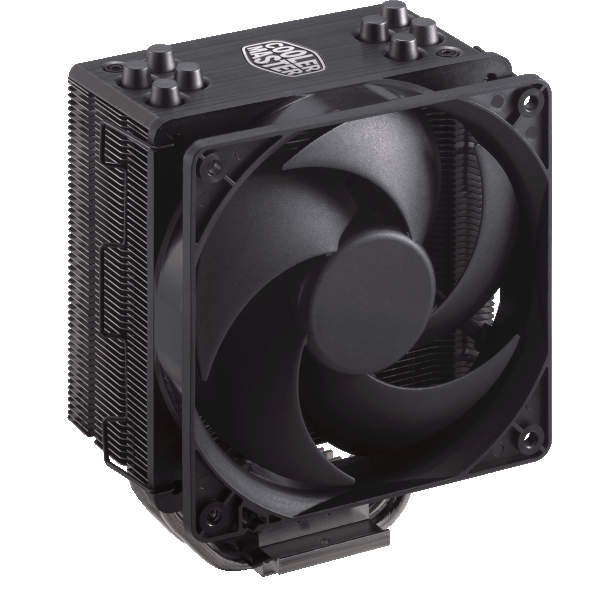
\includegraphics[width=\linewidth]{cooler_1.png}
\end{minipage}
\hfill
\begin{minipage}{0.5\linewidth}
    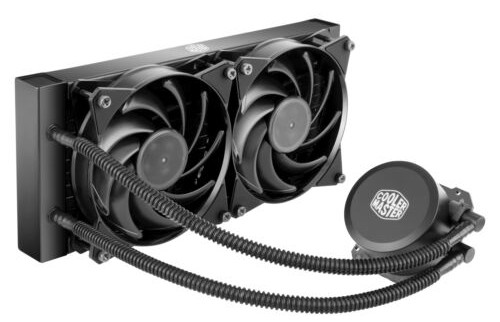
\includegraphics[width=\linewidth]{cooler_2.jpg}
\end{minipage}
\hfill
\vspace{30pt}
}


\subsection{Memoria RAM}

\begin{minipage}{0.6\linewidth}
\setlength{\parskip}{1.2em}
La memoria de acceso aleatorio (en inglés \textit{Random Access Memory}) es una memoria a corto plazo para almacenar los programas que están siendo ejecutados.

Cuando un programa se ejecuta se cargan todas sus instrucciones en RAM, así como todos los datos que va a manipular.

Es una memoria \textbf{volátil}, esto quiere decir que cuando deja de recibir electricidad, se pierde la información, por ejemplo al apagarse el ordenador o al reiniciarlo.

Se denominan “de acceso aleatorio” porque se puede leer o escribir en cualquier posición tardando lo mismo, no siendo necesario seguir un orden para acceder.

A lo largo de la \href{https://es.wikipedia.org/wiki/Memoria_de_acceso_aleatorio\#M%C3%B3dulos_de_RAM}{historia} la memoria RAM ha tomado distintas formas:
\end{minipage}
\hfill
\begin{minipage}{0.35\linewidth}
    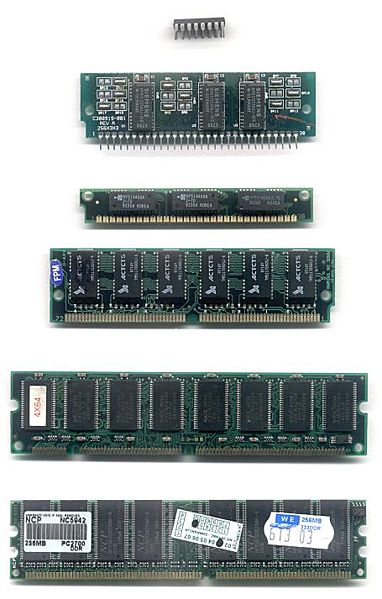
\includegraphics[width=\linewidth]{ram_evolution.jpg}
    \vspace{-30pt}
    \captionof{figure}{Fuente: \href{https://commons.wikimedia.org/wiki/File:RAM_n.jpg}{Wikipedia}}
\end{minipage}

\begin{itemize}
    \item Antes de los circuitos integrados era una matriz metálica que funcionaba por electromagnetismo. \href{https://es.wikipedia.org/wiki/Memoria_de_acceso_aleatorio#/media/Archivo:Electronic_Memory.jpg}{Foto}.
    \item Con la llegada de los circuitos integrados se instalaban en la placa soldandolos o sobre pequeños zócalos.
    \item Para hacer el sistema modular, se pasó al formato SIPP (\textit{Single In-line Pin Package}). En una sola tarjeta se integraban varios módulos de memoria, pero los pines eran frágiles.
    \item Como evolución llegó el formato SIMM (\textit{single In-line Memory Module}), que en lugar de pines tenía contactos en ambas caras del módulo.
    \item Hoy en día hacemos uso del formato DIMM (\textit{Dual In-line Memory Module}) y su versión reducida SO-DIMM utilizada en portátiles.
\end{itemize}

Hoy en día hacemos uso de memoria dinámica de acceso aleatorio que tiene un interfaz síncrona (SDRAM) y que tienen la capacidad de transferir simultáneamente datos por dos canales distintos en un mismo ciclo de reloj (DDR, de \textit{double data rate}).

A continuación se pueden diferenciar cómo ha variado el formato físico.

{
    \hfill
\begin{minipage}{0.45\linewidth}
    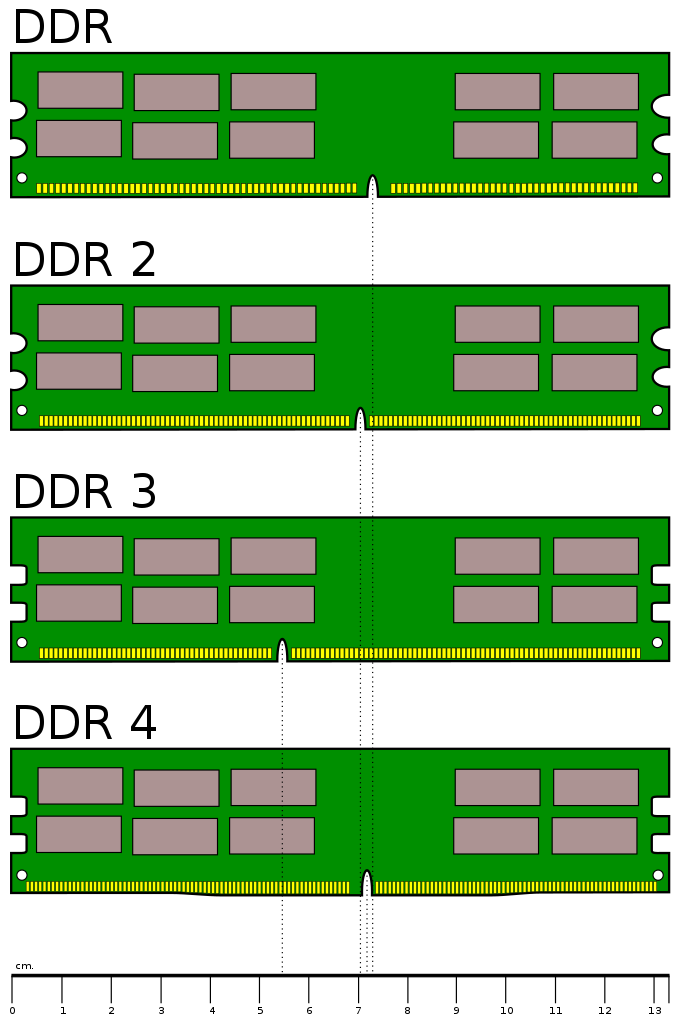
\includegraphics[width=\linewidth]{ddr.png}
    \vspace{-30pt}
    \captionof{figure}{Fuente: \href{https://commons.wikimedia.org/wiki/File:RAM_n.jpg}{Wikipedia}}
\end{minipage}
\hfill\hfill
\begin{minipage}{0.3\linewidth}
    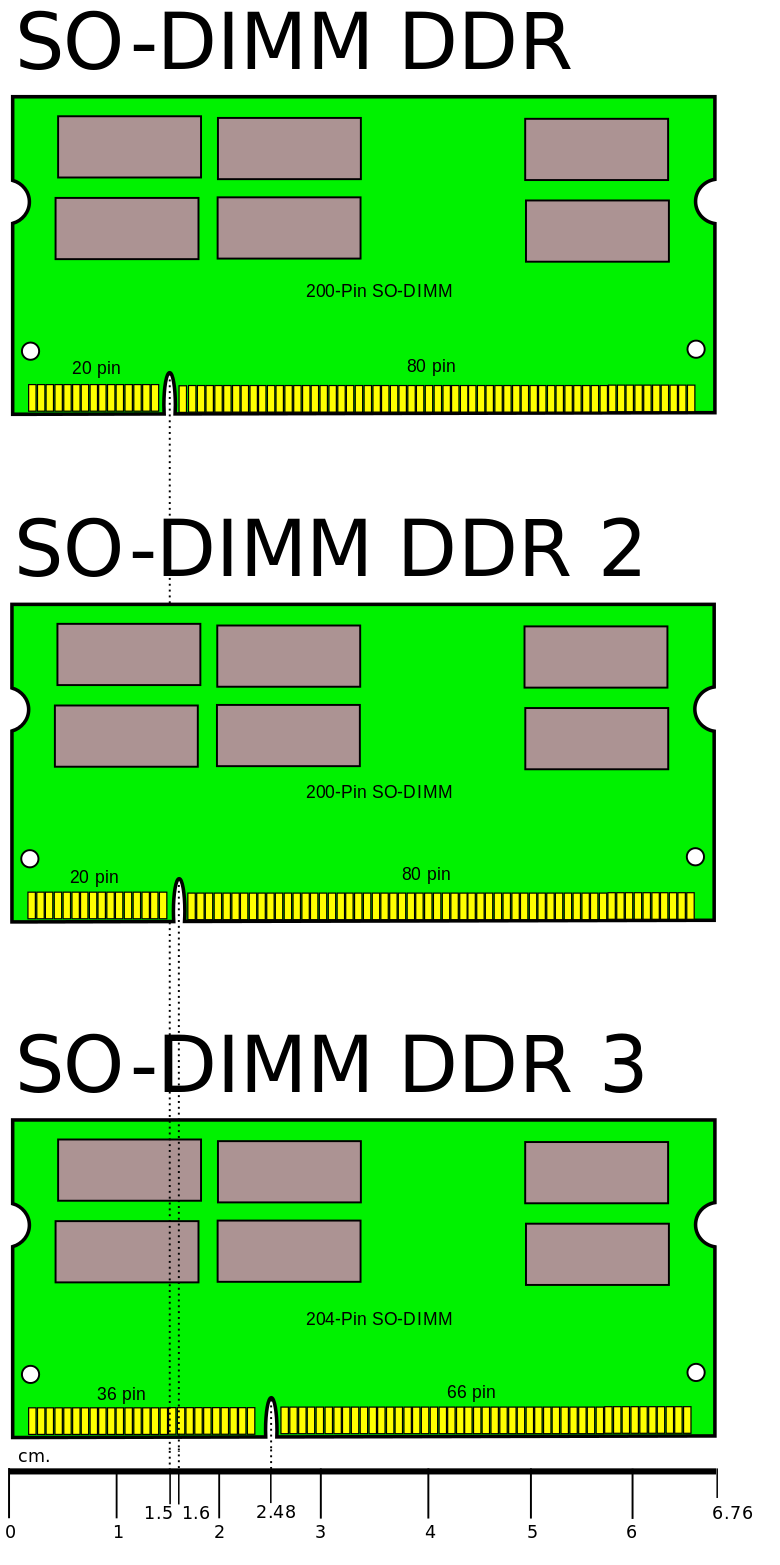
\includegraphics[width=\linewidth]{ddr_sodimm.png}
    \vspace{-30pt}
    \captionof{figure}{Fuente: \href{https://es.wikipedia.org/wiki/DDR_SDRAM}{Wikipedia}}
\end{minipage}
\hfill
}

En la \href{https://en.wikipedia.org/wiki/DDR_SDRAM#Generations}{Wikipedia} podemos ver una tabla con la evolución desde DDR hasta DDR5, con todos los datos técnicos como: voltaje utilizado, número de pines, ancho de banda en MB/s...

\hypertarget{dispositivos_almacenamiento}{}
\subsection{Dispositivos de almacenamiento de datos}

Los dispositivo de almacenamiento de datos nos permiten leer o grabar datos de forma temporal o permanente. Existen distintos tipos de dispositivos que se pueden diferenciar por formato, tamaño, tecnología, tipo de acceso, ...

Si diferenciamos por el tipo de tecnología utilizada para realizar el almacenamiento podemos distinguir:

\begin{itemize}
    \item \textbf{Dispositivos magnéticos}: Se utilizan las propiedades magnéticas de materiales para realizar el almacenamiento de datos digitales sobre el soporte de datos. En este apartado podemos poner como ejemplo:
    \begin{itemize}
        \item \href{https://es.wikipedia.org/wiki/Cinta_magn%C3%A9tica_de_almacenamiento_de_datos}{Unidades de cinta magnética}: No sólo utilizadas para almacenar datos en informática, también se ha utilizado en formato casete para la música.
        \item \href{https://es.wikipedia.org/wiki/Disquete}{Disquete}: O floppy disk, es un formato formado por una fina lamina circular dentro de una caja de plástico. Los tamaños más utilizados fueron de 8", 5 ¼" y 3½".
        \item \href{https://es.wikipedia.org/wiki/Unidad_de_disco_duro}{Discos duros}: Luego profundizaremos sobre ellos.
    \end{itemize}

    \item \textbf{Dispositivos ópticos}: Es un tipo de unidad de disco que utiliza un láser para realizar la lectura y escritura de datos. Los formatos más habituales en informática han sido los CDs, DVDs y Blu-Ray.

    \item \textbf{Unidad de estado sólido}: Conocidos como SSD (\textit{solid state drive}), hacen uso de memoria flash para almacenar datos de manera persistente.
\end{itemize}


Si diferenciamos por el acceso a los datos podemos diferenciar por:

\begin{itemize}
    \item \textbf{Acceso secuencial}: Para realizar la lectura del dato que nos interesa debemos leer registro a registro desde el inicio hasta llegar al dato que deseamos encontrar.

    \item \textbf{Acceso aleatorio}: Para realizar la lectura de un dato concreto, podemos acceder de manera directa, sin tener que pasar por el resto de datos.
\end{itemize}

Vamos a centrarnos en los denominados “discos duros” y que son  más utilizados a día de hoy:

\subsubsection{Discos duros HDD}

Las \href{https://es.wikipedia.org/wiki/Unidad_de_disco_duro}{unidades de discos duros} (también conocidos como HDD, de \textit{hard disk drive}) emplean un sistema de grabación magnética para almacenar y recuperar archivos digitales.

Están compuestos por varios \textbf{platos} de aluminio que giran todos a la vez sobre el mismo eje y que son recorridos por unos \textbf{cabezales} que están montados sobre unos brazos que recorren la superficie.

Estos cabezales son los encargados de magnetizar la superficie del plato al realizar las escrituras o leyendo la superficie para determinar cuál es el estado magnético y de esta manera conocer los datos guardados.

{
\begin{minipage}{0.57\linewidth}
        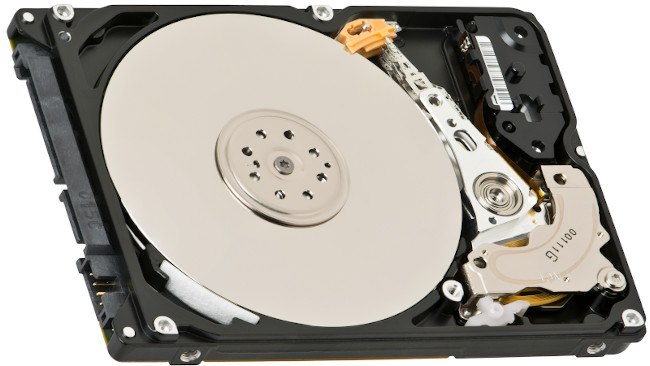
\includegraphics[width=\linewidth]{hdd.jpg}
\end{minipage}
\hfill
\begin{minipage}{0.42\linewidth}
    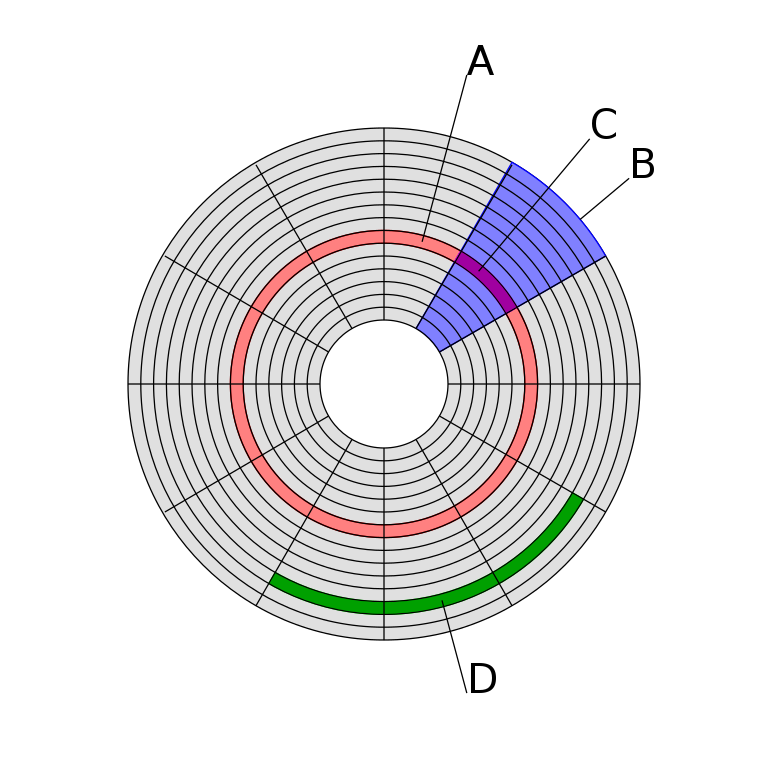
\includegraphics[width=\linewidth]{hdd_data.png}
\end{minipage}
\vspace{-35pt}
\begin{center}
  Fuente: \href{https://es.wikipedia.org/wiki/Unidad_de_disco_duro}{Wikipedia}
\end{center}
}

A la hora de guardar la información en los platos se sigue la estructura de la imagen superior, donde:

\begin{enumerate}
    \item[A.] Es una pista del disco.
    \item[B.] Es un sector geométrico.
    \item[C.] Es un sector de una pista.
    \item[D.] Es un grupo de sectores.
\end{enumerate}

%TODO: explicar cómo funciona

Si tenemos en cuenta las características que debemos tener en cuenta en un HDD, podemos destacar:

\begin{itemize}
    \item \textbf{Tiempo medio de acceso}: tiempo medio que tarda el cabezal en situarse en la pista y el sector deseado.
    \item \textbf{Tiempo de lectura/escritura}: tiempo medio que tarda el disco en leer o escribir nueva información: Depende de la cantidad de información que se quiere leer o escribir, el tamaño de bloque, el número de cabezales, el tiempo por vuelta y la cantidad de sectores por pista.
    \item \textbf{Velocidad de rotación}: Es la velocidad de giro de los platos. Por norma general a mayor velocidad de rotación, más alta será la transferencia de datos, pero también el ruido generado y el calor producido. Se mide en RPM (revoluciones por minuto). Dependiendo del tipo de disco puede variar entre 5.400RPM en equipos portátiles a 15.000RPM para servidores.
\end{itemize}

Debido a que los discos duros utilizan partes mecánicas hay que tener cuidado al transportarlos (aunque estén parados) y con el movimiento, ya que un golpe puede romper algún componente interno.

\errorbox{\textbf{Los discos duros HDD son propensos a golpes, debido a los componentes móviles internos}}

\subsubsection{SSD}

Conocidos como \textit{solid state drive}, hace uso de memorias \href{https://es.wikipedia.org/wiki/Memoria_flash}{flash} para el almacenamiento de datos en lugar de platos, y debido a que no tiene componentes móviles, son menos propensos a daños por golpes.

Debido a la mejora en la tecnología de guardado de datos, y por no poseer partes móviles, no generan ruido, son más ligeros, el tiempo de acceso a los datos es menor, y todo ello hace que la transferencia de datos aumente en comparación con los HDD.

{
    \begin{minipage}{0.48\linewidth}
        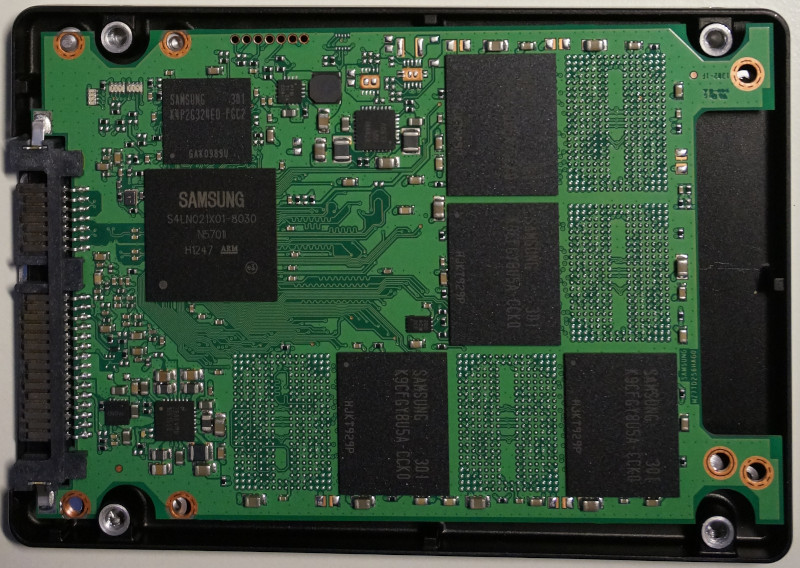
\includegraphics[width=\linewidth]{ssd.jpg}
    \end{minipage}
    \hfill
    \begin{minipage}{0.48\linewidth}
        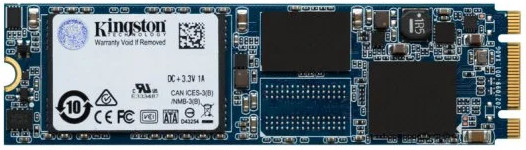
\includegraphics[width=\linewidth]{ssd2.jpg}
    \end{minipage}
    \vspace{-10pt}
    \begin{center}
       \footnotesize{Izquierda: Interior de SSD de 2,5”. Derecha: SSD conector m.2}
    \end{center}
}

Hoy en día la manera más habitual de usar este tipo de unidades es con el factor de forma de 2,5” o en conocido como mSATA o m.2.


\hypertarget{nvme}{}
\subsubsection{NVMe}
La especificación de interfaz de controlador de host de memoria no volátil (NVMHCIS, en inglés \textit{non-volatile memory host controller interface specification}) que está conectado a través del bus PCI Express (PCIe). Normalmente se llama NVMe para abreviar.

Este tipo de dispositivos, al igual que el anterior, hacen uso de tecnología FLASH para el almacenamiento de datos. Debido a que están conectados al bus PCI Express, y que la especificación de acceso se creó desde cero (para aprovechar la tecnología moderna de memorias FLASH, el paralelismo de las CPUs...), consiguen un rendimiento muy superior a las generaciones anteriores.

{
    \hfill
    \begin{minipage}{0.42\linewidth}
        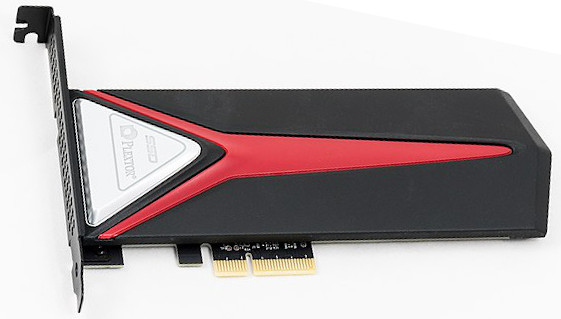
\includegraphics[width=\linewidth]{nvme1.jpg}
    \end{minipage}
    \hfill
    \begin{minipage}{0.35\linewidth}
        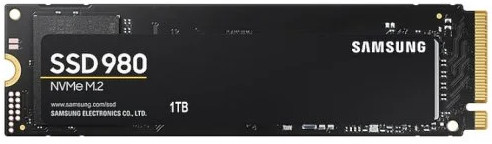
\includegraphics[width=\linewidth]{nvme2.jpg}
    \end{minipage}
    \hfill
    \vspace{-10pt}
    \begin{center}
        \footnotesize{Izquierda: NVMe en formato tarjeta PCIe. Derecha: NVMe con conector m.2}
    \end{center}
}

Las primeras unidades tenían un formato de tarjeta de expansión que se conectaba directamente a la ranura PCIexpress, mientras que hoy día existen los conectores M.2 para instalarlos.

\subsubsection{Comparativa HDD, SSD y NVMe}
En la siguiente tabla se puede comparar algunas características básicas de los distintos tipos de unidades de almacenamiento vistas.

\begin{yukitblrcol}{XXXXXX}
    & HDD & SSD & SSD (M.2)  & NVMe \linebreak (PCIe 3.0) & NVMe \linebreak (PCIe 4.0)\\
    Conector & SATA & SATA & M.2 & M.2  & M.2\\
    Velocidad Lectura & 150MB/s & 560 MB/s & 560 MB/s & 3500 MB/s & 7000 MB/s\\
    Velocidad Escritura & 120MB/s & 510 MB/s  & 520 MB/s &  3000 MB/s & 5300 MB/s\\
    Precio por TB & Bajo & Medio & Medio &  Alto & Alto\
\end{yukitblrcol}

Hay que tener en cuenta que las velocidades dependen de la tecnología de la unidad y también de la conexión utilizada. Son velocidades aproximadas, y por tanto habría que ver las especificaciones técnicas de cada dispositivo antes de comprarlo.

\infobox{Con las velocidades de lectura y escritura suelen indicar si es \textbf{secuencial} o \textbf{aleatoria}. \textbf{En lecturas y escrituras aleatorias la velocidad es más baja.}}

También existen pruebas de rendimiento para sistemas de almacenamiento, por lo que es importante informarse bien antes de elegir uno.


\subsection{Fuente de alimentación}

La fuente de alimentación en un ordenador es el componente que convierte la corriente alterna a varias corrientes continuas ya que el ordenador hace uso de diferentes voltajes.

A la hora de elegir una fuente de alimentación debemos tener en cuenta:

\begin{itemize}
    \item \textbf{Potencia}: Se mide en vatios (W, de \textit{watts}), y tendremos que tener en cuenta el consumo de los distintos componentes que tienen nuestro ordenador.
    \item \textbf{Factor de forma}: En los ordenadores de sobremesa hoy en día el formato es ATX, pero podemos elegir dependiendo del tipo de conexiones:
    \begin{itemize}
        \item \textbf{Cableado completo}: La fuente de alimentación cuenta con todo el cableado completo.
        \item \textbf{Semi-modular}: Algunos de los cables que son necesarios se pueden poner y quitar, dependiendo de las necesidades que tengamos.

        \item \textbf{Full-modular}: Todos los cables se pueden poner y quitar, lo que facilita la instalación de la fuente de alimentación y el orden dentro de la caja durante el montaje
    \end{itemize}
\end{itemize}
\vspace{15pt}
{
    \hfill
    \begin{minipage}{0.3\linewidth}
        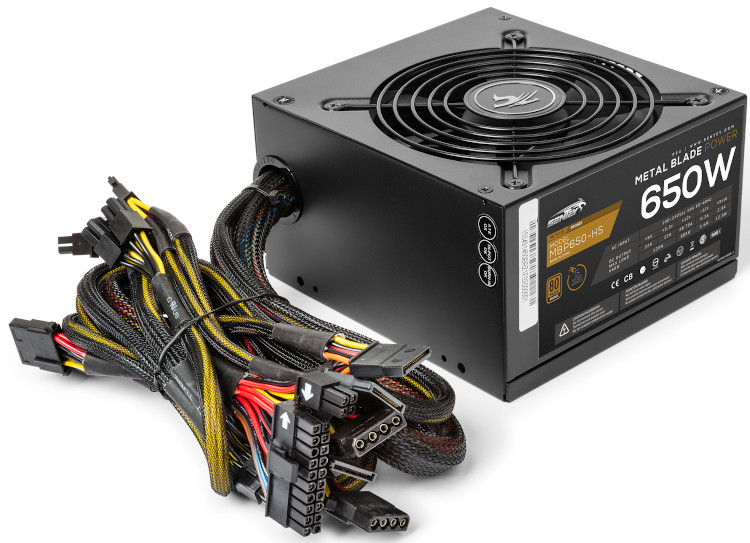
\includegraphics[width=\linewidth]{fuente_alimentacion_1.jpg}
    \end{minipage}
    \hfill
    \begin{minipage}{0.28\linewidth}
        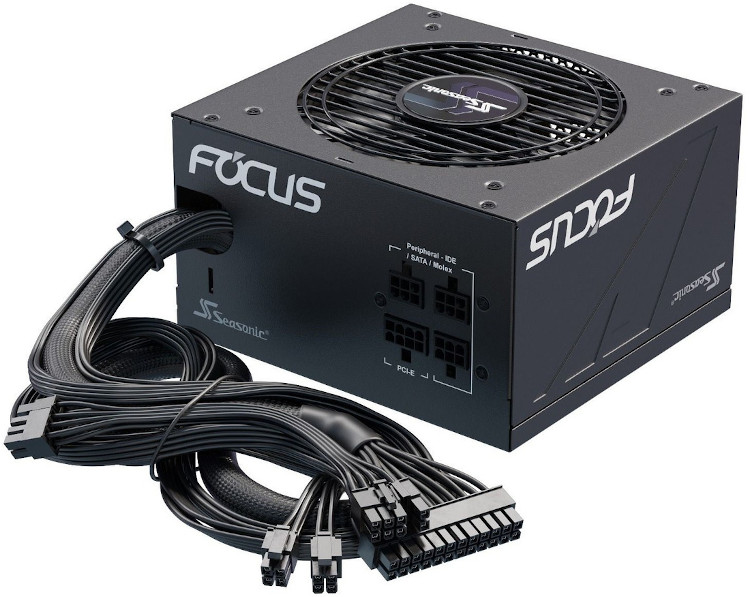
\includegraphics[width=\linewidth]{fuente_alimentacion_2.jpg}
    \end{minipage}
    \hfill
    \begin{minipage}{0.24\linewidth}
        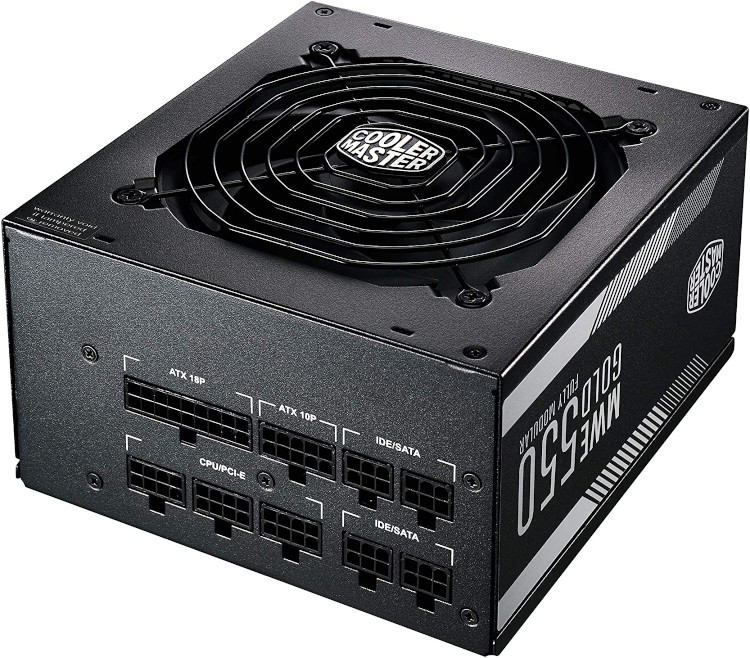
\includegraphics[width=\linewidth]{fuente_alimentacion_3.jpg}
    \end{minipage}
    \vspace{-10pt}
\begin{center}
     \footnotesize{Fuentes de alimentación con cableado completo, semi-modular y full-modular.}
\end{center}
}

\subsection{GPU/Tarjeta gráfica}
Hoy en día es habitual contar con una tarjeta gráfica en los ordenadores personales, cuando el desempeño de su función va a requerir realizar grandes procesamientos de gráficos como: juegos, edición de vídeo, edifición fotográfica, uso de dibujo asistido por ordenador, ...


Podemos diferenciar:

\begin{itemize}
    \item \textbf{Gráficos integrados}: Hoy en día los procesadores pueden contar con una unidad de procesamiento gráfico interna, que para el desempeño del uso del ordenador y tareas livianas (ver vídeos, juegos antiguos o con pocas necesidades) puede ser suficiente.

    Para confirmar si nuestro procesador tiene o no, deberíamos mirar las especificaciones técnicas del mismo (por ejemplo: \href{https://www.intel.com/content/www/us/en/products/sku/134595/intel-core-i712700kf-processor-25m-cache-up-to-5-00-ghz/specifications.html}{Intel i7-12700KF} no cuenta con procesador gráfico mientras que el \href{https://www.intel.com/content/www/us/en/products/sku/134591/intel-core-i712700-processor-25m-cache-up-to-4-90-ghz/specifications.html}{i7-12700} sí).

    \item \textbf{Gráficos dedicados}: Este es el caso de las denominadas tarjetas gráficas, que van conectadas a una ranura PCI-express. \textbf{Nos vamos a centrar en este tipo de tarjetas}.
\end{itemize}

Las tarjetas gráficas actualmente se instalan en la ranura PCI-Express de mayor velocidad de la placa base y suele contar con los siguientes componentes:

\begin{itemize}
    \item \textbf{Unidad de procesamiento gráfico}: O \textbf{GPU}, es un procesador como la CPU pero diseñado para el procesamiento gráfico. Su finalidad es la de realizar operaciones con vectores, triángulos, texturas, ... lo más rápido posible.

    Las tarjetas gráficas también sirven para realizar codificación/decodificación de vídeo por hardware, lo que disminuye el tiempo en comparación a realizar esa compresión a través de la CPU.

    Actualmente la tecnología puntera trata de simular la luz de la manera más real posible haciendo uso del denominado \href{https://es.wikipedia.org/wiki/Trazado_de_rayos}{raytracing}.

    \item \textbf{VRAM}: O memoria gráfica, son los chips que almacena y transporta información hacia la tarjeta gráfica. En el caso de las tarjetas gráficas dedicadas, cuentan con sus propios chips en la tarjeta, mientras que cuando hablamos de gráficos integrados suele ser RAM que se reserva para el uso de gráficos.

    \item \textbf{Conectores de salida}: Para poder realizar la conexión entre la tarjeta y los monitores que tengamos conectados. Hoy en día lo más habitual es tener conectores HDMI y DisplayPort.
\end{itemize}

Si nuestro procesador cuenta con una gráfica integrada y aparte tenemos una gráfica dedicada, dependiendo del uso que queramos darle al ordenador, quizá sea conveniente desactivar la integrada a través de la \hyperlink{UEFI}{UEFI}.

\infobox{Si tenemos gráfica integrada y dedicada, quizá nos interese desactivar la integrada a través de UEFI}

Las compañías que crean las tarjetas gráficas también han creado \textbf{SDK} (\textit{Software Development Kits}, o kits de desarrollo de software), como \href{https://en.wikipedia.org/wiki/CUDA}{Nvidia CUDA}, para poder realizar computación paralela y así aprovechar la potencia de cálculo para proyectos de \textit{machine learning},  simulaciones científicas, cálculo de proteínas, secuencias de ADN, ...

\infobox{\textbf{Podemos usar el procesamiento de la tarjeta gráfica para ayudar a la ciencia usando proyectos como \href{https://es.wikipedia.org/wiki/Folding@home}{Folding@Home} gracias a la \href{https://es.wikipedia.org/wiki/Computaci\%C3\%B3n_distribuida}{computación distribuida}}}


\subsection{Conectores más importantes}

Aunque ya hemos visto de manera generalizada algunos tipos de conexiones que tiene la placa base, vamos a profundizar en este apartado separándolos por secciones.

\subsubsection{Conectores gráficos}
Al igual que el resto de componentes, los conectores para dispositivos gráficos (pantallas) han sufrido una evolución, y aunque alguno de ellos tiene muchos años, hoy día se sigue utilizando.

 \begin{minipage}{0.15\linewidth}
    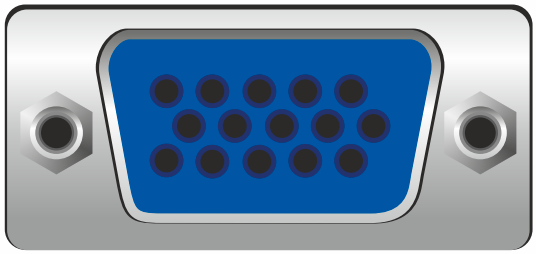
\includegraphics[width=\linewidth]{vga.png}
\end{minipage}
\hfill
\begin{minipage}{0.8\linewidth}
     El conector \textbf{VGA} es un conector analóigico que sólo envía la señal gráfica al dispositivo conectado. Hoy día, aunque se puede considerar obsoleto a nivel tecnológico, sigue estando presente en servidores y en proyectores de gama baja, ya que ofrece la suficiente calidad gráfica.
\end{minipage}


\vspace{12pt}
\begin{minipage}{0.15\linewidth}
   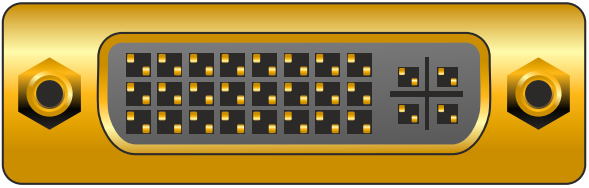
\includegraphics[width=\linewidth]{dvi.png}
\end{minipage}
\hfill
\begin{minipage}{0.8\linewidth}
   El conector \textbf{DVI} era el sucesor del conector anterior, y podía ser retrcompatible con VGA, aunque la idea es que este conector permitía tener señales digitales. Había diferentes tipos de conectores, dependiendo del tipo de señal que transportaba. Para portátiles también existió una versión “mini” y otra “micro”, que era más delgada.
\end{minipage}


\vspace{12pt}
\begin{minipage}{0.15\linewidth}
    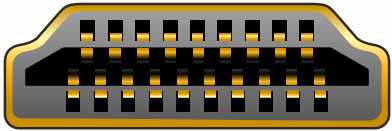
\includegraphics[width=\linewidth]{hdmi.png}
\end{minipage}
\hfill
\begin{minipage}{0.8\linewidth}
    El conector \textbf{HDMI} hoy en día es un estándar muy utilizado, sobre todo en televisiones, ya que permite enviar la señal gráfica y audio. Aunque el conector se mantiene igual, existen distintas revisiones que permiten mayor transmisión de datos (para tecnologías nuevas como HDR, audio con más canales, ...)
\end{minipage}

\vspace{12pt}
\begin{minipage}{0.15\linewidth}
    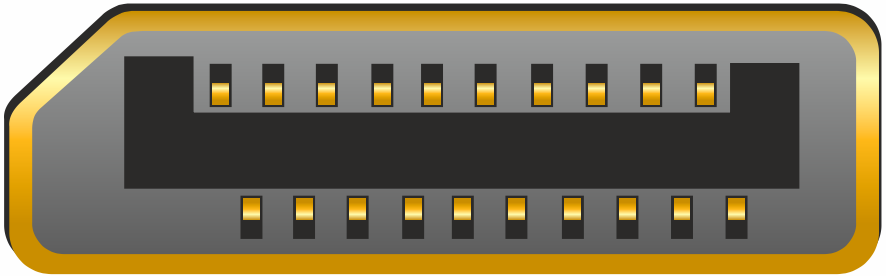
\includegraphics[width=\linewidth]{displayport.png}
\end{minipage}
\hfill
\begin{minipage}{0.8\linewidth}
    \textbf{DisplayPort} es un interfaz digital desarrollado por la Asociación de Estándares Electrónicos de Vídeo (VESA). Es libre de licencias, y opcionalmente permite la transmisión de audio y datos (por ejemplo USB).
\end{minipage}


\subsubsection{Conectores de dispositivos de almacenamiento}

Para dispositivos de almacenamiento, como discos duros, CD-ROMs... ha habido varios tipos de conectores que es importante conocer.

\begin{minipage}{0.15\linewidth}
    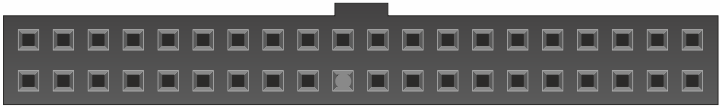
\includegraphics[width=\linewidth]{ide.png}
\end{minipage}
\hfill
\begin{minipage}{0.8\linewidth}
    \textbf{Parallel-ATA}, o IDE, era un conector que se utilizaba en discos duros y lectores de CD-ROM, con el que a través de un único cable podían conectarse dos dispositivos. Debido a esto, los dispositivos tenían un “\textit{jumper}” que identificaba si era el “maestro” o “esclavo”.
\end{minipage}

\begin{center}
    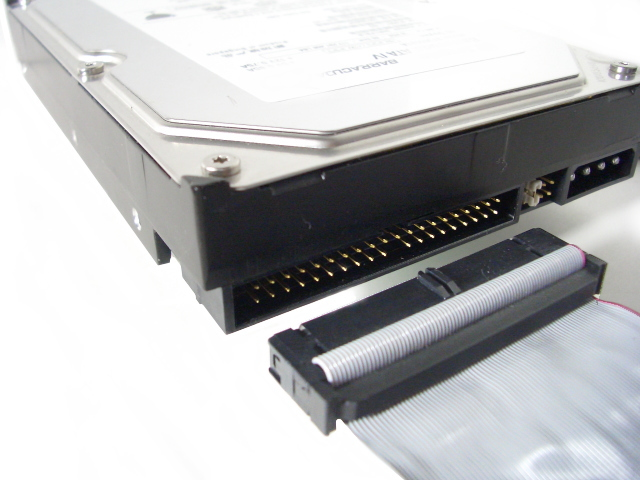
\includegraphics[frame,width=0.6\linewidth]{ide_hdd.jpeg}
    \captionof{figure}{Disco duro, cable IDE y jumper. Fuente: \href{https://commons.wikimedia.org/wiki/File:P-ata_and_80pin-cable.jpg}{wikipedia}}
\end{center}


\begin{minipage}{0.15\linewidth}
    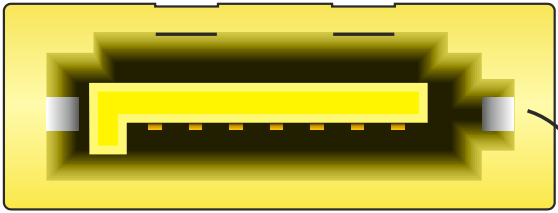
\includegraphics[width=\linewidth]{sata.png}
\end{minipage}
\hfill
\begin{minipage}{0.8\linewidth}
    \textbf{Serial-ATA}, o SATA, es la evolución del conector anterior. Es un conector más pequeño pero que permite más velocidad. Ha habido distintas versiones (siendo todas retrocompatibles), siendo la última SATA 3 (subversión 3.5), que admite hasta 600MB/s.
\end{minipage}


\begin{minipage}{0.15\linewidth}
    
\includegraphics[width=\linewidth]{m2.png}
\end{minipage}
\hfill
\begin{minipage}{0.8\linewidth}
    \textbf{M.2}, es el nuevo conector que incluyen los nuevos discos duros de estado sólido \textbf{\hyperlink{nvme}{NVMe}}.
\end{minipage}


\subsubsection{USB}

El USB (\textit{Universal Serial Bus}) es un estándar que define los cables, conectores y protocolos que más se utiliza hoy en día para conectar ordenadores y una infinidad de tipos de dispositivos.

Aunque se creó a mediados de los 90, su conector más utilizado (el tipo-A) apenas ha variado (buscando ser retrocompatible), pero sí su velocidad.

\begin{center}
    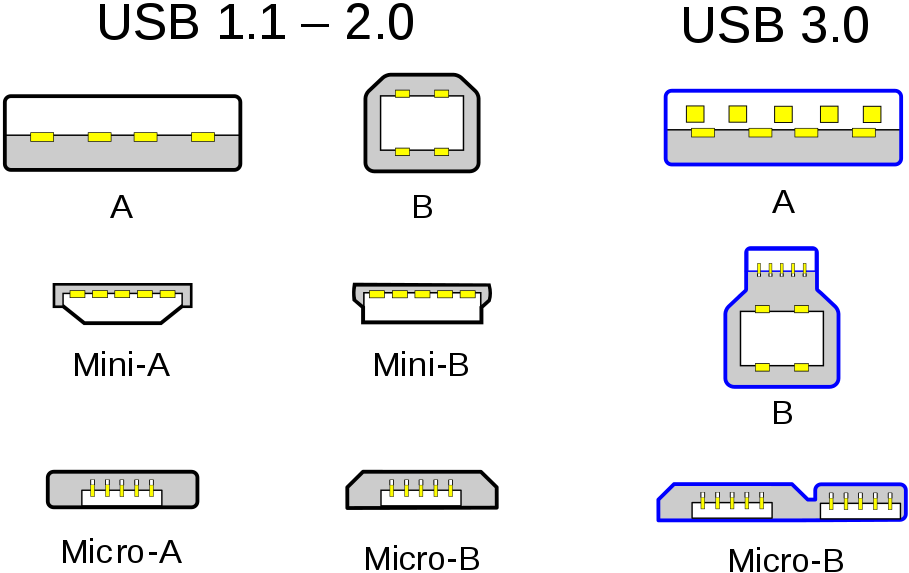
\includegraphics[width=0.4\linewidth]{usb.png}
    \vspace{-5pt}
    \captionof{figure}{Distintos conectores USB. Fuente: \href{https://es.wikipedia.org/wiki/Universal_Serial_Bus}{wikipedia}}
\end{center}

\vspace{-10pt}
Para la nueva especificación USB-C trajo consigo un nuevo conector que es reversible (se puede conectar en ambas direcciones), con idea de reemplazar todos los conectores anteriores. La idea es que ambos dispositivos (anfitrión y huésped) se hace uso del mismo conector y el cable que los una llegue a ser universal, teniendo en cuenta la especificación que utilice.

\vspace{-15pt}
\begin{center}
    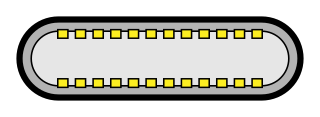
\includegraphics[width=0.25\linewidth]{usb-c.png}
    \vspace{-10pt}
    \captionof{figure}{USB-C. Fuente: \href{https://es.wikipedia.org/wiki/USB-C}{wikipedia}}
\end{center}

Las \hyperlink{placa_base}{placas bases} tienen varios conectores USB typo-A soldados para poder realizar conexiones, pero también tiene conexiones en la placa para poder tener más USB (por ejemplo, gracias a los que vienen en la caja).

Estos conectores externos tienen un cable que se conectan a unos pines en la placa base, que dependiendo del protocolo, tendrán una forma u otra (por eso es importante ver el manual de la placa base).

\vspace{-10pt}
\begin{center}
    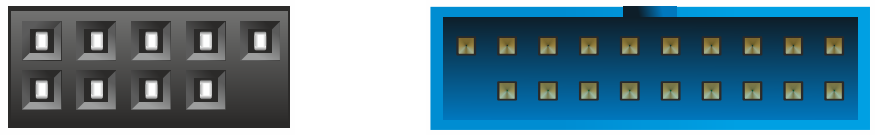
\includegraphics[width=0.35\linewidth]{usb_placa_base.png}
    \vspace{-10pt}
    \captionof{figure}{Conector USB-2 y USB-3 en placa base (pines)}
\end{center}


\subsubsection{Conexiones de red}

Para que nuestro ordenador se pueda conectar a una red, las placas base ya tienen incorporado al menos un conector para ello.

\begin{minipage}{0.15\linewidth}
    
\includegraphics[width=\linewidth]{rj45.png}
\end{minipage}
\hfill
\begin{minipage}{0.8\linewidth}
    El conector \textbf{RJ-45} es el utilizado en redes de ordenadores que contiene cuatro pares de cables de cobre para realizar la transmisión de datos a través del protocolo \textbf{ethernet}, que veremos más adelante.
\end{minipage}


\vspace{12pt}
\begin{minipage}{0.15\linewidth}
    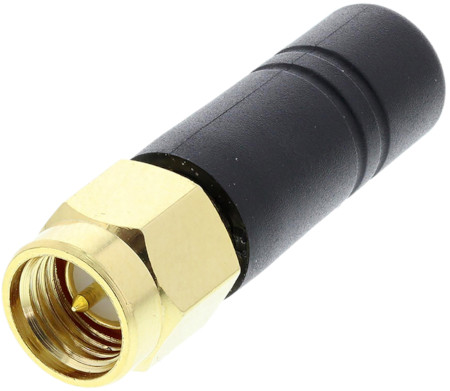
\includegraphics[width=\linewidth]{sma.jpg}
\end{minipage}
\hfill
\begin{minipage}{0.8\linewidth}
    El conector \textbf{SMA} se utiliza en algunos tipos de antenas WiFi desmontables que nos podemos encontrar en algunos routers, placas base, tarjetas PCI... Es un conector enroscable y fácilmente desmontable.
\end{minipage}


\vspace{12pt}
\begin{minipage}{0.15\linewidth}
    
\includegraphics[width=\linewidth]{ps2.png}
\end{minipage}
\hfill
\begin{minipage}{0.8\linewidth}
    \textbf{PS\/2} era el conector utilizado para realizar la conexión de teclados y ratones antes de la llegada del USB. Normalmente venía con dos colores, violeta para el teclado y verde para el ratón, ya que aunque el conector era el mismo, el teclado requiere en ambos lados un colector abierto para permitir la comunicación bidireccional.
\end{minipage}

\vspace{12pt}
\begin{minipage}{0.15\linewidth}
    
\includegraphics[width=\linewidth]{jack.png}
\end{minipage}
\hfill
\begin{minipage}{0.8\linewidth}
    El \textbf{jack} de 3,5mm es el conector más utilizado para audio analógico desde hace muchos años en el ordenador, a pesar de que su aparición (en distinto tamaño) es del año 1878. Hoy en día las placas base tienen distintos conectores para introducir estos jacks dependiendo de si es para altavoces, micrófono, sonido envolvente...
\end{minipage}


\vspace{12pt}
\begin{minipage}{0.15\linewidth}
    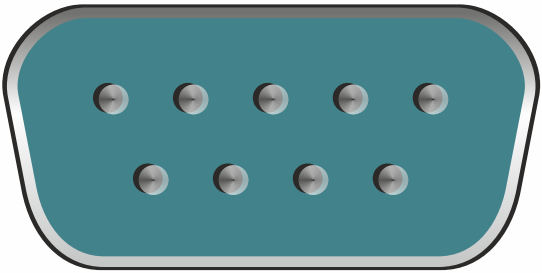
\includegraphics[width=\linewidth]{serie.png}
\end{minipage}
\hfill
\begin{minipage}{0.8\linewidth}
    El conector \textbf{RS232} (también conocido como “puerto serie”), es un interfaz que permite el intercambio de datos binarios entre dos equipos. Originalmente para mandar información a un terminal de datos, y posteriormente muy utilizado en switches. Aunque hoy en día las placas base no tienen el conector externo, suelen tener los pines de conexión para añadir un adaptador.
\end{minipage}


Desde que los ordenadores se hicieron populares en la década de los 80 hasta ahora ha habido muchos otros tipos de conectores que han llegado a los ordenadores de consumo personal.

También ha habido otros muchos tipos de conectores que se han quedado en el ámbito más profesional (\href{https://es.wikipedia.org/wiki/Transceptor_SFP}{transceiver SFP}, conectores \href{https://es.wikipedia.org/wiki/Serial_Attached_SCSI}{SAS} para discos duros, ...) por lo que es imposible abarcarlos a todos.


\subsubsection{Conector, protocolo y cables: errores frecuentes}

Hemos visto distintos conectores que durante años su forma física no ha variado, buscando ser retrocompatible con versiones anteriores, pero que la transmisión de velocidad sí se ha ido incrementando a lo largo de los años.

Algunos ejemplos:

\begin{itemize}
    \item PCI
    \item USB
    \item SATA
    \item HDMI
    \item DisplayPort
\end{itemize}

Es por eso que es importante entender y comprender que la forma del conector hoy en día no nos tiene por qué indicar la velocidad de transmisión máxima que acepta el dispositivo conectado, y por eso deberemos ir a las especificaciones técnicas de la placa base o el dispositivo concreto.

Por otro lado, \textbf{con los cables sucede lo mismo}. Debemos confirmar y asegurar que los cables que utilizamos van a ser capaz de transmitir la velocidad máxima que tanto dispositivo como placa base aceptan.


\errorbox{\textbf{Es importante conocer las especificaciones técnicas de cada componente y cable que usemos, para no realizar ningún cuello de botella.}}
\vspace{10pt}

\subsection{Caja del ordenador}
La caja del ordenador, o chasis, es la estructura metálica donde se introducen (de manera ordenada, y anclando mediante tornillos) los distintos componentes que hemos visto hasta ahora.

Existen distintos tipos de caja, normalmente variando el tamaño, por lo que es importante adecuar la caja a los componentes que queramos albergar dentro.

\warnbox{\textbf{Cuidado con coger una caja demasiado pequeña y que luego la placa base, o la anchura de la tarjeta gráfica no entre}}
\vspace{10pt}

\begin{center}
    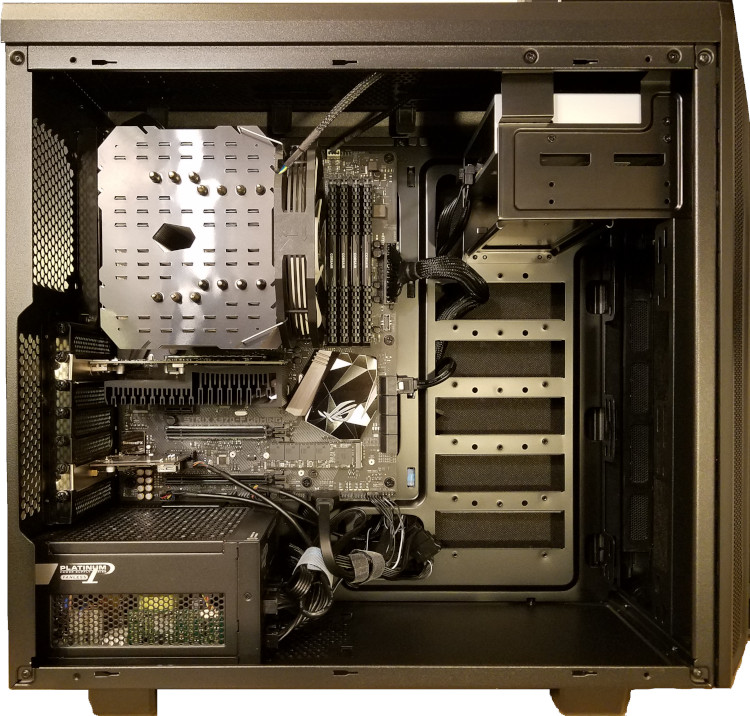
\includegraphics[width=0.75\linewidth]{caja.jpg}
    \vspace{-10pt}
    \captionof{figure}{Caja con ordenador instalado. Fuente: \href{https://en.wikipedia.org/wiki/Computer_case}{wikipedia}}
\end{center}


Los servidores cuentan con unas cajas de tamaño estandarizados en altura, denominado “\href{https://es.wikipedia.org/wiki/Unidad_rack}{Unidad de Rack}” (\textit{rack unit} en inglés, o simplemente “U”), cuya unidad equivale a 44.45 milímetros. De esta manera los servidores contarán con una altura fijada para poder ser instalados en un \href{https://es.wikipedia.org/wiki/Bastidor_de_19_pulgadas}{bastidor \textit{rack}}.

\begin{center}
    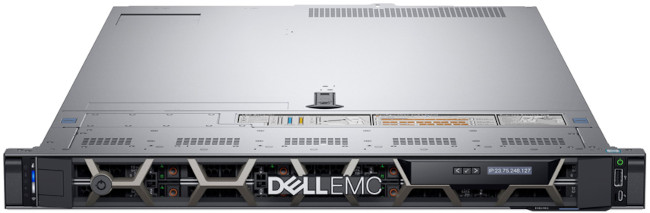
\includegraphics[width=0.75\linewidth]{servidor.jpg}
    \vspace{-10pt}
    \captionof{figure}{Servidor Dell 1U de altura}
\end{center}


\section{Arranque de un ordenador}

Una vez el hardware está instalado, es momento de entender cómo funciona el sistema de arranque de nuestro ordenador hasta llegar al Sistema Operativo.

Toda la secuencia de arranque se puede dividir en distintas etapas que vamos a ver a continuación:

\begin{enumerate}
    \item Se acciona el botón de encendido del equipo (o arranca el equipo tras un reinicio).
    \item Se carga la BIOS/UEFI y se comienza a ejecutar.
    \item Se realiza el \textit{Power-On Self-Test} (POST), que es una secuencia que comprueba el estado de los componentes hardware. En caso de que algún componente no parezca estar correcto, la placa base emitirá sonidos. \textbf{Si este paso falla, no continuará el proceso}.

    \infobox{Es habitual que si algún componente falla, la placa base emita uno o varios tonos (si tiene un speaker/altavoz) de distinta duración}

    \begin{itemize}
        \item Comprobación del procesador
        \item Se comprueba el estado de la RAM y la cantidad instalada
        \item Comprueba el estado de la memoria de vídeo.
        \item Inicializa los sistemas de acceso a dispositivos de almacenamiento (IDE, Serial-ATA, NVMe...).
    \end{itemize}

    \item La BIOS/UEFI comprueba el número de discos duros existentes. Se comprueba la tabla de particiones del disco duro indicado como primario para el arranque.
    \item Se ejecuta el gestor de arranque de la tabla de particiones marcada como arrancable.
    \item El gestor de arranque prepara todo lo que necesita el Sistema Operativo para funcionar, lo carga y le transfiere la ejecución a él.
\end{enumerate}

\chapter{Discos duros: particionado y sistemas de ficheros}
Anteriormente hemos visto que los \hyperlink{dispositivos_almacenamiento}{sistemas de almacenamiento} (más conocidos como discos duros) son dispositivos que pueden ser de distintos tipos, capacidades, tamaños...

A la hora de usar un disco duro en nuestro Sistema Operativo, tenemos que tener en cuenta al menos dos cosas:

\begin{itemize}
    \item \textbf{Tipo de particionado}.
    \item \textbf{Sistema de ficheros}.
\end{itemize}

Dependiendo del Sistema Operativo, y el modo que elijamos durante la instalación, nos dará más opciones o menos a la hora de elegir, modificar o personalizar algunas de estas opciones.

Para tomar las decisiones correctas, deberíamos conocer, al menos, los siguientes detalles:

\begin{itemize}
    \item Número de discos duros instalados en el equipo.
    \item El tipo de cada uno (mecánico, SSD, NVMe...).
    \item Tamaño de los mismos.
    \item Función que va a realizar el equipo.
\end{itemize}

De esta manera, podremos realizar un análisis previo de cómo queremos realizar la instalación.


\section{Particionado MBR y GPT }
Los discos duros se dividen en lo que se llaman particiones. Es una manera de realizar divisiones lógicas del espacio, que actúan de forma independiente entre sí.

\textbf{El símil del particionado de disco duro es un armario}: tenemos una cantidad de hueco posible, que decidimos “particionar” añadiendo estanterías tanto horizontales como verticales, donde almacenar distintos tipos de ropa, de manera independiente, en cada uno de esos compartimentos.

A la hora de crear la tabla de particiones de un disco duro podemos elegir entre los siguientes tipos:

\begin{itemize}
    \item \textbf{MBR}: De \textit{Master Boot Record}, o también conocido como \textbf{tabla de particiones DOS}.
    \item \textbf{GPT}: De \textit{GUID Partition Table}, propuesta por la especificación EFI, más moderna que la anterior.
\end{itemize}

En la siguiente tabla se pueden identificar algunas de las diferencias más destacadas entre ambos sistemas:

\begin{yukitblrcol}{XXX}
    & MBR & GPT\\
    Tamaño máximo de partición & 2 TB & 18 Exabytes \\
    Nº de particiones primarias & 4 & Ilimitado

     (Windows reconoce 128)\\
    Tabla de particiones& Al inicio & Al inicio y al final (backup) \\
    ID de la partición & Se almacena en la partición & Identificador único de GUID\\
    Soporte de arranque múltiple & Débil & Las entradas del gestor de arranque están en una partición separada  \\
\end{yukitblrcol}

Para comprobar cuál es el sistema de particiones de nuestro disco duro lo podemos hacer desde:
\begin{itemize}
    \item En \textbf{Windows}: Desde el administrador de discos duros.
    \item En \textbf{GNU/Linux}: Con GParted, fdisk, ...
\end{itemize}

A continuación se pueden ver capturas de pantalla de distintos discos en un equipo Windows.


    \begin{minipage}{0.45\linewidth}
        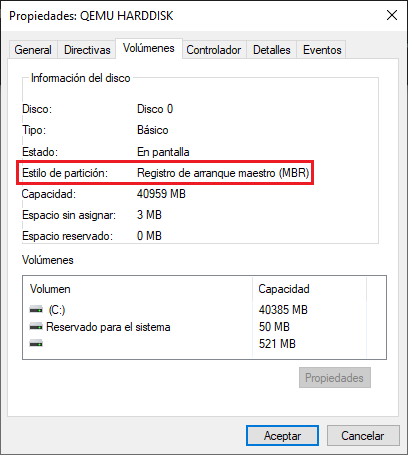
\includegraphics[frame,width=\linewidth]{hdd_mbr.png}
    \end{minipage}
    \hfill
    \begin{minipage}{0.45\linewidth}
        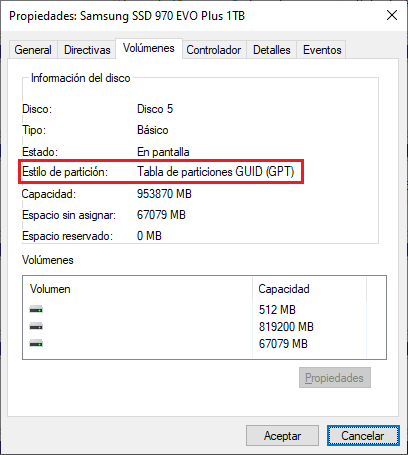
\includegraphics[frame,width=\linewidth]{hdd_gpt.png}
    \end{minipage}


\section{Sistemas de ficheros}
Los sistemas de ficheros controlan cómo se almacenan y recuperan los datos. Sin un sistema de archivos, los datos colocados en un medio de almacenamiento serían un gran cuerpo de datos sin manera de saber dónde termina un dato y comienza el siguiente.

Un fichero (o archivo) es una secuencia de bytes almacenado en un dispositivo que es identificado por un nombre. Los ficheros pueden ser almacenados en directorios, y estos a su vez en otros directorios.

Por lo tanto, un sistema de ficheros nos proporciona una “\textit{vista lógica}” de cómo se almacenan los datos.

Las funciones principales de los sistemas de ficheros son:

\begin{itemize}
    \item Asignar espacio a los archivos.
    \item Administrar el espacio libre.
    \item Provee una API a los programas para crear, borrar, modificar y cerrar los ficheros.
    \item Permite gestionar el acceso a los ficheros (permisos de ficheros).
    \item Optimizar el rendimiento de acceso.
\end{itemize}



    \graphicspath{{../../../temas_comunes/particionado_sistemas_ficheros_raid/img}}
    \chapter{Particionado y sistemas de ficheros}
Anteriormente hemos visto que los \hyperlink{dispositivos_almacenamiento}{sistemas de almacenamiento} (más conocidos como discos duros) son dispositivos que pueden ser de distintos tipos, capacidades, tamaños...

A la hora de usar un disco duro en nuestro Sistema Operativo, tenemos que tener en cuenta al menos dos cosas:

\begin{itemize}
    \item \textbf{Tipo de particionado}.
    \item \textbf{Sistema de ficheros}.
\end{itemize}

Dependiendo del Sistema Operativo, y el modo que elijamos durante la instalación, nos dará más opciones o menos a la hora de elegir, modificar o personalizar algunas de estas opciones.

Para tomar las decisiones correctas, deberíamos conocer, al menos, los siguientes detalles:

\begin{itemize}
    \item Número de discos duros instalados en el equipo.
    \item El tipo de cada uno (mecánico, SSD, NVMe...).
    \item Tamaño de los mismos.
    \item Función que va a realizar el equipo.
\end{itemize}

De esta manera, podremos realizar un análisis previo de cómo queremos realizar la instalación.


\section{Particionado MBR y GPT }
Los discos duros se dividen en lo que se llaman particiones. Es una manera de realizar divisiones lógicas del espacio, que actúan de forma independiente entre sí.

\textbf{El símil del particionado de disco duro es un armario}: tenemos una cantidad de hueco posible, que decidimos “particionar” añadiendo estanterías tanto horizontales como verticales, donde almacenar distintos tipos de ropa, de manera independiente, en cada uno de esos compartimentos.

A la hora de crear la tabla de particiones de un disco duro podemos elegir entre los siguientes tipos:

\begin{itemize}
    \item \textbf{MBR}: De \textit{Master Boot Record}, o también conocido como \textbf{tabla de particiones DOS}.
    \item \textbf{GPT}: De \textit{GUID Partition Table}, propuesta por la especificación EFI, más moderna que la anterior.
\end{itemize}

En la siguiente tabla se pueden identificar algunas de las diferencias más destacadas entre ambos sistemas:

\begin{yukitblrcol}{XXX}
    & MBR & GPT\\
    Tamaño máximo de partición & 2 TB & 18 Exabytes \\
    Nº de particiones primarias & 4 & Ilimitado

    (Windows reconoce 128)\\
    Tabla de particiones& Al inicio & Al inicio y al final (backup) \\
    ID de la partición & Se almacena en la partición & Identificador único de GUID\\
    Soporte de arranque múltiple & Débil & Las entradas del gestor de arranque están en una partición separada  \\
\end{yukitblrcol}

Para comprobar cuál es el sistema de particiones de nuestro disco duro lo podemos hacer desde:
\begin{itemize}
    \item En \textbf{Windows}: Desde el administrador de discos duros.
    \item En \textbf{GNU/Linux}: Con GParted, fdisk, ...
\end{itemize}

A continuación se pueden ver capturas de pantalla de distintos discos en un equipo Windows.


\begin{minipage}{0.45\linewidth}
    \includegraphics[frame,width=\linewidth]{hdd_mbr.png}
\end{minipage}
\hfill
\begin{minipage}{0.45\linewidth}
    \includegraphics[frame,width=\linewidth]{hdd_gpt.png}
\end{minipage}


\section{RAID}

RAID (en inglés \textit{redundant array of independent disks}) es un grupo o matriz redundante de discos independientes que hace referencia a un sistema para crear una unidad de almacenamiento lógica utilizando varias unidades de almacenamiento. De esta manera, \textbf{el sistema operativo sólo ve un único almacenamiento lógico, que “por detrás” utiliza varios}.

Dependiendo del tipo de grupo creado, los datos se distribuirán o se replicarán entre las unidades que forman el grupo.

A la hora de crear un sistema RAID, podemos hacerlo de dos maneras:
\begin{itemize}
    \item \textbf{RAID por hardware}: Existe un hardware especializado que se encarga de realizar las operaciones del sistema RAID, así como de crearlo, gestionarlo, hacer las operaciones de paridad necesarias... Podemos diferenciar dos sub-tipos:

    \begin{itemize}
        \item \textbf{Placa Base}: Algunas placas base tienen un controlador especializado que se encarga de la creación del RAID, que se puede gestionar desde el sistema UEFI.
        \item \textbf{Tarjeta controladora especializada}: Este sistema es el \textbf{más profesional}. Los discos duros en lugar de ir conectados a la placa base, se conectan a esta tarjeta (normalmente a través de unos cables especiales que se conectan por SATA al disco duro y mediante conectores especiales a la tarjeta). Hay veces que cuentan con una batería propia (para controlar la escritura en caso de que el servidor se quede sin alimentación) y con un menú propio de configuración.
    \end{itemize}

    \item \textbf{RAID por software}: El Sistema Operativo se encarga de crear y gestionar el sistema RAID. En caso de necesitar realizar paridad, la CPU se encargará de ello, quitando recursos a otros procesos.
\end{itemize}

Tal como se puede ver en la \href{https://es.wikipedia.org/wiki/RAID}{Wikipedia}, existen distintos tipos de RAID, que también pueden combinarse entre sí, pero a continuación se explicarán los más estándares.

\subsection{RAID 0}

\begin{minipage}{0.63\linewidth}
    \setlength{\parskip}{1.2em}

    Un sistema RAID 0 distribuye los datos de manera equitativa entre dos o más discos, sin hacer uso de información de paridad. RAID 0 \textbf{no habilita redundancia}, por lo que \textbf{si uno de los discos duros del sistema se estropea, se perderán todos los datos}.

    \textbf{Espacio total = sumatorio del espacio de los discos.}

    Con este sistema se puede conseguir una mayor velocidad de escritura, ya que los datos se escriben de manera simultánea en todos los discos.


\end{minipage}
\hfill
\begin{minipage}{0.28\linewidth}
    \includegraphics[width=\linewidth]{Raid0.png}
    \vspace{-30pt}
    \captionof{figure}{Fuente: \href{https://commons.wikimedia.org/wiki/File\:Raid0.png}{Wikipedia}}
\end{minipage}

\errorbox{
    \begin{center}
        \textbf{No se aconseja utilizar RAID 0 en sistemas con datos importantes.}
    \end{center}
}

\vspace{10pt}
\subsection{RAID 1}
\begin{minipage}{0.63\linewidth}
    \setlength{\parskip}{1.2em}
El RAID 1, también conocido como RAID espejo, crea una copia exacta de los datos en dos o más sistemas de almacenamiento.

Resulta útil cuando queremos tener seguridad a la hora de preservar los datos a pesar de no aprovechar la capacidad total del conjunto de los discos. \textbf{Si uno de los discos falla, los datos no se pierden}.

\textbf{El RAID 1 sólo puede ser tan grande como el más pequeño de los discos.}

No se mejora el rendimiento en escritura, pero en la lectura el tiempo se reduce al poder usar varios discos de forma simultánea.
\end{minipage}
\hfill
\begin{minipage}{0.28\linewidth}
\includegraphics[width=\linewidth]{Raid1.png}
\vspace{-30pt}
\captionof{figure}{Fuente: \href{https://commons.wikimedia.org/wiki/File\:Raid1.png}{Wikipedia}}
\end{minipage}


\subsection{RAID 5}

RAID 5 es una división de los datos a nivel de bloques que distribuye la información entre el conjunto de discos que lo forman, y añadiendo \textbf{paridad}. La paridad se utiliza para poder corregir errores o generar los datos en caso de pérdida de uno de los discos.

Para crear un sistema RAID 5 se necesitan al menos 3 discos duros, quedando uno de ellos “inutilizado” en lo que se refiere a guardar información.

\textbf{El volumen total = (n-1)*tamaño de disco más pequeña}, donde “n” es el número de discos que forman el RAID 5. Si tenemos 3 discos de 2TB, el tamaño total será = (3-1)*2TB = 4TB.

En caso de rotura de un disco duro, los datos se mantienen, pero el sistema RAID 5 no soportaría la rotura de un segundo disco duro. Es por ello que cuando sucede esto, hay que sustituir el disco dañado para que se regeneren los datos en el nuevo disco duro, gracias al sistema de paridad.

\begin{center}
    \includegraphics[width=0.5\linewidth]{Raid5.png}
    \vspace{-15pt}
    \captionof{figure}{Fuente: \href{https://commons.wikimedia.org/wiki/File\:Raid5.png}{Wikipedia}}
\end{center}

\subsubsection{Discos spare/reserva}

Existen variantes de RAID 5, y algunas controladoras hardware también implementan, la posibilidad de tener discos denominados “\textbf{\textit{hot spare}}”, o \textbf{de reserva}.

Estos discos están conectados (a la controladora, o la placa base) pero sin estar dentro del grupo RAID. Entrarán a formar parte del grupo en el momento en el sistema detecte que uno de los discos pertenecientes al grupo está fallando, y por tanto el sistema RAID esté degradado.

De esta manera, al entrar en el grupo, el RAID comenzará a arreglarse de manera automática sin tener que esperar a que el administrador de sistemas se entere de que ha habido algún error.


\section{Sistemas de ficheros}
\textbf{Los sistemas de ficheros controlan cómo se almacenan y recuperan los datos}. Sin un sistema de archivos, los datos colocados en un medio de almacenamiento serían un gran cuerpo de datos sin manera de saber dónde termina un dato y comienza el siguiente.

\infobox{\textbf{Un sistema de ficheros nos proporciona una “\textit{vista lógica}” de cómo se almacenan los datos.}}

Las funciones principales de los sistemas de ficheros son:

\begin{itemize}
    \item Asignar espacio a los archivos.
    \item Administrar el espacio libre (reorganizándolo en caso necesario).
    \item Provee una API a los programas para crear, borrar, modificar y cerrar los ficheros.
    \item Permite gestionar el acceso a los ficheros (permisos de ficheros).
    \item Optimizar el rendimiento de acceso.
\end{itemize}


\subsection{Ficheros}
Un fichero (o archivo) es una secuencia de bytes almacenado en un dispositivo que \textbf{es identificado por un nombre y normalmente una extensión}. Los ficheros pueden ser almacenados en directorios, y estos a su vez en otros directorios.

En inglés sí existe distinción entre \textbf{\textit{file}} y \textbf{\textit{archive}} siendo la diferencia:

\begin{itemize}
    \item \textbf{File}: Es un conjunto de información que se almacena de manera conjunta. Cómo se almacena esa información depende de cómo se ha diseñado el programa que lee y/o escribe esa información.
    \item \textbf{Archive}: Un archivo es un conjunto de ficheros almacenados junto con \textit{\textbf{metadata}} (datos que aportan información sobre datos). El ejemplo más claro puede ser un archivo comprimido, archivos que permiten distribuir programas, ...
\end{itemize}

Los ficheros cuentan con un nombre para que los podamos identificar. Dependiendo del sistema de ficheros puede ser:
\begin{itemize}
    \item \textbf{Case sensitive}: O sensible a mayúsculas/minúsculas. Esto quiere decir que “hola.txt” y “HOla.txt” son dos ficheros distintos.
    \item \textbf{Case insensitive}: O insensible a mayúsculas/minúsculas. No puede haber dos ficheros con las mismas letras en el mismo orden, aunque sean mayúsculas y minúsculas. “hola.txt” y “HOla.txt” no pueden convivir en el mismo directorio.
\end{itemize}

Los ficheros suelen contar con una \textbf{extensión}, que va después del nombre seguido de un punto, y normalmente suele ser de 3 letras para la mayoría de casos. Estas extensiones sirven para conocer el tipo de fichero a simple vista, pero no determina el contenido del fichero.

\warnbox{\textbf{La extensión no determina el tipo de fichero que es. Si renombramos un fichero con una extensión, el contenido del fichero sigue siendo el mismo}}

Un pequeño listado de  \href{https://en.wikipedia.org/wiki/List_of_filename_extensions}{extensiones}  habituales que podemos identificar:

\begin{itemize}
    \item \textbf{Documentos de texto y ofimáticos}: .txt, .doc, .docx, .xls, .xlsx, .ppt, .pptx, .odt, .odp, .ods, .pdf ...
    \item \textbf{Ficheros multimedia, imagen, audio, vídeo}: .png, .jpg, .jpeg, .tiff, .ps, .bmp, .svg, .gif, .mp3, .mp4, .avi, .mpg, .mpeg, .mkv, ...
    \item \textbf{Archivos comprimidos}: .zip, .bz2, .gz, .gzip, .7z, .rar, .r00, ...
    \item \textbf{Archivos de programación}: .c, .java, .class, .py, .php, .rb, .pl, .sh, ...
\end{itemize}

En los sistemas Windows las extensiones están ocultas en el explorador de archivos, por lo que para un usuario sin conocimientos, no existen.



\subsection{Sistemas de ficheros más utilizados}

Existen \href{https://en.wikipedia.org/wiki/List_of_file_systems}{muchos sistemas de ficheros}, y cada Sistema Operativo suele utilizar uno por defecto, que es el que está optimizado para sus funciones. Eso no quita que pueda hacer uso de otros sistemas de ficheros en otros dispositivos.

\infobox{\textbf{Los Sistemas Operativos utilizan un sistema de ficheros predeterminado, pero suelen poder acceder a dispositivos que hagan uso de otros}}

A continuación se expone una tabla con los sistemas de ficheros predeterminados de distintos Sistemas Operativos y los sistemas de fichero que pueden leer por defecto:

\begin{yukitblr}{X X X}
    Sistema Operativo & Sistema de Ficheros & Puede leer \\
    \textbf{DOS, Windows 95} & FAT16 &  \\
    \textbf{Windows 95 OSR2\linebreak Windows 98} & FAT16, FAT32 &  \\
    \textbf{ Windows NT, 2000, XP,...  \linebreak Windows 10, Windows 11 } & NTFS (varias versiones)  & FAT16, FAT32  \\
    \textbf{Windows Server > 2012, Windows 11 } & NTFS, ReFS  & FAT16, FAT32, NTFS \\
    \textbf{GNU/LInux} & Ext4, ReiserFS & La gran mayoría \\
    \textbf{MacOS} & HFS+, APFS & FAT16, FAT32 \\
\end{yukitblr}

Existen programas y drivers para permitir que los sistemas operativos puedan leer otros sistemas de ficheros que no pueden en origen. \textbf{A veces pueden tener limitaciones (en la escritura, permisos, ...)}.

En la \href{https://en.wikipedia.org/wiki/Comparison_of_file_systems}{Wikipedia} existe un listado con distintas características de un gran listado de sistemas de ficheros. A continuación parte de esa información:

\begin{yukitblrcol}{X[2]XXXXX}
    & FAT 32 & NTFS & ReFS & EXT-4 & APFS \\
    Nombre de fichero max. & 8.3 (255) & 255 & 255 & 255 & 255 \\
    Volumen max. & 16TB & 16TB & 1YB & 1 EB & ? \\
    Tamaño max. fichero & 4GB & 16TB & 16EB & 16TB & 8 EB \\
    Permisos & No & Si & Si & Si & Si\\
    Compresión & No & Si & No & No & Si\\
    Cifrado & No & Si & No/Si & Si & Si\\
\end{yukitblrcol}

Debido a que los sistemas de ficheros van adquiriendo características nuevas, es posible que algunas no estuviesen en las primeras versiones y fueran añadidas a \textit{posteriori}.


\section{Jerarquía de directorios}
A la hora de almacenar la información en un sistema de ficheros, se hace siguiendo una jerarquía de directorios. Esta jerarquía de directorios es creada por el sistema operativo durante la instalación y en ella se almacenan los ficheros necesarios para el sistema.

Posteriormente la jerarquía puede ser expandida para guardar información de usuarios, o para que programas y servicios puedan guardar y utilizar información. \textbf{La estructura inicial debe ser conservada y no se debe modificar si no estamos seguros de lo que hacemos}.

\errorbox{\textbf{Los directorios y ficheros creados durante la instalación del Sistema Operativo forman parte de una estructura “inmutable”. Si se modifican/mueven es posible que el sistema deje de funcionar. ¡CUIDADO!}}

\subsection{Sistemas Windows}
Microsoft comenzó a utilizar el sistema denominado “\href{https://es.wikipedia.org/wiki/Letra_de_unidad}{letra de unidad}” con el lanzamiento de MS-DOS, aunque no fueron los primeros en utilizarlos.

Este sistema utiliza una letra del alfabeto para identificar los volúmenes o unidades lógicas de sistemas de almacenamiento.

Tanto en MS-DOS como en Windows, se denomina de la siguiente manera:

\begin{itemize}
    \item \textbf{A:\textbackslash} Es la unidad de \hyperlink{disquete}{disquete}.
    \item \textbf{B:\textbackslash} Reservada para la segunda unidad de disquete.
    \item \textbf{C:\textbackslash} Partición o disco duro principal. Donde se instala el sistema operativo y los programas.
    \item \textbf{D:\textbackslash} Reservado para el CD-ROM/DVD-ROM.
    \item \textbf{E:\textbackslash} hasta \textbf{Z:} para otro discos duros, particiones, CD-ROMs/DVD-ROM, sistemas extraíbles de almacenamiento...
\end{itemize}

También se puede utilizar este sistema para carpetas compartidas por red, aunque no es necesario.

\subsection{GNU/Linux}
En los sistemas operativos GNU/Linux (aunque también sucede en las variantes UNIX como FreeBSD y MacOS) la jerarquía comienza en un único punto representado con “\textbf{/}” denominado \textbf{directorio raiz} o “barra”.

El \href{https://es.wikipedia.org/wiki/Filesystem_Hierarchy_Standard}{\textbf{\textit{Filesystem Hierarchy Standard}} (FHS)} es la referencia para conocer dónde se deben almacenar los ficheros dentro de la jerarquía, siendo algunos de los directorios más conocidos. Más adelante hablaremos de ello.

    \graphicspath{{img/si/}}
    \chapter{Software}
El software es el elemento lógico que forma parte del ordenador, todo aquello que es “intangible”. Es el \textbf{conjunto de programas y datos} que permiten manejar el \hyperlink{hardware}{hardware}, controlando y coordinando su funcionamiento para que realice las tareas deseadas.

% para no copiar un trozo que ya tenemos en el fichero 1_introduccion.tex

\ExecuteMetaData[1_introduccion]{tipossoftware}

%
%    \section{Tipos de Software}
%    \subsection{firmware,sistema y aplicaciones}
%
%    \subsection{Licencias de Software}
%
%    \section{Sistemas Operativos}


    \part{Sistemas de comunicación y redes}
    \graphicspath{{../../../temas_comunes/sistemas_de_comunicacion/img}}
    \chapter{Introducción a los sistemas de comunicación}

Desde el principio de los tiempos, el ser humano se ha comunicado con sus congéneres de distintas maneras: comenzó a través de la voz (se cree que hace unos 100.000 años), con algún tipo de protolenguaje, para posteriormente comenzar a utilizar sistemas de comunicaciones permanentes (la escritura).

Por todos es conocido la evolución histórica de distintos sistemas de comunicación, entre los que podemos destacar (\href{https://es.wikipedia.org/wiki/Anexo:Cronolog%C3%ADa_de_las_tecnolog%C3%ADas_de_la_comunicaci%C3%B3n}{referencia}):
\begin{itemize}
    \item \textbf{Pinturas rupestres}: Realizadas en cuevas o rocas en las que se pueden observar escenas de caza, distintos animales, grabado de manos, figuras humanas... Algunas de las pinturas encontradas cuentan con más de 50.000 años. Tenemos un ejemplo cercano en las \href{https://es.wikipedia.org/wiki/Cueva_de_Santimami\%C3\%B1e}{cuevas de Santimamiñe} en donde tenemos pinturas datadas entre 14.000 y 9.000 años a. C.

    \item \textbf{Escritura cuneiforme}: Es uno de los primeros sistemas de escritura realizados, y se utilizaban tablillas de arcilla húmeda en las que se grababa mediante un tallo vegetal. Con este sistema se han datado tablas anteriores al 3.200 a.C. y en distintos idiomas.

    \item \textbf{Escritura jeroglífica y el papiro}: En el antiguo Egipto se crea la escritura mediante signos que comienza por escribirse en paredes para posteriormente inventar el papiro (cuya datación más antigua es del 2.500 a.C.) y de esta manera se comienza a tener un sistema de comunicación fácilmente manejable e intercambiable.

    \item \textbf{Uso de palomas mensajeras}: El uso de palomas mensajeras para el envío de comunicaciones data de la época anterior a 1.500 a.C. y se ha estado utilizando hasta este siglo en algunos países durante desastres naturales.

    \item \textbf{Imprenta}: El primer documento impreso data de china del año 868, pero la imprenta moderna la creó en 1440, más o menos, \href{https://es.wikipedia.org/wiki/Johannes_Gutenberg}{Johannes Gutemberg}. Gracias a la imprenta la creación de documentos escritos se realizaba de manera más rápida y esto permitió que la expansión del conocimiento escrito se acelerase.

    \item \textbf{Telégrafo}: A partir de mediados del siglo XVIII y durante el inicio del siglo XIX hubo bastantes avances en las investigaciones del electromagnetismo y de esta manera se comenzó a investigar cómo usarlo para el envío de señales. En 1837 Samuel Morse patenta el \href{https://es.wikipedia.org/wiki/Tel%C3%A9grafo#Historia_del_tel%C3%A9grafo}{telégrafo}. En \textbf{1858} se une Irlanda y Terranova mediante el \textbf{primer cable trasatlántico}.

    \item \textbf{Teléfono}: Como evolución al telégrafo, que sólo permitía el envío de señales, nace el teléfono de la mano de \href{https://es.wikipedia.org/wiki/Antonio_Meucci}{Antonio Meucci} (aunque normalmente se le atribuye el invento a \href{https://es.wikipedia.org/wiki/Alexander_Graham_Bell}{Alexander Graham Bell}). En 1860 realizó una demostración pública transmitiendo voz a una considerable distancia.
\end{itemize}

Tal como podemos ver, ha habido distintos sistemas de comunicación utilizados durante siglos para el envío y recepción de información.

\section{Comunicación de la información}

Tal como hemos visto, los sistemas de comunicación de la información no es algo nuevo, ¿pero qué necesidades tiene un sistema de comunicación?

\begin{itemize}
    \item \textbf{Emisor}: Es el origen y la fuente de la información que se pretende comunicar.
    \item \textbf{Receptor}: Es el destinatario, el que va a recibir la información.
    \item \textbf{Mensaje}: Es la información que queremos transmitir entre el emisor y el recepetor.
    \item \textbf{Código}: Es el conjunto de reglas utilizadas a la hora de representar el mensaje. El emisor y receptor deben utilizar el mismo código para que la comnunicación sea correcta.
    \item \textbf{Canal}: Es el medio físico por el que se va a enviar el mensaje.
    \item \textbf{Señal}: Es el componente físico por el que se envía la información.
\end{itemize}

Para entender de mejor manera un sistema de comunicación y los componentes que lo forman, vamos a poner dos ejemplos:

\subsubsection*{Ejemplo 1: Comunicación oral}

\begin{wrapfigure}{r}{0.25\linewidth}
    \centering
    \vspace{-35pt}
    \includegraphics[width=\linewidth]{comunicacion-1.png}
    \vspace{-30pt}
\end{wrapfigure}
En este ejemplo vemos que hay dos personas, las cuales se han identificado cada una de ellas como “Emisor” y “Receptor”, y así de esta manera conocemos quién es el origen y quién el destino de la comunicación.

En este caso, el \textbf{mensaje} es “Hola”, haciendo uso del \textbf{código} conocido como “castellano”. La \textbf{señal} que se va a utilizar es la voz, ya que están hablando y el \textbf{canal} por el que se envía el mensaje es el aire.

Es un ejemplo sencillo que utilizamos cada día.

\subsubsection*{Ejemplo 2: Comunicación escrita por mensajería}

\begin{wrapfigure}{r}{0.25\linewidth}
    \centering
    \vspace{-35pt}
    \includegraphics[width=\linewidth]{comunicacion-2.png}
    \vspace{-30pt}
\end{wrapfigure}
AL igual que en el ejemplo anterior, vemos que hay dos personas, las cuales se han identificado cada una de ellas como “Emisor” y “Receptor” pero que en este caso se van a comunicar haciendo uso de un teléfono móvil, tal como hacemos en nuestro día a día a través de una aplicación de mensajería o red social.

Teniendo en cuenta esto, en este ejemplo realmente existen dos sistemas de comunicación que están mezclados y uno está por encima del otro:

\begin{itemize}
    \item \textbf{Entre personas}: Similar al ejemplo anterior, el emisor y el receptor se están comunicando, con el mensaje compuesto por tres \href{https://es.wikipedia.org/wiki/Emoji}{emojis} que representan estar riendo. El \textbf{código} es el idioma que estén utilizando, el \textbf{canal} sería el programa utilizado y la \textbf{señal} podríamos decir que es el móvil.

    \item \textbf{Entre dispositivos}: En este caso, el emisor y receptor es el móvil de cada usuario. El mensaje es el mismo, pero convertido a un sistema digital (como el \hyperlink{binario}{binario}). El \textbf{canal} en este caso sería el aire y la \textbf{señal} es la utilizada por el móvil, por ejemplo el 5G.
\end{itemize}

Tal como se puede ver en este caso, una comunicación puede depender a su vez de otro sistema de comunicación.

\subsection{Esquema de la comunicación}
Para simplificar cómo se realiza la comunicación, podemos utilizar el siguiente esquema:

\begin{center}
    \vspace{-10pt}
    \includegraphics[width=0.6\linewidth]{comunicacion-esquema.png}
    \vspace{-10pt}
\end{center}


    \graphicspath{{../../../temas_comunes/introduccion_a_redes/img}}
    \chapter{Redes de comunicación}
En el ámbito informático una red de comunicaciones es representada como una red de ordenadores para poder compartir información, recursos u ofrecer servicio (ya sea al usuario o a otros ordenadores).

Las redes de ordenadores son un conjunto de equipos hardware que están conectados entre sí, mediante cables o de manera inalámbrica, y que a través de un software especializado envían y reciben impulsos eléctricos (u ondas electromagnética) para el transporte de datos.


\section{Breve historia de las redes}
A continuación una breve cronología mostrando los hitos más importantes dentro de las redes de comunicaciones, en lo que a ordenadores se refiere (\href{https://en.wikipedia.org/wiki/Computer_network}{Referencia}).

\begin{description}
    \item[\textasciitilde 1950]
    En la década de los 50 se desarrollan los circuitos integrados. Esto hará que en el futuro los ordenadores cada vez se vayan haciendo más pequeños.

    Las redes de ordenadores comienzan a aparecer en las bases militares americanas, en principio para sistemas de radares.

    \item[\char`\~ 1960]
    Se realiza una conexión entre dos mainframes en EEUU para el sistema de reservas aéreas comerciales.

    El \href{https://es.wikipedia.org/wiki/Instituto_de_Tecnolog%C3%ADa_de_Massachusetts}{MIT} utiliza un ordenador para enrutar y mantener conexiones telefónicas.

    En 1966, aparece un paper (artículo científico) describiendo las WAN.

    En 1969 ARPANET (red de ordenadores creadas por el Departamento de Defensa de Estados Unidos) cuenta con 4 nodos (a 50kbit/s de velocidad).

    \item[\char`\~ 1970]
    En 1972 se hace la primera demostración pública de ARPANET.

    A comienzos de la década (1973) se crea Ethernet en la compañía Xerox Parc.

    A finales de la década Xerox intenta hacer que Ethernet se convierta en un estándar de conexión para terminar con las competencias (token ring, …).

    \begin{center}
        \vspace{-10pt}
        \includegraphics[frame,width=0.9\linewidth]{Arpanet_logical_map_march_1977.png}
        \vspace{-5pt}
        \captionof{figure}{Mapa lógico de ARPANET, marzo de 1977. Origen: \href{https://es.wikipedia.org/wiki/ARPANET\#/media/Archivo:Arpanet_logical_map,_march_1977.png}{ Wikipedia}}\vspace{-13pt}
    \end{center}

    \item[\char`\~ 1980]
    Los ordenadores personales empiezan a generalizarse.

    Aparece el protocolo para enviar y recibir e-mails (SMTP).

    El protocolo TCP/IP se convierte en el utilizado por ARPANET (1983) y es declarado como su estándar para las comunicaciones.

    Aparece el servicio DNS.

    Se crea el modelo de referencia OSI.

    Aparece el primer gusano por la red (Morris worm, 1988). Se estima que infectó al 10\% de los ordenadores conectados a la red.

    Se crea el protocolo BGP.

    El protocolo Ethernet evoluciona y permite conexiones a 10Mbit/s.


    \item[\char`\~ 1990]
    Tim Berners-Lee desarrolla el código para WWW y crea el primer servidor web (1991).

    Se puede decir que aquí es cuando nace la Internet que conocemos actualmente.

    En 1995 Ethernet permite conexiones a 100Mbit/s

    Se establece un control para los nombres de dominio (posteriormente lo asumirá ICANN).

    Aparece Amazon, ebay, Craiglist, IMDB, hotmail, google, yahoo, ...

    Aparece el protocolo IPv6 (1998).

    Aparece el protocolo wifi 802.11b.

    \item[\char`\~ 2000]
    Crisis de las “.com”.

    Internet se generaliza.

    Empiezan a permitirse más TLDs, que no corresponden sólo a países.

    Ethernet permite conexiones a 1Gbit/s

    \item[\char`\~ 2010]
    Ethernet permite conexiones a 400Gbit/s (2018).

    \href{https://en.wikipedia.org/wiki/Starlink}{Starlink} comienza a desplegar su constelación de satélites para dar cobertura en todo el planeta.


\end{description}

\section{Tipos de redes}
A la hora de diferenciar las redes de ordenadores podemos diferenciarlas por distintos conceptos:

\begin{itemize}
    \item Por el medio de transmisión utilizado.
    \item Por la dirección de los datos.
    \item Por el alcance.
    \item Por el grado de acceso.
    \item Por la topología.
    \item ...
\end{itemize}

\subsection{Por el medio de transmisión utilizado}
Más adelante veremos distintos \hyperlink{sistemas_transmision}{sistemas de transmisión}, pero para ir diferenciando podemos crear dos grandes grupos teniendo en cuenta el medio utilizado:

\begin{itemize}
    \item \textbf{Guiados}: Es decir, a través de cables que se encargarn de realizar la transmisión de la señal desde un punto de origen al punto de destino.

    \item \textbf{No guiados}: Se hace uso de algún sistema inalámbrico (mediante antenas) para realizar la transmisión de los datos.
\end{itemize}


\subsection{Por la dirección de los datos}
Si tenemos en cuenta la dirección de los datos en la transmisión, podemos diferenciarlos como:

\begin{itemize}
    \item \textbf{Simplex}: la comunicación sólo se realiza en un único sentido, por lo que sólo es necesario un único canal de transmisión.

    \item \textbf{Half-duplex}: se permite la comunicación en ambos sentidos, pero no de manera simultánea, por lo que emisor y receptor se reparten el tiempo de emisión. Por ejemplo, el \textit{\textbf{walkie-talkie}}.

    \item \textbf{Duplex}: O también conocido como \textit{full-duplex}, permite la comunicación en ambas direcciones y de manera simultánea. Por ejemplo, el \textbf{teléfono}. Para ello es necesario tener una de estas dos opciones:
    \begin{itemize}
        \item Dos canales Half-duplex: uno para cada dirección de la comunicación.
        \item Un único canal por el que se envía la comunicación, pero para ello es necesario algún sistema de multiplexación (como puede ser usar frecuencias separadas).
    \end{itemize}
\end{itemize}


\subsection{Por alcance}
Teniendo en cuenta el alcance al que llegan las redes, podríamos realizar la siguiente distinción:

\subsubsection{Red de área personal (PAN)}
Del inglés \textit{Personal Area Network}, es aquella en la que interactúan distintos dispositivos de muy corto alcance, limitado al área de una persona.

El ejemplo más habitual hoy día sería la comunicación mediante tecnología inalámbrica por Bluetooth en la comunicación entre ordenador, móvil y dispositivos como un \textit{smartwatch}.


\subsubsection{Red de área local (LAN)}
Del inglés \textit{Local Area Network}, es una red que puede abarcar un cierto área de tamaño como una casa, una oficina, un colegio, una universidad...

El ejemplo de una oficina sería una red en la que existen distintos ordenadores, que pueden comunicarse entre sí o compartir información con un servidor ya sea a través de una red cableada o también inalámbrica.

\subsubsection{Red de área metropolitana (MAN)}
Del inglés \textit{Metropolitan Area Network}, y como su nombre indica, el área es mayor y suele abarcar una ciudad para ofrecer los servicios necesarios en la misma.

En este caso también puede ser de manera cableada (normalmente haciendo uso de tecnología más rápida como es la fibra óptica) y también de manera inalámbrica.

Dentro de los servicios que pertenecerían a una MAN podemos poner como ejemplos:
\begin{itemize}
    \item Despliegue de zonas WIFI gratuito en la ciudad.
    \item Comunicación entre sistemas de información (paradas de autobuses, marquesinas, ...).
    \item Sistemas de video-vigilancia municipal.
\end{itemize}

Algunos de estos servicios que están en una MAN pueden ser públicos (como el WIFI) o de acceso restringido (sistemas de seguridad).

\subsubsection{Red de área amplia (WAN)}
Del inglés \textit{Wide Area Network}, es una red que abarca grandes extensiones geográficas y normalmente construidas por grandes empresas o proveedores de internet (ISP, \textit{Internet Service Provider}).


\subsection{Por el grado de acceso}
Teniendo en cuenta quién puede acceder a la red, podríamos definir dos tipos de redes:

\begin{itemize}
    \item \textbf{Red privada}: es una red que sólo ciertas personas pueden acceder y que no normalmente no es accesible desde otras redes. El ejemplo más sencillo es la red que tenemos en casa.
    \item \textbf{Red pública}: es una red a la que puede acceder cualquier persona y que interconecta otras redes sin importar su situación geográfica. Internet es una red pública.
\end{itemize}

%\subsection{Por la topología}
%La topología de una red indica cómo están interconectados los nodos de la misma y el camino que pueden realizar los datos cuando viajan por esa red. En resumen: \textbf{es el diseño de la red}.

%TODO: completar información

    \graphicspath{{../../../temas_comunes/sistemas_de_comunicacion/img}}
    \chapter{Arquitectura en capas}
Un sistema de comunicación se pueden diferenciar en distintos niveles en los que cada uno realiza una función independiente, pero que a su vez interactúan con los niveles limítrofes.

\begin{center}
    \vspace{-10pt}
    \includegraphics[width=0.4\linewidth]{comunicacion-esquema.png}
    \vspace{-10pt}
\end{center}

Este ejemplo es un modelo simplificado de comunicación, y dentro de una arquitectura de red de ordenadores pueden existir más capas en las que pueden existir distintas funciones extra que no aparecen en este esquema.

\section{Origen}

Al comienzo de las redes de ordenadores cada empresa creaba su propio sistema de comunicación creando su propio hardware y software, lo que hacía imposible la interconexión entre equipamiento de distintas empresas.

Estos sistemas de comunicación constan de unas reglas que los nodos deben conocer para poder comunicarse entre sí, y a ese conjunto de reglas se les denomina \textbf{protocolo de comunicación}.


Para que eso hoy en día no suceda ya que las redes están definidas en varios estándares, como veremos más adelante.

\infobox{Un \textbf{estándar} es un conjunto de normas que pueden abarcar distintos niveles (tanto software como hardware) que ha sido aceptado, o creado, por la gran mayoría de las empresas del sector para poder realizar la interconexión e intercomunicación entre sí.}


\section{Ventajas de la división en capas}

La división en capas nos permite:
\begin{itemize}
    \item Dividir el proceso de comunicación en procesos más pequeños.

    \item Aislar las funciones de cada capa. De esta manera, en caso de realizar modificaciones en la misma, no afecta al resto de capas.

    \item Ocultar la implementación al resto de capas. Siguiendo con el punto anterior, una capa utilizará los servicios de su capa inferior sin saber cómo realiza sus funciones.

    \item Cada capa puede constar de distintos estándares, facilitando la interconexión de distintas tecnologías
\end{itemize}

Una arquitectura de red en capas se implementa por medio de distintos protocolos, formando una familia de protocolos para facilitar la comunicación de distintos sistemas y equipos en la red.

\infobox{Una arquitectura en capas nos permite que cada capa actúe de manera independiente y que incluya sus propios protocolos. Cada capa dispone de una serie de servicios que ofrece a su capa limítrofe superior.}

Desde el comienzo de las redes de ordenadores han existido distintas familias de protocolos, y se puede considerar que hubo una \href{https://en.wikipedia.org/wiki/Protocol_Wars}{guerra de protocolos durante las décadas de 1970 a 1990}. Empresas, organizaciones y países se posicionaban sobre cuál sería el mejor protocolo de comunicaciones y el que saldría ganador para el uso a nivel internacional.

Por destacar algunos protocolos que ya no se usan:

\begin{itemize}
    \item \textbf{\href{https://en.wikipedia.org/wiki/Systems_Network_Architecture}{SNA}} creado en 1974 por IBM.
    \item \textbf{\href{https://en.wikipedia.org/wiki/NetBIOS_Frames}{NetBEUI}} de Microsoft. Que evolucionó a NetBIOS sobre TCP/IP que hoy día se usa en Windows Server.
    \item \textbf{\href{https://en.wikipedia.org/wiki/IPX/SPX}{IPX/SPX}} de Novell.
\end{itemize}

\section{Modelo de referencia OSI}
El modelo de interconexión de sistemas abiertos, conocido como “modelo \textbf{OSI}” (\textit{\textbf{O}pen \textbf{S}ystems \textbf{I}nterconnection} en inglés) es un \textbf{modelo de referencia (teórico)} que busca estandarizar las funciones de comunicación para un sistema informático siendo agnóstico a la tecnología utilizada para realizar la implementación y a los protocolos utilizados en cada capa.

El diseño comenzó en 1977 tratando de terminar con la \href{https://en.wikipedia.org/wiki/Protocol_Wars}{guerra de protocolos} comentada previamente, y la Organización Internacional de Estandarización (\textit{International Organization for Standardization}, o \textbf{ISO} en inglés)  terminó por definir el estándar ISO-7498 en 1984.


\subsection{Capas en el modelo OSI}
El modelo OSI está compuesto por siete capas numeradas del 1 al 7 siendo la 1 la más baja y haciendo referencia a la parte física de la red.


%TODO: modificar tabla?
\begin{yukitblr}{X X X[3,l]}
    Capa & Nombre de la unidad de datos & Función \\

    7ª - Aplicación & Datos
    & APIs de alto nivel, como compartir recursos y acceso remoto a archivos. \\

    6ª - Presentación & Datos
    & Traducción de datos entre un servicio de red y una aplicación, que incluye la codificación de caracteres, la compresión de datos y el cifrado y descifrado de datos.
    \\

    5ª - Sesión & Datos
    & Manejo de sesiones de comunicación, por ejemplo el continuo intercambio de información en forma de múltiples transmisiones hacia ambos lados entre dos nodos.
    \\

    4ª - Transporte & Segmento, Datagrama
    & Transmisión de segmentos de datos confiable entre puntos de red, incluyendo la segmentación, el acknowledgement y la multiplexación.
    \\

    3ª - Red & Paquete
    & Estructura y manejo de una red multinodo. Incluye el direccionamiento, el ruteo y el control de tráfico.
    \\

    2ª - Enlace de datos & Trama
    & Transmisión de datos confiable entre dos nodos conectados mediante una capa física.
    \\

    1ª - Física & Bit, Baudios
    & Transmisión y recepción de flujos de bits sin procesar por un medio físico.
    \\
\end{yukitblr}


\section{Pila de protocolos TCP/IP}

Durante el surgimiento de las redes de comunicaciones entre ordenadores cada fabricante creaba su propio estándar, lo que hacía que la comunicación entre ellos no fuese posible. En 1974  \href{https://en.wikipedia.org/wiki/Vint_Cerf}{Vint Cerf} and \href{https://en.wikipedia.org/wiki/Bob_Kahn}{Bob Kahn} describen un protocolo para compartir recursos usando envío de paquetes a través de una red de comunicación. Es el comienzo del protocolo \textbf{TCP}.

En 1984 fue el protocolo elegido por parte del Departamento de Defensa de Estados Unidos, y poco tiempo después se convirtió en el estándar de facto de la comunicación de red que posteriormente dio lugar a Internet.

Tal como se puede ver, la pila de protocolos TCP/IP es funcional, al contrario que ocurre con el modelo OSI que sólo es teórico.

La pila TCP/IP cuenta con cuatro capas:

\begin{yukitblr}{X X X[3,l]}
    Capa & Protocolos conocidos & Función \\

    4ª - Aplicación
    & HTTP, FTP, POP, SMTP, ...
    & Es la capa más cercana al usuario, utilizada por las aplicaciones a la hora de enviar datos
    \\

    3ª - Transporte
    & TCP, UDP
    & Estructura y manejo de una red multinodo. Incluye el direccionamiento, el ruteo y el control de tráfico.
    \\

    2ª - Red
    & IPv4, IPv6
    & Transmisión de datos confiable entre dos nodos conectados mediante una capa física.
    \\

    1ª - enlace
    & Ethernet, IEEE 802, 802.11 (wifi)
    & Es una mezcla de las capas 1 y 2 del modelo OSI.
    \\
\end{yukitblr}


\subsection{Protocolo TCP}

El objetivo del protocolo TCP es crear conexiones dentro de una red de datos compuesta por redes de ordenadores para intercambiar datos. La ventaja es que el protocolo busca garantizar que los datos son entregados a su destino sin errores y en el mismo orden en el que se transmitieron.

Por otro lado, también proporciona un mecanismo para distinguir distintas aplicaciones dentro de una misma máquina, a través del concepto de \textbf{puerto}.

Hoy día TCP es el protocolo más utilizado dentro de las aplicaciones que hacen uso de comunicación en red. Por ejemplo, los protocolos HTTP, SMTP, SSH, FTP... hacen uso de TCP como como protocolo de transporte (\textbf{capa 4 del modelo OSI}).


\subsubsection{Establecer comunicación}
A la hora de establecer una comunicación usando el protocolo TCP lo habitual es que en el lado del \textbf{servidor (el receptor de la comunicación)} exista un servicio que esté “\textit{escuchando}” en un puerto previamente levantado (por ejemplo, un servidor web que escucha en el \textbf{puerto 80 y 443}).

El cliente comenzará la comunicación enviando un paquete \textbf{SYN} a la IP del servidor y al puerto con el que se quiere comunicar, a lo que si todo ha ido bien, el servidor responderá con la respuesta \textbf{SYN/ACK}.
\begin{wrapfigure}{r}{0.35\linewidth}
    \hfill
    \vspace{-30pt}
    \includegraphics[width=0.9\linewidth]{tcp-handshake.png}
    \vspace{-10pt}
\end{wrapfigure}

Finalmente, el cliente debería responderle al servidor con un ACK, completando así la \textbf{negociación en tres pasos} (SYN, SYN/ACK y ACK) y la fase de establecimiento de conexión.

De esta manera, comenzará la transferencia de datos, a lo que se le añade una serie de mecanismos que determinan la fiabilidad y robustez del protocolo. Entre ellos están incluidos:


\begin{itemize}
    \item Uso del número de secuencia para ordenar los segmentos TCP recibidos y detectar paquetes duplicados.
    \item \textit{Checksums} para detectar errores.
    \item Indicación por parte del receptor que ha recibido los paquetes para detectar pérdidas.
    \item Temporizadores para detectar retrasos o necesidad de reenvío de información.
\end{itemize}


\subsubsection{Cierre de la comunicación}
\begin{wrapfigure}{r}{0.35\linewidth}
    \hfill
    \includegraphics[width=0.9\linewidth]{tcp-fin.png}
    \vspace{-10pt}
\end{wrapfigure}
La fase de finalización de la conexión utiliza una negociación en cuatro pasos (four-way handshake), terminando la conexión desde cada lado independientemente.

Cuando uno de los dos extremos de la conexión desea parar su "mitad" de conexión transmite un segmento con el flag FIN en 1, que el otro interlocutor asentirá con un ACK. Por tanto, una desconexión típica requiere un par de segmentos FIN y ACK desde cada lado de la conexión.

Una conexión puede estar "medio abierta" en el caso de que uno de los lados la finalice pero el otro no. El lado que ha dado por finalizada la conexión no puede enviar más datos pero la otra parte si podrá.



\subsubsection{Puertos TCP}
TCP usa el concepto de número de puerto para identificar a las aplicaciones emisoras y receptoras. Cada lado de la conexión TCP tiene asociado un número de puerto (de 16 bits sin signo, con lo que existen 65536 puertos posibles) asignado por la aplicación emisora o receptora.

Los \textbf{puertos bien conocidos} son asignados por la Internet Assigned Numbers Authority (IANA), van del 0 al 1023 y son usados normalmente por el sistema o por procesos con privilegios. Algunos ejemplos son: FTP (21), SSH (22), Telnet (23), SMTP (25) y HTTP (80).

Los \textbf{puertos registrados} son normalmente empleados por las aplicaciones de usuario de forma temporal cuando conectan con los servidores, pero también pueden representar servicios que hayan sido registrados por un tercero (rango de puertos registrados: 1024 al 49151).

Los \textbf{puertos dinámicos/privados} también pueden ser usados por las aplicaciones de usuario, pero este caso es menos común. Los puertos dinámicos/privados no tienen significado fuera de la conexión TCP en la que fueron usados (rango de puertos dinámicos/privados: 49152 al 65535.

    \graphicspath{{../../../temas_comunes/direccionamiento_ipv4/img}}
    \chapter{Direccionamiento IPv4}

La \textbf{dirección IP} es el identificador (que debe ser único) de un dispositivo dentro de una red. Los dispositivos pertenecientes a la misma red podrán comunicarse entre sí mediante dicha dirección IP. Todas las características que conforman esta IP están explicados en el \textbf{protocolo IP} (\href{https://es.wikipedia.org/wiki/Protocolo_de_internet}{Internet Protocol}).

Debido a que en el origen de la creación del protocolo IPv4 no se pensaba que llegase a haber tantos dispositivos conectados a internet, el límite que se puso para el número de posibles direcciones está llegando a su fin. Es por ello que ya existe un nuevo protocolo, \textbf{IPv6} desde hace tiempo, que sustituirá a IPv4 en un futuro, pero para ello debe de realizarse una transición que no termina de finalizar, aunque ya es posible hacer uso de ello.

El direccionamiento IP proporciona un mecanismo para la asignación de identificadores a cada dispositivo conectado a una red. Antes de dar información más técnica, exponemos los principales conceptos:

\begin{itemize}
    \item Una dirección IP es un conjunto de bits (que formarán 4 números decimales), que sirve para identificar de forma única a un dispositivo dentro de la red.
    \item La asignación de dicha IP se puede realizar de dos maneras:
    \begin{itemize}
        \item \textbf{Estática}: El administrador del dispositivo deberá configurar la dirección de manera manual teniendo en cuenta los parámetros necesarios que se ajusten a la red a la que se quiere conectar.
        \item \textbf{Dinámica}: Una vez el dispositivo se conecte de manera física a la red (por cable, o en caso de ser de manera inalámbrica, realizando la conexión  al SSID e introduciendo la contraseña) habrá un servicio (\textbf{DHCP}) que le otorgará una IP.
    \end{itemize}
\end{itemize}

El protocolo IPv4 permite la existencia de dos tipos de direcciones:

\begin{itemize}
    \item \textbf{Direcciones públicas}: Son las utilizadas en Internet. Cualquier dispositivo que se conecte de manera directa a Internet debe tener un direccionamiento público. Existe la organización \href{https://es.wikipedia.org/wiki/Corporaci%C3%B3n_de_Internet_para_la_Asignaci%C3%B3n_de_Nombres_y_N%C3%BAmeros}{ICANN} que se encarga de repartir estos direccionamientos entre los proveedores de internet.

    \item \textbf{Direcciones privadas}: Son direcciones asignadas a dispositivos que se encuentran dentro de una red que no tiene visibilidad desde Internet. Los dispositivos que tienen este tipo de direccionamiento privado no pueden acceder a internet a través de su IP, por lo que debe de haber un dispositivo que le oculte su IP privada y se la “cambie” por una IP del rango público (el \textbf{router} realizando \textbf{NAT}, lo veremos más adelante).
\end{itemize}

\section{Formato de una dirección IPv4}

Como ya se ha comentado, una IP es un conjunto de bits, concretamente 32, que normalmente son representados en 4 grupos de 8 bits pasados a decimal, que es lo que normalmente estamos acostumbrados a ver:

\begin{itemize}
    \item Dirección IP en formato de 32 bits:
    \begin{center}
        \texttt{11000000101010000000000101100100}
    \end{center}
    \item IP en formato de bits, separados:
    \begin{center}
        \texttt{11000000  10101000  00000001  01100100}
    \end{center}
    \item Dirección IP en formato decimal:
    \begin{center}
        \texttt{192\space\space\space\space\space\space .168\space\space\space\space\space\space\space.1\space\space\space\space\space\space\space .100}
    \end{center}
\end{itemize}

Al tener 32 bits, se realizan 4 grupos de 8 bits, por lo que obtendremos \textbf{$2^{8}$} posibles combinaciones en cada grupo. Por lo que nos lleva a poder representar cualquier número desde 0 (\texttt{00000000}) hasta 255 (\texttt{11111111}) en cada bloque.



\section{Máscara de red}

Una dirección IP no sólo contiene la dirección única de un dispositivo, sino que también contiene la red a la que pertenece dicho dispositivo. Esto nos lleva a ver que una IP pertenece a una jerarquía, ya que pertenece a una red “superior”. A simple vista no podemos saber a qué red pertenece una IP, pero el formato es el siguiente:

\begin{center}
    \includegraphics[width=0.8\linewidth]{mascara_de_red.png}
\end{center}

Dependiendo del número de bits que sea “n”, el número “m” variará a la par hasta que ambos sumen los 32 bits que debe de tener una dirección IP. Aquí es donde entra en juego la \textbf{máscara de red}.

La máscara de red es un número binario de 32 bits que nos permitirá conocer qué número es “n” y “m” en una dirección IP, para así obtener el prefijo de la red y conocer cuántos dispositivos puede llegar a existir en la red.

Al igual que la IP, \textbf{una máscara de red son 32 bits} que contendrán a la izquierda “n” unos y a la derecha “m” ceros.

\warnbox{\textbf{En la máscara de red a la izquierda irán los \texttt{1} y a la derecha los \texttt{0}. ¡Nunca se mezclan!}}

Por ejemplo:
\begin{itemize}
    \item \textbf{IP decimal}:\hspace{22pt} \texttt{192.168.1.100}
    \item \textbf{IP binario}:\hspace{25pt} \texttt{11000000101010000000000101100100}
    \item \textbf{Máscara de red}: \texttt{11111111111111110000000000000000}
\end{itemize}

Si contamos el número de unos que tenemos en el lado izquierdo de la máscara de red veremos que tenemos 16, por lo que los primeros 16 bits de la IP serán los que nos digan a qué red pertenece esa IP. En este caso, y para favorecer el visionado, realizamos una separación de los bits:

\begin{itemize}
    \item \textbf{IP binario}:\hspace{25pt} \texttt{11000000\space\space10101000\space\space00000001\space\space01100100}
    \item \textbf{Máscara de red}: \texttt{11111111\space\space11111111\space\space00000000\space\space00000000}
\end{itemize}

Con esto obtenemos:
\begin{itemize}
    \item \textbf{Prefijo de la red}: \texttt{192.168}
    \item \textbf{Identificador del dispositivo:} \texttt{1.100}
\end{itemize}

Si observamos, la máscara de red, al ser 32 bits, también se puede escribir en formato decimal, aplicando al igual que antes, la creación de 4 grupos de 8 bits. En el ejemplo anterior \textbf{la máscara sería: \texttt{255.255.0.0}} .

Existe un tercer método para escribir la máscara de red:  “\textbf{/n}”, donde “\textbf{n}” es un número indicando el número de \textbf{unos} (y por tanto, los bits que identifican el prefijo de la red) que tiene la máscara de red. En nuestro caso, la máscara también se puede escribir como \textbf{/16}, ya que es el número de unos que tiene nuestra máscara.

\section{Nombre de la red, broadcast y dispositivos}

De una máscara y una IP podemos obtener más información. Para conocer el \textbf{número de posibles IPs que puede llegar a haber en esa red} tendremos que realizar el cálculo de $2^{m}$, donde “m” es el número de ceros que tiene la máscara.

En nuestro ejemplo es $2^{16} = 65536$ posibles IPs. \textbf{De estas IPs existen dos IPs especiales}:

\begin{itemize}
    \item \textbf{Nombre de la red}: El nombre de la red sirve para identificar y diferenciar las distintas redes que pueden llegar a existir.

    Es muy importante nombrarlas de manera correcta ya que nos dará la información necesaria para conocer el prefijo de la red y el número posible de dispositivos que puede haber.

    Para crear el nombre de la red lo haremos usando el prefijo de la red y el resto de bits ponerlos a 0. En nuestro ejemplo:

    \begin{center}
        \textbf{\texttt{11000000  10101000  00000000  00000000 = 192.168.0.0}}
    \end{center}

    \textbf{Al nombre de la red siempre se le debe añadir la máscara}, por lo que quedaría:  \texttt{\textbf{192.168.0.0 /16}}

    \errorbox{\textbf{Si no se pone la máscara de red, podría ser una IP suelta de cualquier red}}

    \item \textbf{Broadcast}: Sirve para poder mandar un mensaje a todos los dispositivos de la red. Para formar esta dirección usamos el prefijo de la red y el resto de bits ponerlos a 1, por lo que en nuestro ejemplo quedaría:

    \begin{center}
        \textbf{\texttt{11000000  10101000  11111111  11111111 = 192.168.255.255}}
    \end{center}
\end{itemize}

Teniendo esto en cuenta, al total de posibles IPs de una red tendremos que restarle 2 para darnos el número total de dispositivos que podremos tener en una red:


\infobox{
\begin{center}
\textbf{Para saber el número de posibles IPs de una red: }

        {\Large $2^{m} - 2$}

\textbf{siendo “m” el número de “\texttt{0}” de la máscara}
\end{center}
}

En nuestro ejemplo vemos que “m” es 16 (porque en la máscara tenemos 16 ceros), y sabemos que tenemos 2 IPs especiales (\textbf{el nombre de la red} y \textbf{el broadcast}) que tendremos que restar para tener el número total de dispositivos (tablets, ordenadores, móviles conectados) que podrá llegar a tener esa red:  $2^{16} - 2 = 65534$ posibles dispositivos. El rango de estos dispositivos será desde la IP \texttt{\textbf{192.168.1.1}} hasta \texttt{\textbf{192.168.255.254}}.


\section{Bloques de IPs reservadas}
Dentro de todas las posibles IPs y redes que podemos llegar a crear, existen unos bloque que están \href{https://en.wikipedia.org/wiki/Reserved_IP_addresses}{reservados} por unas razones u otras:

\begin{itemize}
    \item \textbf{Redes públicas}: son todas las IPs que no entran en los siguientes bloques, y por tanto, son las utilizadas públicamente en Internet.

    \item \textbf{Redes privadas}: Son redes que sólo pueden existir en el ámbito privado y no se podrá configurar de cara internet.

    \item \textbf{Reservado}: Existen varios bloques que están reservados por diversas razones, de los cuales veremos los ejemplos más característicos.
\end{itemize}

Es importante conocer los bloques reservados para no cometer errores a la hora de crear redes. El listado completo se puede encontrar en la \href{https://es.wikipedia.org/wiki/IPv4#Direcciones_de_uso_especial}{Wikipedia}.


\subsection{Bloque reservado: 127.0.0.0 /8}

La primera dirección de este bloque, 127.0.0.1, es el utilizado como bucle local (o \textbf{loobpack}). Este conjunto de IPs hacen referencia al propio equipo en el que nos encontramos y se suelen utilizar para hacer pruebas locales.


\subsection{Redes privadas}

Una red privada es una red de computadoras que usa el espacio de direcciones IP especificadas más adelante. A los equipos o terminales se les puede asignar direcciones de este espacio cuando deban comunicarse con otros terminales dentro de la red interna/privada.

Los nombre de las redes privadas son:

\begin{itemize}
    \item \textbf{\texttt{10.0.0.0 /8}}
    \item \textbf{\texttt{172.16.0.0 /12}}
    \item \textbf{\texttt{192.168.0.0 /16}}
\end{itemize}

Estas redes privadas no son siempre utilizadas con su máxima máscara posible, ya que en la mayoría de los casos se estarían desperdiciando IPs.

El utilizar en nuestra red privada un rango que no sea uno de estos tres signfica que estamos yendo en contra de las reglas establecidas por la ICANN.

\subsection{Reservado para despliegues Carrier Grade NAT}

En abril de 2012, el IANA asignó el rango \textbf{100.64.0.0/10} para uso en escenarios de \href{https://es.wikipedia.org/wiki/Carrier_Grade_NAT}{Carrier Grade NAT} en el \href{https://www.rfc-editor.org/rfc/rfc6598}{RFC 6598}.

Este bloque de direcciones no debe ser usado en redes privadas o en la Internet pública: ha sido pensado para operaciones de uso interno en redes de teleoperadores. El tamaño del bloque de direcciones (aproximadamente 4 millones de direcciones, $2^{22}$) ha sido seleccionado para ser suficientemente grande para acomodar todos los dispositivos de acceso de un solo operador en un punto de presencia en una red de área metropolitana como la de Tokio (Fuente: \href{https://es.wikipedia.org/wiki/Carrier_Grade_NAT}{Wikipedia}).

\subsection{Bloque reservado para el futuro}
Existe el bloque completo \textbf{\texttt{240.0.0.0 /8}} cuyas IPs están reservadas para pruebas y para el futuro. Es conocido como la “clase E”.


\subsection{Otros bloques}
Como ya se ha comentado, en la \href{https://en.wikipedia.org/wiki/Reserved_IP_addresses}{Wikipedia} se pueden encontrar todos los bloques reservados que no son públicos y la razón por las que han sido reservados.


\section{Clases de IP}
Durante el inicio de la expansión de internet y la creación de redes se crearon clases que nos indican el número de subredes que deberían existir, la máscara y más información que \textbf{hoy en día se considera obsoleta}.

\begin{itemize}
    \item \textbf{Clase A}: se asigna el primer octeto para identificar la red, reservando los tres últimos octetos (24 bits) para que sean asignados a los hosts, de modo que la cantidad máxima de hosts es $2^{24} - 2$ . El bit más significativo (el de más a la izquierda) empieza por 0.

    \item \textbf{Clase B}: se asignan los dos primeros octetos para identificar la red, reservando los dos octetos finales (16 bits) para que sean asignados a los hosts. Los primeros bits más significativos son 10:

    \item \textbf{Clase C}: se asignan los tres primeros octetos para identificar la red, reservando el octeto final (8 bits) para que sea asignado a los hosts, de modo que la cantidad máxima de hosts por cada red es $2^{8} - 2$ . Los primeros bits más significativos son 110
\end{itemize}

\section{Configurar IPv4}

Una vez sabemos cómo funciona IPv4, es el momento de aplicarlo en el sistema operativo en el que nos encontremos.

\subsection{IPv4 en Windows}

Por defecto, la configuración de red en Windows solicita una dirección IP de manera automática cuando el cable está conectado en el interfaz de red.

Para conocer la configuración actual de la red podemos utilizar el comando \commandbox{ipconfig} desde el terminal de windows. Si le pasamos el parámetro “/all” ( \commandbox{ipconfig /all} ), el resultado del comando nos dará más información, como es la configuración del DNS, la dirección física (MAC), ...

\begin{center}
    \includegraphics[width=0.8\linewidth]{ipconfig.png}
\end{center}


Si queremos realizar la modificación de la red, podremos hacer uso del icono de red que está al lado de la hora. Para ver toda la configuración, podemos ir al “Panel de Control → Redes e Internet → \textbf{Configuración de Red e Internet}”. Elegimos “Protocolo de Internet versión 4”, le damos a “Propiedades” y podremos realizar la configuración siguiente:


\begin{center}
    \includegraphics[width=0.7\linewidth]{cambiar_ip_windows.png}
\end{center}


En la imagen se puede ver la configuración realizadA:
\begin{itemize}
    \item \textbf{Dirección IP}: La dirección IP que queremos que tenga el equipo.
    \item \textbf{Máscara de subred}: La máscara de red a la que pertenece la IP que hemos configurado.
    \item \textbf{Puerta de enlace predeterminada}: Para que el equipo tenga conexión con otras redes, debemos indicar qué IP tiene el \textbf{\textit{gatway}}.
\end{itemize}

Aparte, podemos realizar la configuración del servidor DNS primario y secundario.

    \graphicspath{{../../../temas_comunes/redes_componentes_basicos/img}}
    \chapter{Componentes básicos en una red}

\section{Router}

\begin{wrapfigure}{r}{0.36\linewidth}
    \centering
    \vspace{-20pt}
    \includegraphics[width=\linewidth]{OSI_model_router.png}
    \vspace{-32pt}
    \captionof{figure}{Router en el modelo OSI (\href{https://es.wikipedia.org/wiki/Router\#/media/Archivo:OSI_model_router.png}{wikipedia})}
    \vspace{-10pt}
\end{wrapfigure}

Un router (o encaminador) es el encargado de enrutar (o encaminar) los paquetes que recibe de una red a otra red buscando la ruta más adecuada para ello. Pertenecen a la \textbf{capa 3 del modelo OSI}.

Un router puede “unir” redes, por lo que para ello es necesario que tenga interfaces configuradas (IPs) en las redes que quiere comunicar. Tendrá tantas interfaces configuradas como redes a las que esté unido.


\begin{center}
    \vspace{-15pt}
    \includegraphics[width=0.6\linewidth]{router_redes.png}
    \vspace{-5pt}
    \captionof{figure}{Router conectado a 3 redes}
    \vspace{-15pt}
\end{center}

El ejemplo más sencillo de router lo tenemos en casa, que es proporcionado por nuestro ISP. Este router une la red privada donde conectamos nuestros equipos (PCs, tablets, móviles) y la red del proveedor que a su vez nos dará acceso a Internet.


\hypertarget{default_gateway}{}
\subsection{Puerta de enlace predeterminada}
La puerta de enlace predeterminada (en inglés \textit{\textbf{default gateway}}) es el dispositivo por defecto por el que irá la comunicación de un equipo cuando trate de comunicarse con una red que no es la suya.

Sin una puerta de enlace, nuestro PC sólo podría comunicarse con otros equipos de la misma red, ya que el switch se encarga de ello, pero no podríamos realizar ninguna comunicación con ningún equipo que estuviese fuera de la red.

\warnbox{\textbf{Los routers también pueden tener puertas de enlace predeterminadas.}}

Los gateway también tienen otras funciones a la hora de intercomunicar redes, como por ejemplo:
\begin{itemize}
    \item Traducir la información que se envía utilizando el protocolo de la red de origen al protocolo utilizado en la red de destino.
    \item Realizar enmascaramiento de la IP de la red origen cambiándola por la IP del dispositivo en la red de destino (también conocido como \hyperlink{nat}{NAT}).
\end{itemize}

Un equipo sólo podrá contar con una puerta de enlace predeterminada configurada, pero mediante \hyperlink{rutas_estaticas}{rutas estáticas} podremos elegir cómo encaminar tráfico a otras redes destino.

\infobox{\textbf{Un equipo sólo podrá contar con una puerta de enlace predeterminada configurada.}}

Para saber cuál es la puerta de enlace de un equipo informático, dependeremos del sistema operativo en el que nos encontremos. En un entorno GNU/Linux actual podremos obtenerlo por consola de la siguiente manera:

\begin{mycode}{Obtener puerta de enlace en GNU/Linux}{console}{}
ruben@ubuntu:~$ ip route
default via 192.168.1.1 dev enp1s0 proto dhcp metric 100
\end{mycode}

En distribuciones antiguas se hacía
\begin{mycode}{Obtener puerta de enlace en GNU/Linux}{console}{}
ruben@ubuntu:~$ route -n

Kernel IP routing table
Destination     Gateway      Genmask      Flags Metric Ref  Use Iface
0.0.0.0      192.168.1.1     0.0.0.0      UG    100    0    0   enp1s0
\end{mycode}


En un entorno Windows, podremos verlo a través del interfaz gráfico yendo a “\textbf{Configuración → Estado de red → Cambiar opciones del adaptador}”, donde veremos los adaptadores que tiene nuestro equipo. Seleccionaremos uno, y haciendo click derecho le daremos a “\textbf{Estado → Detalles}”

\begin{center}
    \vspace{-15pt}
    \includegraphics[frame,width=0.4\linewidth]{windows_network_status.png}
    \vspace{-15pt}
\end{center}

Para no dar tantos pasos, si ejecutamos en la terminal \textbf{CMD} el siguiente comando también lo veremos:

\begin{mycode}{Obtener puerta de enlace en Windows}{console}{}
C:\Users\ruben> ipconfig

Configuración IP de Windows
Adaptador de Ethernet Instancia de Ethernet 0 2:

Sufijo DNS específico para la conexión. . : Home
Vínculo: dirección IPv6 local. . . : fe80::90f1:e72f:5a42:b50d%7
Dirección IPv4. . . . . . . . . . . . . . : 192.168.1.135
Máscara de subred . . . . . . . . . . . . : 255.255.255.0
Puerta de enlace predeterminada . . . . . : 192.168.1.1
\end{mycode}

Pueden existir equipos sin puerta de enlace, pero no suele ser lo habitual. Esto sucede cuando queremos que equipos puedan ver a otros equipos de la red, pero no puedan comunicarse con el exterior. Suele ser más habitual realizar bloqueos a nivel de firewall.

\subsection{Router casero}
\begin{wrapfigure}{l}{0.2\linewidth}
    \centering
    \vspace{-20pt}
    \includegraphics[width=\linewidth]{home_router.png}
    \vspace{-32pt}
\end{wrapfigure}
Los routers caseros son dispositivos que nos permiten conectarnos a internet. El problema es que normalmente suelen ser muy básicos y su funcionalidad es limitada.

Eso no quita que realmente cumpla la función para la que han sido creados, que es la de permitir la interacción de una red como la de un hogar hacia internet.

Los routers caseros suelen tener diferenciada en la parte de atrás el interfaz donde se debe conectar el cable que va hacia Internet (en este caso de color azul) y las bocas que van a formar la red LAN interna de casa (color amarillo), que realmente son un pequeño switch de 4 bocas.

\begin{center}
    \vspace{-15pt}
    \includegraphics[width=0.7\linewidth]{home_router_back.png}
    \vspace{-4pt}
    \captionof{figure}{Home-Router en Packet Tracer}
    \vspace{-15pt}
\end{center}


Dependiendo del tipo de conexión que tangamos en casa, el interfaz que nos conecta a internet será distinto, pudiendo ser hoy día los más habituales:

\begin{itemize}
    \item \textbf{Cable coaxial}: En conexiones con Euskaltel en el que no nos llega la fibra hasta casa.
    \item \textbf{Conector de fibra}: Cuando la fibra nos llega hasta nuestra casa.
\end{itemize}

Los routers que tenemos en casa también tiene otras funcionalidades básicas que vienen pre-configuradas como veremos a continuación, entre las que podemos destacar:

\begin{itemize}
    \item \textbf{Direccionamiento LAN}: Normalmente viene configurado con la red 192.168.1.0/24 o 192.168.1.0/24

    \item \textbf{\hyperlink{dhcp}{DHCP Server}}: Servicio que otorga IPs en nuestra red LAN, teniendo en cuenta el direccionamiento que tengamos.

    \item \textbf{Configuración Wifi}: Dependiendo del modelo tendremos distintas redes inalámbricas (en distintos rangos). Podremos configurar el nombre de la red, el canal y el tipo de seguridad de acceso a la misma.

    \item \textbf{Restricción hacia internet}: Algunos routers permiten limitar el acceso a Internet en ciertos horarios (ideal para restringir el acceso a menores de edad).

    \item \textbf{Redirección de puertos}: Para redirigir conexiones desde Internet a un equipo concreto dentro de la red.

    \item \textbf{Filtrado MAC}: Normalmente para el apartado Wifi, y así limitar quién se puede o no se puede conectar.
\end{itemize}


\hypertarget{nat}{}
\section{NAT}
La traducción de direcciones de red, también llamado enmascaramiento de IP o NAT (del inglés \textit{\textbf{Network Address Translation}}), es un mecanismo utilizado por routers que conectan dos (o más) redes para que el paquete que llega a un equipo destino no parezca que llega desde la red de origen.

Vamos a tomar como ejemplo el siguiente esquema que es un ejemplo que podemos entender teniendo en cuenta la conexión de nuestra casa:

\begin{center}
    \vspace{-15pt}
    \includegraphics[width=0.8\linewidth]{NAT.png}
    \vspace{-25pt}
\end{center}

En este ejemplo tenemos conectado un equipo con IP 192.168.1.15 al router que tenemos en casa (cuya IP en la LAN es 192.168.1.1). Este router cuenta con una IP pública proporcionada por el ISP para el acceso a internet (83.84.1.7). Cuando nuestro equipo quiere comunicarse con algún equipo que no está en su red, al salir a internet, el router cambia la cabecera del paquete sustituyendo 192.168.1.15 por 83.84.1.7, y de esta manera al servidor remoto (212.142.27.34) el paquete le llega desde una IP pública.

Este es el ejemplo más sencillo y que hacemos uso cada día en casa, pero esto no significa que NAT sólo se realice entre redes públicas y privadas. Lo podemos utilizar entre dos redes públicas o dos redes privadas también.

Las traducciones de dirección se almacenan en una tabla, para recordar qué dirección y puerto le corresponde a cada dispositivo cliente y así saber donde deben regresar los paquetes de respuesta.

Existen distintos tipos de NAT:
\begin{itemize}
    \item \textbf{NAT de sobrecarga}: Varios equipos de la red de origen se traducen por una única dirección de la red de salida. Es el método más habitual (el que realizan nuestros routers en casa).

    \item \textbf{NAT estática}: También conocida como “NAT 1:1”, ya que una dirección IP privada se traduce siempre por una única dirección IP pública, y siempre será la misma. Este método es el habitual cuando queremos tener un servidor en la red interna y queremos que su comunicación con el exterior siempre sea con la misma IP pública

    \item \textbf{NAT dinámica}: Similar al caso anterior, pero en este caso el router contará con una tabla de IPs públicas y se asignará una que esté libre de esta tabla a un equipo interno cuando necesite comunicarse de manera pública. Cuando deje de necesitarlo, la IP se marcará como “libre” y se podrá asignar a otro equipo interno posteriormente.
\end{itemize}

\hypertarget{dhcp}{}
\section{DHCP}
El protocolo de configuración dinámica de host (\textit{Dynamic Host Configuration Protocol}, también conocido por sus siglas de \textbf{DHCP}) es un protocolo de red que nos permite configurar la IP de un dispositivo dentro de una red.

Normalmente el protocolo DHCP enviará la configuración de los siguientes parámetros para que el equipo los use:

\begin{itemize}
    \item \textbf{IP}: IP asignada al equipo.
    \item \textbf{Máscara de red}: para identificar el tamaño de la red.
    \item \textbf{\hyperlink{default_gateway}{Default gateway}}: para que el equipo se pueda comunicar con otra red.
    \item \textbf{DNS}: el servidor DNS que utilizará el equipo para la resolución de nombres.
\end{itemize}

\begin{wrapfigure}{r}{0.2\linewidth}
    \centering
    \vspace{-20pt}
    \includegraphics[width=\linewidth]{sesion_DHCP.png}
    \vspace{-32pt}
    \captionof{figure}{\href{https://es.wikipedia.org/wiki/Protocolo\_de\_configuraci\%C3\%B3n\_din\%C3\%A1mica\_de\_host\#DHCP\_Discovery}{Referencia}}
    \vspace{-30pt}
\end{wrapfigure}
Existen muchas más \href{https://es.wikipedia.org/wiki/Par\%C3\%A1metros_DHCP}{configuraciones} que se pueden enviar a un equipo que realiza una petición de configuración por DHCP, pero las arriba expuestas son las más habituales.

El protocolo funciona en forma “Cliente/Servidor”, siendo el equipo el que realiza la búsqueda de un servidor DHCP para el inicio de la configuración. DHCP hace uso de los puertos 67/UDP para el servidor y 68/UDP para los clientes.

Lo más habitual es que el servidor DHCP esté configurado en los routers (tal como sucede en los que nos proporcionan los ISP), pero no tiene por qué ser así, pudiendose instalar en un equipo con Windows Server, GNU/Linux, ...

\subsection{Configuración}
Dependiendo del equipo en el que estemos realizando la configuración del servidor DHCP, el interfaz a configurar podrá ser distinto.



\chapter{Swith}

Un \textit{switch} (o conmutador) es el dispositivo digital que interconecta equipos que están en la misma red, y actúa en la \textbf{capa 2 del modeo OSI}. También permiten conectar distintos segmentos de la misma red, uniendo distintos switches entre sí.

\begin{center}
	\includegraphics[width=0.8\linewidth]{cisco_CBS350.jpg}
	\captionof{figure}{Switch profesional \href{https://www.cisco.com/c/en/us/products/collateral/switches/business-350-series-managed-switches/datasheet-c78-744156.html}{Cisco Business CBS350-48T-4X}}
\end{center}

Los switches poseen la capacidad de aprender y almacenar las direcciones de red de la capa 2 (\textbf{direcciones MAC}) de los dispositivos alcanzables a través de cada uno de sus puertos. Por ejemplo, un equipo conectado directamente a un puerto de un switch provoca que el propio switch almacene su dirección MAC. Esto permite que la información dirigida a un dispositivo vaya desde el puerto origen al puerto de destino.

Los switches profesionales tienen un interfaz de configuración (tanto por consola como interfaz web) para poder realizar distintas tareas de configuración, tanto a nivel general como a nivel de puerto individual.



%
%
%    \chapter{Redes de ordenadores}
%
%    \section{Clasificación de redes}
%
%
%    \chapter{Virtualización}
%    \section{Conceptos básicos}
%
%    \section{Virtualización Vs. emulación}
%
%    \part{Windows}
%
    \part{GNU/Linux}
    \graphicspath{{../../../temas_comunes/gnu_linux/img}}
    \chapter{Introducción a GNU/Linux}
\section{Un poco de historia}
Para conocer cómo nació el movimiento GNU y el kernel Linux debemos conocer un poco de historia de la informática y cómo evolucionó en los primeros años.

\subsection{El nacimiento de Unix}

\begin{description}
\item[1964-1969]Los laboratorios \textbf{Bell} empiezan un proyecto con el \textbf{MIT} (Instituto Tecnológico de Massachusetts) y \textbf{General Electric} para desarrollar un sistema de \textbf{tiempo compartido} (“time-sharing computing”): se llamaría \textbf{Multics} (Multiplexed Information and Computing Service).

Hasta este momento, los sistemas utilizados eran de un único proceso, la CPU no era compartida por múltiples procesos sino que se ejecutaba por lotes (se les mandaba los procesos a ejecutar y se ejecutaban en orden).

Multics obtuvo licencia libre en el 2007. En Diciembre del 2016 salió la última versión 12.6f.

\itemimage{1969}{r}{0.33}
  {/Ken_Thompson_and_Dennis_Ritchie--1973.jpg}
  {\href{https://en.wikipedia.org/wiki/Ken_Thompson}{Ken y Dennis. Origen: Wikipedia}}
  {
  Uno de los desarrolladores de Multics, \href{https://en.wikipedia.org/wiki/Ken_Thompson}{Ken Thompson}, decidió escribir su propio sistema operativo. Ken Thompson es conocido también por crear el lenguaje de programación \textbf{B}, el sistema de codificación de caracteres UTF-8 y el lenguaje de programación Go, entre otras cosas.

A Ken Thompson se le une \href{https://en.wikipedia.org/wiki/Dennis_Ritchie}{Dennis Ritchie} y otros, y empiezan a programar un sistema de ficheros jerárquico, el concepto de procesos de computación, ficheros de dispositivos, un intérprete de comandos, … El resultado de lo programado era más pequeño y simple que Multics, lo que se convertiría en Unix. En Agosto ya tendrían el sistema operativo, se auto-gestiona,  tenía un assembler, un editor y una shell de comandos.

Dennis Ritchie es conocido también por crear junto con Ken el lenguaje de programación \textbf{C} (aparece por primera vez en 1972).
}


\item[1970]En ese momento el nuevo sistema operativo se llamaba \textbf{Unics} (\textit{Uniplexed Information and Computing Service}, un juego de palabras en contraposición a  Multics). No tenían todavía dinero de la organización en el desarrollo (era desarrollado por los programadores) y tampoco era multitarea todavía.

A finales de año el sistema ya era conocido como \textbf{UNIX}, y se había portado a la máquina PDP-11.

\textbf{Las primeras versiones de Unix incluían el código fuente} para que las universidades lo pudiesen modificar y así poder extenderlo a sus necesida des.


\item[1971]El sistema se empieza a hacer complejo y como querían que más usuarios lo usasen, crean el sistema de manuales que es utilizado hoy en día (mediante el comando \textbf{"man"}).

\begin{center}
  \includegraphics[width=0.8\linewidth]{/Ken_Thompson_(sitting)_and_Dennis_Ritchie_at_PDP-11_(2876612463).jpg}
  \vspace{-10pt}\captionof{figure}{\href{https://en.wikipedia.org/wiki/Ken_Thompson}{Dennis Ritchie y Ken Thompson trabajando en un PDP-11. Origen: Wikipedia}}\vspace{-13pt}
\end{center}


\item[1973]La versión 4 del sistema es reescrita completamente en C. Hasta este momento el sistema había estado escrito en ensamblador, por lo que no era portable entre distintos tipos de máquinas, aunque la primera versión portada a otra plataforma fue en 1978. Se cree que había “más de 20” instalaciones del sistema.

\item[1974]La versión 5 se licencia para ser utilizada en \textbf{instituciones educativas}.

\item[1975]La versión 6 se licencia para poder ser utilizadas por empresas por \$20.000 de la época.

\item[1977]La universidad de Berkeley lanza su primera versión de Unix bajo la Berkeley Software Distribution (BSD).

\item[1979]Con la salida de Unix v7, se comienza a portar a los distintos ``microordenadores'' de la época y a los distintos microprocesadores (Motorola 68000, Intel 8086, … ).

\item[1980]Microsoft anuncia su primer Unix para microcomputadoras de 16 bits (Xenix).
\end{description}

\subsection{El nacimiento de GNU (GNU's Not Unix)}
\begin{description}

\item[1971]\href{https://en.wikipedia.org/wiki/Richard_Stallman}{Richard Stallman} comienza su carrera en el MIT en el laboratorio de inteligencia artificial.

Es conocido no sólo por el movimiento GNU, si no también por crear GCC y Emacs entre otra gran cantidad de software.

En esa época el software se distribuía de manera abierta para poder ser modificado. Lo habitual era realizar modificaciones para mejorar el software y distribuirlo entre compañeros y universidades.

\itemimage{1982}{r}{0.25}
  {/Richard_Stallman_2016_Talk_in_Madrid_06.jpg}
  {\href{https://commons.wikimedia.org/wiki/File:Richard_Stallman_2016_Talk_in_Madrid_06.jpg}{Richard Stallman: Wikimedia}}
  {
Richard Stallman quiere modificar el firmware de unas impresoras y el fabricante le pide que firme un acuerdo de no divulgación si le enseñan el código. Esto hace que Stallman se enfurezca y es cuando decide que la situación actual debe cambiar y volver al sistema de intercambio de software anterior.

\item[1983] Se anuncia el nacimiento del proyecto \textbf{GNU}, cuya finalidad es la de construir un sistema operativo completamente libre, compatible con Unix. La idea es dar a los usuarios la libertad y el control de sus ordenadores.

\item[1985] Se lanza el \href{https://www.gnu.org/gnu/manifesto.es.html}{manifiesto GNU}, y ya cuenta con un editor de texto (Emacs), compilador de C, una shell, varias utilidades … El núcleo inicial todavía no es funcional.
}


\item[1986]
Richard Stallman escribe y publica la definición de lo que es Free Software (Software Libre) a través de la \href{https://es.wikipedia.org/wiki/Free_Software_Foundation}{Free Software Foundation}.

\begin{tcolorbox}[title=Aclarando la palabra “free”:,sidebyside,righthand width=0.12\linewidth]

\textbf{The word “free” in our name does not refer to price; it refers to freedom.}

La palabra “free” no se refiere a gratis, si no que se refiere a libertad.

\tcblower
\includegraphics[width=\linewidth]{/gnu.png}
\end{tcolorbox}

Más adelante veremos a qué se refiere sobre libertad en el software.

\end{description}

\subsection{El nacimiento de Minix}
\begin{description}
\item[1987]Andrew S. Tanenbaum crea  Minix como propósito educativo y para enseñar cómo funciona un sistema operativo.

\item[1991]Sale la versión 1.5 de Minix y es portada a distintas arquitecturas (IBM, Motorola 68000, Amiga, Apple Macintosh, …).

\item[1992]Debate con Linus Torvalds sobre la arquitectura del kernel Linux (núcleo monolítico) en lugar de usar un micronúcleo.

\end{description}


\subsection{El nacimiento de Linux}
\begin{description}

\item[1991] Un estudiante en la universidad de Helsinki, \href{https://en.wikipedia.org/wiki/Linus_Torvalds}{Linus Torvalds}, comienza un proyecto personal escrito para su nuevo ordenador, un PC con procesador 80386.

El desarrollo comienza bajo \textbf{Minix}, usando el compilador \textbf{GCC} del movimiento GNU (GCC = GNU Compiler Collection).

El proyecto termina convirtiéndose en un kernel de un sistema operativo y escribió al grupo de noticias de Minix diciendo:

\begin{tcolorbox}[title=Email de Linus Torvalds presentando Linux,sidebyside,righthand width=0.30\linewidth]
  “Hola a todos los que estáis ahí fuera usando minix.\\


  Estoy haciendo un sistema operativo (libre), (solamente por aficion, no será grande ni profesional como el GNU) para clones 386(486) AT.

  ...

  PD. Sí – está libre de cualquier código de minix, y tiene un sistema de ficheros multi-hilo. NO es portable (usa el cambio de tareas del 386 etc), y probablemente nunca soporte otra cosa que no sean los discos duros AT, porque es todo lo que tengo :-(. ”
  \tcblower
  \includegraphics[width=\linewidth]{/Linus_Torvalds.jpeg}
  \vspace{-30pt}\captionof{figure}{\href{https://en.wikipedia.org/wiki/Linus_Torvalds}{Linus torvalds. Origen: Wikipedia}}
\end{tcolorbox}


\item[1992] Originalmente la licencia de Linux era propia e impedía el uso comercial de Linux. En la versión 0.99 esto cambia y se cambia a la licencia GNU Public License (\textbf{GPL}).

\item[1993] El proyecto cuenta con más de 100 desarrolladores. El kernel se adapta al entorno del proyecto GNU. Nace la distribución \textbf{Debian} (una de las más importantes a día de hoy)

\begin{center}
  \includegraphics[width=0.5\linewidth]{/debian-logo.jpg}
  \vspace{-10pt}\captionof{figure}{\href{https://www.debian.org}{Debian}}
\end{center}

\item[1994] Se libera la versión 1.0. El proyecto XFree86 se une y Linux consigue interfaz gráfico. Nacen las primeras distribuciones comerciales \textbf{Red Hat} y \textbf{Suse}.

\item[1998] Empresas como \textbf{IBM}, \textbf{Compaq} y \textbf{Oracle} anuncian que apoyan a Linux. Nace el interfaz gráfico \textbf{KDE}.

\item[1999] Nace el interfaz gráfico \textbf{GNOME} como reemplazo a KDE, ya que KDE hacía uso de una librería propietaria en aquel momento (QT).

\item[2001] Steve Ballmer (CEO de Microsoft) dice: \textbf{“Linux es un cáncer”}.

\item[2002] Se libera OpenOffice (originalmente suite ofimática de Sun Microsystems). Nace Mozilla (hoy día:  Firefox).

\item[2003] IBM lanza un anuncio para la Linux Foundation: \href{https://www.youtube.com/watch?v=x7ozaFbqg00}{https://www.youtube.com/watch?v=x7ozaFbqg00}

\item[2004] Nace \textbf{Ubuntu} (basándose en Debian) y Steve Ballmer (CEO de Microsoft) dice que Linux infringe muchas de sus patentes.

\item[2008] Nace \textbf{\href{https://es.wikipedia.org/wiki/Android}{Android}}, sistema operativo con kernel Linux. Actualmente es el sistema operativo de móviles que más terminales tiene.

\item[2009] Red Hat iguala a Sun Microsystem en capitalización bursátil (un gran logro simbólico).

\item[2014] Satya Nadella (CEO de Microsoft) muestra en una presentación la siguiente transparencia:

\begin{center}
  \includegraphics[width=0.5\linewidth]{/Microsoft_Linux.jpg}
  \vspace{-10pt}\captionof{figure}{\href{https://commons.wikimedia.org/wiki/File:Microsoft_Linux.jpg}{Origen: Wikipedia}}
\end{center}


\item[2016]
Microsoft anuncia \href{https://es.wikipedia.org/wiki/Windows_Subsystem_for_Linux}{WSL} (\textit{Windows Subsystem for Linux}) y se puede instalar en Windows 10 y Windows Server 2019. Permite correr ejecutables de Linux nativamente.

\end{description}

\subsection{Cronograma de sistemas Unix}
En el siguiente cronograma se puede ver la línea temporal de los sistemas Unix:

\begin{center}
  \includegraphics[width=0.7\linewidth]{/Evolución_UNIX.png}
  \vspace{-10pt}\captionof{figure}{\href{https://commons.wikimedia.org/wiki/File:Evolución_UNIX.png}{Origen: Wikipedia}}
\end{center}

\section{Resumen}
Linux es conocido como un sistema operativo libre pero el nombre de Linux se  centra única y exclusivamente en el \textbf{kernel} (o \textbf{núcleo}) del sistema operativo.

El sistema operativo completo debería llamarse \textbf{GNU/Linux}, ya que el kernel es una “pequeña” parte (aunque muy importante) dentro de todo el sistema operativo. El resto de herramientas utilizadas en el sistema operativo pertenecen al proyecto GNU.


\chapter{Licencias Libres}
%<*softwarelibre>
\section{Free Software / Software Libre}

En 1986 Richard Stallman saca a la luz la definición de lo que es Free Software (Software Libre) a través de la \href{https://es.wikipedia.org/wiki/Free_Software_Foundation}{Free Software Foundation}:

\begin{tcolorbox}[title=Aclarando la palabra “free”:,sidebyside,lower separated=false,righthand width=0.12\linewidth]

    \textbf{The word “free” in our name does not refer to price; it refers to freedom.} \linebreak

    La palabra “free” no se refiere a gratis, se refiere a \textbf{libertad}.

    \tcblower
    \includegraphics[width=\linewidth]{/gnu.png}
\end{tcolorbox}


Las libertad en el software se refiere a:
\begin{tcolorbox}[title=Libertades del Software Libre:]
    \begin{enumerate}
        \setcounter{enumi}{-1}
        \item La libertad de ejecutar el programa, para cualquier propósito .

        \item La libertad de estudiar cómo trabaja el programa, y cambiarlo para que haga lo que usted quiera. El acceso al código fuente es una condición necesaria para ello.

        \item La libertad de redistribuir copias para que pueda ayudar al prójimo.

        \item La libertad de mejorar el programa y publicar sus mejoras, y versiones modificadas en general, para que se beneficie toda la comunidad. El acceso al código fuente es una condición necesaria.
    \end{enumerate}
\end{tcolorbox}

El movimiento del Free Software es un movimiento que tiene que ver más con la filosofía y la ética que con la tecnología en sí misma.


\subsection{Copyleft y GNU Public License (GPL)}
Es una práctica legal que consiste en el ejercicio del derecho de autor (copyright en inglés) con el objetivo de propiciar el libre uso y distribución de una obra, exigiendo que los concesionarios preserven las mismas libertades al distribuir sus copias y derivados (\href{https://es.wikipedia.org/wiki/Copyleft}{Wikipedia}).

\begin{center}
  \includegraphics[width=\linewidth]{Mapa_conceptual_del_software_libre.png}
  \vspace{-30pt}\captionof{figure}{\href{https://commons.wikimedia.org/wiki/File:Mapa_conceptual_del_software_libre.png}{Mapa conceptual del Software Libre: Wikipedia}}\vspace{-20pt}
\end{center}

Con esto nació la licencia GNU GPL, la cual permite al usuario final la libertad de usar, estudiar, compartir y modificar el software recibido. Tiene que quedar claro que un programa comercial puede ser Software Libre.

\subsection{Diferencias con el Open Source}
Los programas Open Source son aquellos que podemos ver el código fuente pero esto no quiere decir que podamos modificarlo o adaptarlo a nuestras necesidades.

El Open Source es menos restrictivo que el Software Libre y se puede decir que todo Software Libre es Open Source, pero no todo Open Source tiene por qué ser libre.


\subsection{Licencias libres más conocidas}
Un listado de las licencias libres más utilizadas (en la \href{https://es.wikipedia.org/wiki/Anexo:Comparaci\%C3\%B3n_de_licencias_de_software_libre}{Wikipedia} existe una tabla comparativa):

\begin{itemize}
    \item \href{https://es.wikipedia.org/wiki/GNU_General_Public_License}{GNU GPL}
    \item \href{https://es.wikipedia.org/wiki/Licencia_BSD}{BSD}
    \item \href{https://es.wikipedia.org/wiki/Licencia_MIT}{MIT}
    \item \href{https://es.wikipedia.org/wiki/Apache_License}{Licencia Apache}
    \item \href{https://es.wikipedia.org/wiki/Licencia_PHP}{Licencia PHP}
    \item \href{https://es.wikipedia.org/wiki/Licencias_Creative_Commons}{Creative Commons} (no todas las versiones). Más utilizadas en contenido multimedia.
\end{itemize}
%</softwarelibre>

\chapter{Sistema de ficheros en GNU/Linux}
El sistema de ficheros en GNU/Linux, al igual que en Unix, es jerárquico, comenzando en la raíz denominada “/”. Partiendo de esta raíz, el resto del sistema de ficheros nace en forma de ramificaciones generando lo que se denominan “rutas de ficheros”, que es el camino completo para llegar al mismo.

\section{Filesystem Hierarchy Standard}
Debido a que en GNU/Linux todo se representa como ficheros (discos, dispositivos, programas, … ) es necesario que exista un orden a la hora de ser almacenados. Con esa intención nace en 1993 el estándar de la jerarquía de ficheros de Linux, enfocado a reestructurar los archivos. Posteriormente se unieron otros derivados de UNIX (la comunidad de desarrollo de BSD) por lo que terminó adoptando el nombre FHS.

Aún siendo un estándar, no todas las distribuciones lo siguen al pie de la letra, y otros Unix, como MacOS, tienen sus propias rutas especiales.


\section{Directorios importantes}
A continuación se exponen los directorios más importantes del sistema junto con la descripción del contenido que deben de tener:
\begin{itemize}

    \item \textbf{/boot/}: archivos de arranque del kernel, normalmente junto con la configuración utilizada para compilarlos.
    \item \textbf{/dev/}: contiene archivos especiales de bloque que representan los dispositivos del hardware que está corriendo el sistema operativo
    \item \textbf{/etc/}: contiene los archivos de configuración del servidor y de los servicios que corren en él. Está subdividido en directorios por servicios o configuraciones.
    \item \textbf{/home/}: los directorios de trabajo de los usuarios normales del sistema
    \item \textbf{/lib/}: librerías que hacen funcionar a los programas
    \item \textbf{/root/}: es la home del usuario root
    \item \textbf{/var/}: archivos variables del sistema
    \begin{itemize}
      \item \textbf{/var/lib/}: aquí se suelen guardar los ficheros de los programas que “crecen”: bases de datos, ficheros caché…
      \item \textbf{/var/log/}: los logs del sistema
    \end{itemize}
\end{itemize}

Junto a todos estos directorios, se ha separado los lugares en los que van los binarios, o ejecutables de los programas. Lo habitual es que se encuentren en estas rutas:

\begin{itemize}
    \item \textbf{/bin/}: aplicaciones esenciales del sistema
    \item \textbf{/sbin/}: aplicaciones que en principio sólo debería ejecutar el usuario root o programas de administración del sistema
    \item \textbf{/usr/bin/}: ejecutables de usuario
    \item \textbf{/usr/sbin/}: ejecutables de superusuario
\end{itemize}
Aunque las rutas de los ejecutables denotan quién debería ejecutar el programa, en la vida real no tiene por qué ser una limitación.

\section{Dispositivos de almacenamiento y discos duros}
En sistemas operativos Windows es habitual que cada partición cuente con una letra para acceder a ella, al igual que ocurre cuando introducimos un dispositivo de almacenamiento externo (un pendrive).

Tal como se ha comentado, en sistemas Unix el sistema de ficheros es una jerarquía, y por tanto todo dispositivo de almacenamiento nuevo deberá estar montado bajo la raíz “/”. Hoy día, en distribuciones con escritorio, al introducir un pendrive éste es auto-montado (es accesible) desde la ruta \textbf{/media/}, donde aparecerán tantos directorios como discos hayamos conectado.

\subsection{Almacenamiento permanente}
Si queremos que un disco duro nuevo sea permanente en nuestro sistema, podremos montarlo en cualquier lugar de la estructura jerárquica. Debido a este sistema, el usuario final no se tendrá que preocupar en almacenar los ficheros en una ruta distinta, si no que será el administrador el que haya hecho que esa ruta ahora pertenezca a un disco duro nuevo.

Imaginemos que el sistema operativo se ha instalado en un disco duro pequeño de 32Gb de espacio y se está llenando, y el directorio que más ocupa es el directorio de los usuarios. Podremos añadir al servidor un nuevo disco duro montado en /home y por tanto a partir de ahora los datos guardados en /home estarán en un nuevo disco duro más grande.

\begin{mycode}{Ejemplo de discos en un sistema con ``lsblk''`}{console}{}
root@vega:~# lsblk
NAME                       MAJ:MIN RM   SIZE RO TYPE MOUNTPOINTS
sda                          8:0    0   1,8T  0 disk
└─sda1                       8:1    0   1,8T  0 part /home/backup

sdb                          8:16   0   3,6T  0 disk
└─sdb1                       8:17   0   3,6T  0 part /home/disco4tb
sdc                          8:32   0 447,1G  0 disk
├─sdc1                       8:33   0   529M  0 part
├─sdc2                       8:34   0   100M  0 part
├─sdc3                       8:35   0    16M  0 part
└─sdc4                       8:36   0 446,5G  0 part
nvme0n1                    259:0    0 931,5G  0 disk
├─nvme0n1p1                259:1    0   512M  0 part
└─nvme0n1p2                259:2    0   800G  0 part /home
nvme1n1                    259:3    0 931,5G  0 disk
├─nvme1n1p1                259:4    0   512M  0 part /boot/efi
├─nvme1n1p2                259:5    0    90G  0 part /
├─nvme1n1p3                259:6    0   300G  0 part
│ ├─VMs-ubuntu--20.04--so1 254:0    0    10G  0 lvm
│ ├─VMs-manjaro            254:2    0    20G  0 lvm
│ └─VMs-win10              254:3    0    35G  0 lvm
└─nvme1n1p4                259:7    0 156,2G  0 part
\end{mycode}


\chapter{Gestión de usuarios locales en GNU/Linux}
En las distribuciones GNU/Linux lo habitual suele ser que existan al menos dos usuarios tras una instalación:

\begin{itemize}
    \item \textbf{root}: usuario administrador o súper usuario.
    \item \textbf{usuario no-privilegiado}: durante la instalación de la distribución nos suele preguntar para crear un usuario del sistema, que no tendrá privilegios.
\end{itemize}


El usuario root, como se ha dicho previamente, es el administrador del sistema, tiene permisos para realizar cualquier tarea dentro de nuestro sistema: instalar paquetes, desinstalarlos, modificar cualquier fichero, realizar formateos... Por lo tanto, el \textbf{realizar tareas como usuario root puede ser peligroso si cometemos algún fallo}.

Las buenas prácticas nos dicen que las tareas cotidianas del sistema deberíamos realizarlas como usuario normal y \textbf{sólo convertirnos en root cuando sea estrictamente necesario}.

\section{Creación de usuarios locales}

Tras instalar el sistema, veremos que se nos han creado varios usuarios en el sistema, aparte del usuario \textbf{root} y el usuario \textbf{no-privilegiado}. Para poder ver los usuarios que existen en nuestro sistema podemos verlo en el fichero \configfile{/etc/passwd} o podríamos obtener un listado ejecutando el siguiente comando:


\begin{mycode}{Listar usuarios del sistema}{console}{}
root@vega:~# cut -d: -f1 /etc/passwd
\end{mycode}

Para crear un usuario:

\begin{mycode}{Crear usuarios del sistema}{console}{\small}
root@vega:~# adduser ruben

Añadiendo el usuario `ruben' ...
Añadiendo el nuevo grupo `ruben' (1001) ...
Añadiendo el nuevo usuario `ruben' (1001) con grupo `ruben' ...
Creando el directorio personal `/home/ruben' ...
Copiando los ficheros desde `/etc/skel' ...
Nueva contraseña:
Vuelva a escribir la nueva contraseña:
passwd: contraseña actualizada correctamente
Cambiando la información de usuario para ruben
Introduzca el nuevo valor, o pulse INTRO para usar el valor predeterminado
    Nombre completo []:
    Número de habitación []:
    Teléfono del trabajo []:
    Teléfono de casa []:
    Otro []:
¿Es correcta la información? [S/n]
\end{mycode}

Y la línea que nos creará en el fichero  \configfile{ /etc/passwd }   es:
\begin{tcolorbox}[colback=white,title=Ejemplo de usaurio en “/etc/passwd”]
 \mintinline{console}{ ruben:x:1001:1001:ruben,,,:/home/ruben:/bin/bash }
\end{tcolorbox}

El fichero \configfile{ /etc/passwd }  nos muestra los datos de los usuarios, siendo un fichero que tiene distintos datos separados por “:”, siendo cada apartado:

\begin{center}
  \includegraphics[width=0.7\linewidth]{usuario_tabla.png}
\end{center}


En las primeras versiones GNU/Linux la contraseña de los usuarios aparecía en el propio fichero /etc/passwd, lo que suponía un problema en la seguridad, ya que no estaban cifradas. Actualmente, las contraseñas de los usuarios se almacenan cifradas en el fichero \configfile{ /etc/shadow }. El fichero es similar al passwd, estando separados los apartados por “:”


\begin{center}
  \includegraphics[width=0.7\linewidth]{shadow_tabla.png}
\end{center}


En el apartado de la contraseña podemos saber cierta información acerca de la misma ya que tiene el siguiente formato: \textbf{“\$id\$salt\$hashed”}
\begin{itemize}
    \item \textbf{id}: el algoritmo utilizado para cifrar la contraseña
    \begin{itemize}
        \item \$1\$ – MD5
        \item \$2a\$ – Blowfish
        \item \$2y\$ – Eksblowfish
        \item \$5\$ – SHA-256
        \item \$6\$ – SHA-512
    \end{itemize}
\end{itemize}

Aparte, también podemos encontrarnos con:
\begin{itemize}
    \item \textbf{Contraseña vacía}:  Si no hay contraseña, al pedirnos la contraseña a la hora de hacer login será suficiente con pulsar “intro”.
    \item \textbf{!}, \textbf{*}: la cuenta está bloqueada para la contraseña. El usuario no podrá loguearse utilizando la contraseña. Resulta útil si queremos bloquear el acceso con contraseña pero no con otros métodos (clave pública SSH).
    \item \textbf{*LK*}: cuenta bloqueda. El usuario no podrá loguearse.
    \item \textbf{*NP*}, \textbf{!!}: Nunca se ha puesto una contraseña
\end{itemize}


\section{Gestión de grupos}
En algunas distribuciones GNU/Linux, al crear un usuario directamente nos crea un grupo para el nuevo usuario. En otras, el usuario pertenece al grupo “users”.

Para saber los grupos a los que pertenece un usuario podemos ejecutar el comando \commandbox{ groups }. Los grupos del sistema aparecen en el fichero \configfile{ /etc/group }, y al igual que los ficheros vistos previamente, están separados por “\textbf{:}”.

\begin{center}
  \includegraphics[width=0.6\linewidth]{grupo_tabla.png}
\end{center}

\section{Permisos de ficheros}
En GNU/Linux los ficheros cuentan con 3 tipos de permisos:
\begin{itemize}
    \item lectura (\textbf{r}ead): el usuario puede leer el fichero
    \item escritura (\textbf{w}rite): el usuario puede escribir en el fichero
    \item ejecución (e\textbf{x}ecute): el usuario puede el fichero o puede ver el contenido de un directorio
\end{itemize}


Todos ello para los distintos usuarios que pueden existir en el sistema:
\begin{itemize}
    \item \textbf{dueño del fichero}: la persona que ha creado el fichero
    \item \textbf{grupo}: los usuarios pertenecientes al grupo al que pertenece el fichero tendrán ciertos privilegios
    \item \textbf{el resto de usuarios}: los permisos que tendrán el resto de usuarios que no son ni el dueño ni pertenecen al grupo
\end{itemize}

Todo ello se puede visualizar en el sistema de ficheros si listamos los permisos del fichero:

\begin{mycode}{Ver los permisos de un fichero}{console}{}
ruben@vega:~$ ls -lh fichero.txt
-rw-r--r-- 1 ruben ruben 0 dic  8 19:17 fichero.txt
\end{mycode}

Los permisos se pueden ver en los primeros 10 caracteres:

\begin{center}
  \includegraphics[width=0.7\linewidth]{permisos_fichero.png}
\end{center}

Existen los distintos tipos de ficheros:
\begin{itemize}
    \item \textbf{-} : fichero normal
    \item \textbf{d} : directorio
    \item \textbf{b} : dispositivo de bloque (ejemplo: /dev/sda*)
    \item \textbf{c} : dispositivo de carácter (las consolas. ejemplo: /dev/tty*)
    \item \textbf{s} : socket local
    \item \textbf{p} : tubería (pipe)
    \item \textbf{l} : enlace simbólico (link)
\end{itemize}

\subsection{Permisos especiales}

Existen otros permisos especiales:
\begin{itemize}
    \item \textbf{SUID}: permiso especial que permite que el fichero sea ejecutado con los permisos del dueño del fichero (aunque lo ejecute otro usuario). Se visualiza con una “S” en el permiso de ejecución del dueño  \texttt{-rwSrw-r- -} .
%% TODO: modificar los fondos de los permisos
    \item \textbf{SGID}: permiso especial que permite que el fichero sea ejecutado como el grupo. Aparece una “S” en el permiso de ejecución del grupo: \texttt{-rwx- -S- - -}.

    \item \textbf{STICKY}: si el bit sticky está activado en un directorio sólo el usuario root, el dueño del directorio o el dueño del fichero puede borrar ficheros de dicho directorio. Aparece una “t” en el permiso de ejecución del resto de usuarios: \inlineconsole{d-rwx-rx-r-t}.

\end{itemize}

\subsection{Cambiando permisos y dueños a los ficheros y a los directorios}

Para cambiar los permisos a los ficheros y a los directorios se hace con el comando \textbf{chmod}.

Para cambiar permisos de dueño a los ficheros y a los directorios se hace con el comando \textbf{chown}.

\section{La importancia de “sudo”}
En muchas distribuciones GNU/Linux el usuario no-privilegiado que se crea tiene permiso de “sudo” para poder ejecutar comandos como si se tratara del \textbf{root} (u otro usuario) para poder realizar tareas de administración. Es habitual que en estas distribuciones \textbf{el usuario root no suela tener contraseña}.

Cuando un usuario necesite realizar una tarea como administrador, deberá usar “sudo” antes del comando:

\begin{mycode}{Editar un fichero con permisos de root}{console}{}
ruben@vega:~$ sudo nano /etc/passwd
\end{mycode}

Tras realizar este comando, el sistema nos pedirá la contraseña del usuario con el que lo estemos ejecutando y comprobará que el usuario tiene permisos de “sudo” para poder ejecutar el comando (en este caso: nano).

El comando “\textbf{sudo}” viene de “\textbf{su}per user \textbf{do}” (que en inglés sería: “super usuario haz”), y aunque su uso habitual es el de permitir realizar cualquier comando de administración, la configuración permite mucho más, pudiendo permitir a ciertos usuarios sólo realizar ciertas tareas. Por ejemplo:

\begin{itemize}
    \item Usuario \textbf{ruben}: tendría permisos para poder realizar cualquier comando del sistema.
    \item Usuario \textbf{dba}: sólo tendría permisos para poder realizar el reinicio del sistema de base de datos.
    \item Usuario \textbf{adminweb}: sólo tendría permisos para poder realizar el reinicio del servidor web.
    \item ....
\end{itemize}

De esta manera, la gestión de nuestro servidor estaría basada en múltiples usuarios y cada usuario sólo sería capaz de realizar pequeñas tareas, por lo que la seguridad del servidor sería mayor y limitaría lo que los usuarios puedan realizar.

\subsection{Configurando “sudoers”}
Los permisos de sudo se realizan en el fichero  \configfile{/etc/sudoers} , y para su edición se hace uso del comando \textbf{visudo}, el cual abre el fichero y se asegura que a la hora de guardar la sintaxis es correcta.

Si realizamos cualquier modificación sobre el fichero, éste será tenido en cuenta la próxima vez que se realice la ejecución del comando “sudo”, por lo tanto, no hay que realizar ningún reinicio de servicio.

El fichero \configfile{/etc/sudoers}  tiene permisos de sólo lectura para el usuario root y el grupo root:

\begin{mycode}{Permisos del fichero \faFile \hspace{1pt} /etc/sudoers}{console}{}
root@vega:# ls -lh /etc/sudoers
-r--r----- 1 root root 669 jun  5  2017 /etc/sudoers
\end{mycode}

Un fichero sudoers suele tener el siguiente aspecto:

\begin{mycode}{Contenido del fichero \faFile \hspace{1pt} /etc/sudoers}{bash}{\footnotesize}
Defaults    env_reset
Defaults    mail_badpass
Defaults    secure_path="/usr/local/sbin:/usr/local/bin:/usr/sbin:/usr/bin:/sbin:/bin"

# User privilege specification
root    ALL=(ALL:ALL) ALL

# Allow members of group sudo to execute any command
%sudo   ALL=(ALL:ALL) ALL

# See sudoers(5) for more information on "#include" directives:

#includedir /etc/sudoers.d
\end{mycode}

La línea que más importa en este fichero es la que indica “\textbf{\%sudo   ALL=(ALL:ALL) ALL}” y es explicada en su comentario anterior. Lo que quiere decir es que cualquier usuario que pertenezca al grupo “sudo” podrá realizar cualquier comando del sistema como superusuario. La sintaxis de la línea es:

\begin{itemize}
    \item \textbf{\%sudo}:  cualquier usuario que pertenezca al grupo “sudo”
    \item \textbf{ALL}= : desde cualquier host o IP
    \item \textbf{(ALL:ALL)}: el usuario que ejecuta puede ejecutar el comando como cualquier usuario y cualquier grupo
    \item \textbf{ALL}: puede ejecutar cualquier comando
\end{itemize}

Un ejemplo limitando el uso de sudo a un único comando a un usuario:

\begin{mycode}{Añadimos configuración al fichero \faFile \hspace{1pt} /etc/sudoers}{bash}{}
ruben    ALL=(ALL:ALL) NOPASSWD:/bin/systemctl suspend
\end{mycode}

Con esta línea lo que estamos permitiendo es que el usuario “ruben” puede ejecutar el comando “/bin/systemctl suspend” (suspender el equipo) y sin necesidad de meter contraseña al hacer sudo, gracias a la opción “NOPASSWD”).

\section{Diferencias entre “sudo”, “su” y “su -”}
Como ya se ha comentado en el apartado anterior, “sudo” permite la ejecución de comandos como cualquier usuario, siendo lo habitual ejecutarlo como root. Ahora bien, en entornos donde el usuario root tiene contraseña, nos puede interesar convertirnos en él para realizar tareas sin tener que estar ejecutando “sudo” a cada comando. Al ser root, tendremos que tener especial cuidado.

\subsection{Variables de entorno}
En cualquier sistema operativo existen las denominadas “variables de entorno”. Son variables que cada usuario tiene y sirven para indicar ciertos parámetros que se están utilizando (la SHELL que se está usando), o parámetros que se van a usar a la hora de ejecutar comandos o realizar tareas, ya que se consultan a ellas. En GNU/Linux las variables de entorno se pueden consultar ejecutando:

\begin{mycode}{Vemos las variables de entorno del usuario ruben}{console}{}
ruben@vega:~$ printenv
LANG=es_ES.utf8
LOGNAME=ruben
XDG_VTNR=2
COLORTERM=truecolor
PWD=/home/ruben
DESKTOP_SESSION=gnome
USERNAME=ruben
SHELL=/usr/bin/zsh
PATH=/usr/local/bin:/usr/bin:/bin:/usr/local/games:/usr/games
...
\end{mycode}

Una variable de entorno puede consultarse haciendo:

\begin{mycode}{Consultamos el contenido de la variable \$PATH}{bash}{}
ruben@vega:~$ echo $PATH
/usr/local/bin:/usr/bin:/bin:/usr/local/games:/usr/games

\end{mycode}

Como se puede ver, es con un “\textbf{\$}” y el nombre de la variable en mayúsculas. Existen muchas variables de entorno, y podríamos crear las nuestras propias si así lo necesitáramos.

\subsection{La importancia de “su -”}
Con el comando “\textbf{su}” nos podemos convertir en cualquier otro usuario del sistema siempre y cuando \textbf{conozcamos su contraseña}. Hay que notar la diferencia respecto a “\textbf{sudo}” que cuando lo ejecutamos nos pide \textbf{nuestra contraseña}.

\textbf{Al ejecutar “su” nos convertimos en el usuario root} (o ejecutando “su usuario2”, nos convertimos en el usuario2), \textbf{pero no hacemos uso de sus variables de entorno}, si no que seguimos  con las variables de entorno del usuario que éramos previamente.
Para convertirnos en el usuario y que obtengamos sus variables de entorno es necesario ejecutar “\textbf{su -}”, o lo que es lo mismo: “\textbf{su -l}”, que el manual nos dice: “\textit{Start the shell as a login shell with an environment similar to a real login}”. Por ejemplo:

\begin{mycode}{Consultamos el contenido de la variable \$PATH en distintas situaciones}{bash}{}
ruben@vega:~$ echo $PATH
/usr/local/bin:/usr/bin:/bin:/usr/local/games:/usr/games

ruben@vega:~$ su
Contraseña:

root@vega:/home/ruben# echo $PATH
/usr/local/bin:/usr/bin:/bin:/usr/local/games:/usr/games

root@vega:/home/ruben# exit

ruben@vega:~$ su -
Contraseña:

root@vega:~# echo $PATH
/usr/local/sbin:/usr/local/bin:/usr/sbin:/usr/bin:/sbin:/bin

\end{mycode}

El usuario “ruben” tiene unos valores en la variable de entorno PATH (es la variable que se encarga de tener las rutas de los ejecutables de los programas). Al convertirse en root haciendo uso de “su”, y mirar la variable PATH, podemos observar que es igual que el usuario prueba.

Ahora bien, si a la hora de convertirse en root hace uso de “su -”, se puede ver cómo la variable PATH obtiene otros valores, siendo lo más significativo que aparecen las rutas “/usr/local/sbin” y “/usr/sbin” que son las rutas donde se almacenan los ejecutables que (en principio) sólo deberían ejecutarse como administrador del sistema.



    \chapter{Comandos de administración básica en GNU/Linux}
En este documento vamos a recopilar comandos que nos pueden ser útiles a la hora de usar un sistema GNU/Linux y realizar su administración.

\section{Comandos sobre el sistema de ficheros}
A continuación unos comandos básicos para utilizar sobre el sistema de ficheros.

\begin{mycode}{Listar el contenido del directorio donde nos encontramos}{console}{}
ruben@vega:~$ ls
Descargas   Escritorio  Música      Público
Documentos  Imágenes    Plantillas  Vídeos
\end{mycode}

\begin{mycode}{Listar el directorio actual, versión “long”}{console}{}
ruben@vega:~$ ls -l
total 36K
drwxr-xr-x 2 ruben ruben 4,0K nov 12  2022 Descargas
drwxr-xr-x 2 ruben ruben 4,0K dic  6 09:50 directorio1
drwxr-xr-x 2 ruben ruben 4,0K nov 12  2022 Documentos
drwxr-xr-x 2 ruben ruben 4,0K nov 12  2022 Escritorio
drwxr-xr-x 2 ruben ruben 4,0K nov 12  2022 Imágenes
drwxr-xr-x 2 ruben ruben 4,0K nov 12  2022 Música
drwxr-xr-x 2 ruben ruben 4,0K nov 12  2022 Plantillas
drwxr-xr-x 2 ruben ruben 4,0K nov 12  2022 Público
drwxr-xr-x 2 ruben ruben 4,0K nov 12  2022 Vídeos
\end{mycode}


\begin{mycode}{Crear un nuevo directorio}{console}{}
ruben@vega:~$ mkdir directorio1
ruben@vega:~$ ls
Descargas    Documentos  Imágenes  Plantillas  Vídeos
directorio1  Escritorio  Música    Público
\end{mycode}

\begin{mycode}{Borrar un directorio que está vacío}{console}{}
ruben@vega:~$ rmdir directorio1
\end{mycode}


\begin{mycode}{Editar un fichero}{console}{}
ruben@vega:~$ nano fichero.txt
\end{mycode}

\begin{mycode}{Obtener el contenido de un fichero de texto}{console}{}
ruben@vega:~$ cat fichero.txt
hola, qué tal
\end{mycode}

\begin{mycode}{Paginar el contenido de un fichero de texto}{console}{}
ruben@vega:~$ more fichero.txt
hola, qué tal
...
\end{mycode}

\begin{mycode}{Borrar un fichero}{console}{}
ruben@vega:~$ rm fichero.txt
\end{mycode}

\begin{mycode}{Borrar un directorio y todo el contenido que tiene dentro. ¿Diferencias?}{console}{}
ruben@vega:~$ rm -r directorio2
ruben@vega:~$ rm -fr directorio2
\end{mycode}

\begin{mycode}{Buscar por un contenido dentro de un fichero}{console}{}
ruben@vega:~$ grep hola fichero.txt
\end{mycode}


\section{Comandos de red}
Para ver los interfaces de red y las direcciones IP que tienen

\begin{mycode}{Obtener los interfaces y las IPs}{console}{}
ruben@vega:~$ ip a
1: lo: <LOOPBACK,UP,LOWER_UP> mtu 65536
link/loopback 00:00:00:00:00:00 brd 00:00:00:00:00:00
inet 127.0.0.1/8 scope host lo

2: enp4s0: <BROADCAST,MULTICAST,UP,LOWER_UP> mtu 1500
link/ether 1a:8a:1c:ff:25:15 brd ff:ff:ff:ff:ff:ff
inet 192.168.1.99/24 brd 192.168.1.255 scope global enp4s0
\end{mycode}

Para ver la ruta por defecto (el gateway o puerta de enlace).

\begin{mycode}{Obtener la puerta de enlace}{console}{}
ruben@vega:~$ ip route show default
default via 192.168.1.1 dev enp4s0 onlink
\end{mycode}

Ver los puertos TCP y servicios que están a la escucha en nuestro servidor
\begin{mycode}{Listar los puertos TCP a la escucha}{console}{}
root@vega:~# ss -pntal
\end{mycode}

\section{Comandos sobre procesos}
Listar todos los procesos
\begin{mycode}{Listar todos los procesos}{console}{}
root@vega:~# ps aux
\end{mycode}

Listar todos los procesos en forma de árbol (para saber de quién son hijos)
\begin{mycode}{Listar todos los procesos en forma de árbol}{console}{}
root@vega:~# pstree -p
\end{mycode}

Matar un proceso (donde PID es el identificador del proceso).
\begin{mycode}{Matar un proceso}{console}{}
root@vega:~# kill -9 PID
\end{mycode}

\section{Estado de la carga y memoria del servidor}
Para ver los procesos y su estado por consumo de CPU, RAM…
\begin{mycode}{Ver el estado del servidor}{console}{}
root@vega:~# top
\end{mycode}

Para ver los procesos y su estado por consumo de CPU, RAM… es necesario instalar este paquete
\begin{mycode}{Ver el estado del servidor}{console}{}
root@vega:~# htop
\end{mycode}

\section{Comandos sobre servicios (systemd/systemctl)}
GNU/Linux cuenta con un sistema unificado (\textbf{systemd}) para administrar el sistema y los servicios que tenemos en nuestro servidor. Dado que es una pieza fundamental en el sistema operativo, debemos de conocer ciertos comandos para poder desempeñar tareas con él.

Listar todos los servicios/unidades
\begin{mycode}{Listar todos los servicios}{console}{}
root@vega:~# systemctl
\end{mycode}

Comprobar si algún servicio ha fallado
\begin{mycode}{Comprobar servicios que han fallado}{console}{}
root@vega:~# systemctl --failed
\end{mycode}

Comprobar el estado de un servicio concreto (en este caso, ssh)
\begin{mycode}{Comprobar servicios que han fallado}{console}{}
root@vega:~# systemctl status ssh
\end{mycode}

Parar un servicio concreto
\begin{mycode}{Parar un servicio concreto}{console}{}
root@vega:~# systemctl stop ssh
\end{mycode}

Arrancar un servicio concreto
\begin{mycode}{Arrancar un servicio concreto}{console}{}
root@vega:~# systemctl start ssh
\end{mycode}

Ver los logs de todo el sistema
\begin{mycode}{Ver los logs del sistema}{console}{}
root@vega:~# journalctl
\end{mycode}

Ver los logs de un servicio concreto (en este caso, ssh)
\begin{mycode}{Ver los logs del sistema}{console}{}
root@vega:~# journalctl -u ssh
\end{mycode}

Ver los logs del kernel
\begin{mycode}{Ver los logs del kernel}{console}{}
root@vega:~# journalctl -k
\end{mycode}


\section{Comandos para instalar/desinstalar paquetes}

Los comandos que se van a exponer aquí sirven para las distribuciones que utilizan el sistema de paquetes \href{https://es.wikipedia.org/wiki/Advanced_Packaging_Tool}{APT (Advanced Packaging Tool)} que está presente en las distribuciones derivadas de \href{https://www.debian.org/}{Debian}, como por ejemplo Ubuntu.


\begin{mycode}{Sincroniza el índice de paquetes local con lo que está en los repositorios remotos configurados en \textbf{/etc/apt/sources.list}}{console}{}
root@vega:~# apt update
\end{mycode}

\begin{mycode}{Instala las versiones más nuevas de los paquetes que ya tenemos instalados}{console}{}
root@vega:~# apt upgrade
\end{mycode}


\begin{mycode}{Instala las versiones más nuevas de los paquetes  teniendo en cuenta las dependencias de los mismos y solucionando posibles conflictos.}{console}{}
root@vega:~# apt full-upgrade
\end{mycode}


\section{Comandos para apagar/reiniciar}

Para realizar el apagado o reinicio de un equipo se pueden utilizar varios comandos distintos.

\begin{mycode}{Reiniciar el equipo}{console}{}
root@vega:~# reboot
\end{mycode}

\begin{mycode}{Apagar el equipo en un minuto}{console}{}
root@vega:~# shutdown
\end{mycode}

\begin{mycode}{Apagar el equipo ahora}{console}{}
root@vega:~# shutdown now
\end{mycode}

\begin{mycode}{Suspender el equipo}{console}{}
root@vega:~# systemctl suspend
\end{mycode}

    \part{Anexos}
    \graphicspath{{../../../anexos/virtualbox_networking/img}}
    \chapter{Virtualbox y adaptadores de red}

\section{Introducción}
\href{https://www.virtualbox.org/}{Virtualbox} es una herramienta de virtualización para crear máquinas virtuales de manera sencilla. Es multiplataforma por lo que se puede utilizar en Windows, MacOS y Linux y aparte, es \hyperlink{software_libre}{Software Libre}.

Este documento no va a entrar en detalle en cómo se crean las máquinas virtuales, sino que va a explicar los distintos modos y adaptadores de red que puede tener una máquina virtual en este sistema de virtualización.

\section{Adaptadores de red}
Virtualbox permite que cada máquina virtual cuente con hasta cuatro adaptadores de red, lo que comúnmente se llaman interfaces o NIC (network interface controller).

Al crear las máquinas virtuales sólo tienen un único adaptador activo y suele estar configurado en modo NAT, pero tal como se ve a continuación, en el desplegable se puede ver que existen otras opciones:

\begin{center}
    \vspace{-10pt}
    \includegraphics[frame,width=0.7\linewidth]{virtualbox_1.png}
    \vspace{-20pt}
\end{center}

En la \href{https://www.virtualbox.org/manual/ch06.html}{documentación oficial} aparece la explicación de los distintos modos, y es buena práctica leer y entender la documentación del software que utilizamos. También hay que entender que cada tipo de adaptador contará con una serie de ventajas y una serie de limitaciones que aparecen reflejadas en la documentación. Estos modos son comunes a otros  sistemas de virtualización (VmWare, Proxmox, …), pero el nombre o el modo de uso puede variar así como las posibles limitaciones que puedan existir.

A continuación se va a dar una pequeña introducción a cada tipo de adaptador.

\subsection{Adaptador puente}
Es el tipo de adaptador que se usará si queremos que las máquinas virtuales aparezcan en la red física como si fueran un equipo más. Para poder entenderlo de mejor manera, podríamos pensar que este tipo de adaptador lo que hace es crear un “switch virtual” entre las máquinas virtuales y el interfaz físico, por lo que es como si fueran un equipo más en la red física.

Si el equipo físico anfitrión cuenta con más de un NIC (por ejemplo, en un portátil el NIC por cable y el NIC wifi) tendremos que elegir en la máquina virtual sobre qué NIC queremos hacer el puente. En la siguiente imagen en el desplegable sólo se puede seleccionar un interfaz porque el equipo sólo cuenta con un NIC físico.

\begin{center}
    \vspace{-10pt}
    \includegraphics[frame,width=0.7\linewidth]{virtualbox_2.png}
    \vspace{-20pt}
\end{center}

Es el método utilizado cuando virtualizamos servidores, ya que podrán dar sus servicios a toda la red.

\begin{center}
    \vspace{-10pt}
    \includegraphics[width=7cm]{virtualbox-bridge.png}
    \vspace{-10pt}\captionof{figure}{Red como Adaptador Puente}
    \vspace{-20pt}
\end{center}

\subsection{NAT}
Cada máquina virtual contará con su propio “router virtual” que hará NAT, y por eso todas las máquinas virtuales que usen este modo suelen tener la misma IP, pero no pertenecen a la misma red.
Por defecto no se puede realizar conexión desde la red física al equipo virtualizado.

\begin{center}
    \vspace{-10pt}
    \includegraphics[width=7cm]{virtualbox-NAT.png}
    \vspace{-10pt}\captionof{figure}{Red en modo NAT}
    \vspace{-20pt}
\end{center}

\subsection{Red interna}
Este tipo de adaptador lo que hace es “crear” un “switch virtual” que unirá las distintas máquinas virtuales que estén conectadas al nombre de esa red interna.

En el siguiente ejemplo la VM1 tiene 2 NICs, cada una con una red interna distinta. La VM2 tiene un NIC conectado a una de las redes internas creadas previamente y VM3 está conectada a la otra red interna.

Virtualbox no se encarga de dar IPs en estas redes, por lo que deberemos configurar cada interfaz de la máquina virtual con el direccionamiento que nos interese.

Este método se utiliza si queremos comunicar máquinas virtuales entre sí y que estén aisladas, ya que no podrán conectarse con el exterior, ni siquiera con el propio equipo físico.

\begin{center}
    \vspace{-10pt}
    \includegraphics[width=7cm]{virtualbox-red_interna.png}
    \vspace{-10pt}\captionof{figure}{Red Interna}
    \vspace{-20pt}
\end{center}

\subsection{Red NAT}
Podría definirse como una mezcla de NAT y red interna. Las máquinas virtuales podrán pertenecer a una única red, se podrán comunicar entre ellas, estarán detrás de un NAT de la red física y se podrán comunicar con el exterior.

Para poder usar ese modo hay que crear la “red NAT” en Virtualbox yendo a “\textit{Archivo → Preferencias → Red}” y ahí se creará las redes NAT que queramos con el direccionamiento interno que nos interese.

\begin{center}
    \vspace{-10pt}
    \includegraphics[width=8cm]{virtualbox-red-NAT_config.png}
    \vspace{-20pt}
\end{center}

A la hora de crear la máquina virtual y elegir la opción “Red NAT” se podrá elegir entre las redes creadas en el paso anterior.

\begin{center}
    \vspace{-10pt}
    \includegraphics[width=7cm]{virtualbox-red-NAT.png}
    \vspace{-10pt}\captionof{figure}{Red NAT}
    \vspace{-20pt}
\end{center}

\subsection{Adaptador sólo-anfitrión}
Este tipo de adaptador es similar al de “red interna” pero con la posibilidad de comunicarse con el equipo físico anfitrión. En el equipo físico se crea un interfaz virtual y a través de él se podrá comunicar con las máquinas virtuales.

\begin{center}
    \vspace{-10pt}
    \includegraphics[width=7cm]{virtualbox-host_only_nic.png}
    \vspace{-20pt}
\end{center}

El direccionamiento que existe entre las VMs y el host se define en Virtualbox, dentro de “\textit{Archivo → \textbf{Administrador de red de anfitrión}}”. Las máquinas virtuales podrán coger IP de ese direccionamiento  por DHCP.

Mismo uso que “red interna” pero añadiendo la opción de comunicarnos con el host anfitrión.

\begin{center}
    \vspace{-10pt}
    \includegraphics[width=7cm]{virtualbox-host_only.png}
    \vspace{-10pt}\captionof{figure}{Red en modo “Sólo Anfitrión”}
    \vspace{-20pt}
\end{center}

\section{Resumen de los adaptadores}
A continuación se expone una tabla que resume los distintos tipos de adaptadores que existen y la conectividad posible entre las máquinas virtuales que usan esos adaptadores y el host anfitrión (\href{https://www.virtualbox.org/manual/ch06.html#networkingmodes}{fuente}).

\begin{center}
    \vspace{-10pt}
    \includegraphics[width=\linewidth]{virtualbox_tabla.png}
    \vspace{-20pt}
\end{center}

En la \href{https://www.virtualbox.org/manual/ch06.html#natforward}{documentación} se explica cómo realizar la redirección de puertos.


\clearpage

    \part{Ejercicios}
    \hypertarget{tabla_conversiones_directas}{}

\chapter{Sistemas de numeración: tabla de conversión}
La siguiente tabla sirve a modo de resumen de los sistemas de numeración.

\infobox{\textbf{Esta tabla no hay que aprenderla de memoria}.
    Hay que entender los sistemas de numeración y de esta manera se puede crear. }

\begin{yukitblr}{X X X X}
    Decimal       &      Binario     &      Octal    & Hexadecimal \\

    $  0_{(10} $  & $      0_{(2} $  & $  0_{(8} $   & $  0_{(16} $  \\
    $  1_{(10} $  & $      1_{(2} $  & $  1_{(8} $   & $  1_{(16} $  \\
    $  2_{(10} $  & $     10_{(2} $  & $  2_{(8} $   & $  2_{(16} $  \\
    $  3_{(10} $  & $     11_{(2} $  & $  3_{(8} $   & $  3_{(16} $  \\
    $  4_{(10} $  & $    100_{(2} $  & $  4_{(8} $   & $  4_{(16} $  \\
    $  5_{(10} $  & $    101_{(2} $  & $  5_{(8} $   & $  5_{(16} $  \\
    $  6_{(10} $  & $    110_{(2} $  & $  6_{(8} $   & $  6_{(16} $  \\
    $  7_{(10} $  & $    111_{(2} $  & $  7_{(8} $   & $  7_{(16} $  \\
    $  8_{(10} $  & $   1000_{(2} $  & $ 10_{(8} $   & $  8_{(16} $  \\
    $  9_{(10} $  & $   1001_{(2} $  & $ 11_{(8} $   & $  9_{(16} $  \\
    $ 10_{(10} $  & $   1010_{(2} $  & $ 12_{(8} $   & $  A_{(16} $  \\
    $ 11_{(10} $  & $   1011_{(2} $  & $ 13_{(8} $   & $  B_{(16} $  \\
    $ 12_{(10} $  & $   1100_{(2} $  & $ 14_{(8} $   & $  C_{(16} $  \\
    $ 13_{(10} $  & $   1101_{(2} $  & $ 15_{(8} $   & $  D_{(16} $  \\
    $ 14_{(10} $  & $   1110_{(2} $  & $ 16_{(8} $   & $  E_{(16} $  \\
    $ 15_{(10} $  & $   1111_{(2} $  & $ 17_{(8} $   & $  F_{(16} $  \\
    $ 16_{(10} $  & $  10000_{(2} $  & $ 20_{(8} $   & $ 10_{(16} $  \\
    $ 17_{(10} $  & $  10001_{(2} $  & $ 21_{(8} $   & $ 11_{(16} $  \\
    ... & ... & ... & ... \\
    $ 29_{(10} $  & $  11101_{(2} $  & $ 35_{(8} $   & $ 1D_{(16} $  \\
    $ 30_{(10} $  & $  11110_{(2} $  & $ 36_{(8} $   & $ 1E_{(16} $  \\
    $ 31_{(10} $  & $  11111_{(2} $  & $ 37_{(8} $   & $ 1F_{(16} $  \\
    $ 32_{(10} $  & $ 100000_{(2} $  & $ 40_{(8} $   & $ 20_{(16} $  \\
\end{yukitblr}

\clearpage

    \chapter{Conversiones}

\section{De decimal ...}

\subsection*{... a binario}

\begin{tblr}{XXXX}
    30 =  & 145 =  & 278 =  & 329 = \\
    512 = & 776 =  & 1024 = & 1376 = \\
\end{tblr}


\subsection*{... a octal}
\begin{tblr}{XXXX}
    31 =  & 88 =  & 127 =  & 234 = \\
    524 = & 876 = & 1098 =  & 2475 = \\
\end{tblr}


\subsection*{... a hexadecimal}
\begin{tblr}{XXXX}
    29 =   & 340 =  & 530 =   & 940 = \\
    1212 = & 1512 = & 2120 =  & 3201 = \\
\end{tblr}

\vspace{10pt}
\section{De binario ...}

\subsection*{... a decimal}

\begin{tblr}{XXXX}
    111001 =         & 11001010 =    & 110101101 =     & 1010101101 = \\
    10101010101110 = & 10101111101 = & 111100010110 =  & 111000100110110 = \\
\end{tblr}

\subsection*{... a octal}

\begin{tblr}{XXXX}
    111001 =         & 11001010 =    & 110101101 =    & 1010101101 = \\
    10101010101110 = & 10101111101 = & 111100010110 =  & 111000100110110 = \\
\end{tblr}


\subsection*{... a hexadecimal}
\begin{tblr}{XXXX}
    111001 =         & 11001010 =    & 110101101 =     & 1010101101 = \\
    10101010101110 = & 10101111101 = & 111100010110 =  & 111000100110110 = \\
\end{tblr}


\vspace{10pt}
\section{De octal ...}

\subsection*{... a decimal}

\begin{tblr}{XXXX}
    54 =  & 77 =  & 134 =   & 267 = \\
    345 = & 376 = & 412 =  & 564 = \\
\end{tblr}


\subsection*{... a binario}
\begin{tblr}{XXXX}
    54 =  & 242 =  & 356 =   & 654 = \\
    1235 = & 3457 = & 7652 =  & 21315 = \\
\end{tblr}

\subsection*{... a hexadecimal}

\begin{tblr}{XXXX}
    36 =   & 175 =  & 657 =    & 1456 = \\
    3245 = & 7541 = & 71727 =  & 754315 = \\
\end{tblr}


\section{De hexadecimal ...}

\subsection*{... a decimal}
\begin{tblr}{XXXX}
    1F =  & 23B =  & 86F =   & AA1 = \\
    FF3 = & 2F1C = & 4AD7 =  & 5CABD = \\
\end{tblr}


\subsection*{... a binario}
\begin{tblr}{XXXX}
    1D =  & 72A =  & F5C =   & 157A = \\
    9FAF = & 18ABFD = & 2A3D5F =  & F6A7DE1 = \\
\end{tblr}


\subsection*{... a octal}

\begin{tblr}{XXXX}
    3E =   & 7F =  & 1AD =   & FAD = \\
    4D1C = & 7A9D = & A2B7C =  & 741FA3 = \\
\end{tblr}


\pagebreak
\section{Mezcladas}
Ten en cuenta la base de origen y la base de destino.

\begin{tblr}{XXX}
$ 175 _{(10}  =   \hfill _{(16}$  & $ 475 _{(8}  =   \hfill _{(2}$   & $ 9A3 _{(16}  =   \hfill _{(10}$    \\
$ 175 _{(8}  =   \hfill _{(2}$   & $ 754 _{(8}  =   \hfill _{(16}$   & $ 101110111 _{(2}  =   \hfill _{(8}$    \\
$ 274 _{(10}  =   \hfill _{(2}$  & $ 4751 _{(8}  =   \hfill _{(16}$   & $ 5742 _{(16}  =   \hfill _{(8}$    \\

$ 1789 _{(10}  =   \hfill _{(2}$  & $ 1175 _{(8}  =   \hfill _{(16}$   & $ 3AB1 _{(16}  =   \hfill _{(2}$     \\
$ 101000111100 _{(2}  =   \hfill _{(10}$  & $ 101010 _{(8}  =   \hfill _{(2}$   & $ 1011101 _{(16}  =   \hfill _{(10}$    \\
$ 101000111100 _{(2}  =   \hfill _{(8}$  & $ 74513 _{(8}  =   \hfill _{(2}$   & $ 78954 _{(16}  =   \hfill _{(2}$    \\
$ 10100011011001100 _{(2}  =   \hfill _{(8}$  & $ 724123 _{(8}  =   \hfill _{(2}$   & $ 7
AB1FE4 _{(16}  =   \hfill _{(2}$    \\
\end{tblr}



\end{document}